%==== Configuracion del proyecto
\documentclass[12pt,oneside,onecolumn, letterpaper]{book} 
\usepackage[utf8]{inputenc}
\usepackage[spanish]{babel}
%\usepackage[T1]{fontenc}
%\usepackage{csquotes}

%==== Estilo portada
\usepackage{amsmath,amssymb,amsfonts}
\usepackage{fancyhdr}
\usepackage{graphicx}
%\usepackage{cite} 
\usepackage{hhline}
\usepackage{longtable}
\usepackage{amssymb}
\usepackage{t1enc}
\usepackage[left=3cm, right=2cm, top=2cm, bottom=2cm]{geometry} 
\usepackage{amsmath}
\usepackage{color}
\usepackage{pdfpages}
%\usepackage{subcaption}
\usepackage{hyperref}
\usepackage{listings}
\usepackage{float}
\usepackage{textcomp}
\usepackage{appendix}
\usepackage{times}
\usepackage{parcolumns}
\usepackage{titlesec}
\usepackage{ulem}
\usepackage{framed, color}
\usepackage[table]{xcolor}
\usepackage{colortbl}
\usepackage{multicol}
\usepackage{multirow}
\usepackage{booktabs}

%==== Paquetes imagenes
\usepackage{graphicx}
\usepackage{subfigure}

%==== Paquete de simbolos
\usepackage{amssymb}

%==== Paquetes de tablas
\usepackage{dcolumn}
\usepackage[table]{xcolor}
\usepackage{longtable}
\usepackage{colortbl}
\usepackage{array,multirow}
\usepackage{rotating}
\usepackage{multirow}

%==== Uso del atributo URL
\usepackage{breakurl}
\usepackage{hyperref}
\hypersetup{pdffitwindow=true,
			pdfstartview={FitH}}
	
			
\makeindex

%\makeglossaries

\begin{document}
	\sloppy
	\frontmatter
	\begin{titlepage}

	\parbox{2cm}{
	\begin{picture}(18,4)
	    \put(-21,230){
\includegraphics[width=2cm,height=2cm]{imagen/IPN.png}}
	    \put(0,-200){
\includegraphics[width=0.5cm,height=15.3cm]{imagen/LineaAzul.png}}
	    \put(-37,-275){
\includegraphics[width=3cm,height=2.5cm]{imagen/logoescom.png}}
	\end{picture}}
	\parbox{14cm}{\vspace{1cm} 
	\begin{center}
	    {\fontsize{20}{30}\textbf{ INSTITUTO POLITÉCNICO NACIONAL}}\\[0.2cm]
	    
	    {\fontsize{16}{20} \textbf{ESCUELA SUPERIOR DE CÓMPUTO}}\vspace{1cm}\\[1cm]
	    {\fontsize{20}{20} \textbf{ESCOM}}\vspace{2cm}\\
	    
	    {\fontsize{14}{20} \textit{Trabajo Terminal}}\vspace{1cm}\\
	    {\fontsize{16}{20} \textbf{``Yolotl: un videojuego para fomentar la cultura''}}\vspace{0.5cm}\\
	    {\fontsize{14}{20} \textit{2017-A035}}\vspace{1.5cm}\\
	    {\fontsize{14}{20} \textit{Presentan}}\\
	    {\fontsize{14}{20} \textbf{Hernández Bautista Yasmine Pilar}}\vspace{1cm}\\
	   	{\fontsize{14}{20} \textbf{Márquez Hernández Karla Rocío}}\vspace{1.5cm}\\
	   \fontsize{14}{20} \textit{Directores}\\

	    
	    
{\fboxrule=0pt \fboxsep=6pt	    
\fbox{{\fontsize{14}{20} \textbf{\textit{M. en C. Rafael Norman Saucedo Delgado}}.}\vspace{3.5cm}}
\fbox{{\fontsize{14}{20} \textbf{\textit{Lic. Ulises Vélez Saldaña}}.}\vspace{3.5cm}}}\\[3.5cm]
\end{center}
	    
	    \hfill  \fontsize{12}{20} \textit{Noviembre 2017}
	    
	}
\end{titlepage}

\thispagestyle{empty}

\parbox{18cm}{
\parbox{1.5cm}{

\includegraphics[width=1.5cm,height=2.5cm]{imagen/IPN.png}
}
\parbox{12cm}{
\centering{{\fontsize{16}{0}\textbf{ INSTITUTO POLITÉCNICO NACIONAL}}\\	
{\fontsize{16}{0} \textbf{ESCUELA SUPERIOR DE CÓMPUTO}}}
}
\parbox{1.5cm}{

\includegraphics[width=2.5cm,height=2cm]{imagen/logoescom.png}
}\vspace{1.5cm} 
}

	\begin{center}
	    
	    
\begin{multicols}{2} 
\raggedright{{\fontsize{14}{20} No. de TT:2017-A035}} 

\raggedleft{{\fontsize{14}{20} 17 de noviembre de 2017}}
\end{multicols}\vspace{1cm}

	    {\fontsize{14}{20} \textit{Documento Técnico Parte A}}\vspace{1cm}\\
	    {\fontsize{16}{20} \textbf{``Yolotl: un videojuego para fomentar la cultura''}}\vspace{1.5cm}\\
	    {\fontsize{14}{20} \textit{Presentan}}\\
	    {\fontsize{14}{20} \textbf{Hernández Baustista Yasmine Pilar\footnote{daughterofthewind10@gmail.com}}}\vspace{1cm}\\
	    {\fontsize{14}{20} \textbf{Márquez Hernández Karla Rocío\footnote{yolotl.escom@gmail.com}}}\vspace{1cm}\\
	   
	   \fontsize{14}{20} \textit{Directores}\vspace{1.5cm}\\
	    
	    
{\fboxrule=0pt \fboxsep=12pt	    
\fbox{{\fontsize{14}{20} \textbf{\textit{M. en C. Rafael Norman Saucedo Delgado}}.}\vspace{5.5cm}}
\fbox{{\fontsize{14}{20} \textbf{\textit{Lic. Ulises V\'elez Saldaña}}.}
}}
\end{center}
\begin{center}
{\fontsize{14}{20} \textbf{RESUMEN}}
\end{center}
En México la industria de videojuegos tiene una alta demanda de consumo; sin embargo, existen pocos estudios que desarrollen videojuegos basados en la cultura mexicana. Actualmente en México existe un fuerte desinterés en la cultura nacional. El presente trabajo terminal consiste en el desarrollo de un videojuego que fomente la cultura con temática de la cultura mexica. 
\\
 
\textbf{\textit{Palabras clave}}. –  Cultura mexica, desarrollo tecnológico, ingeniería de software, videojuego.
	
	\begin{figure}[H]
    \centering
    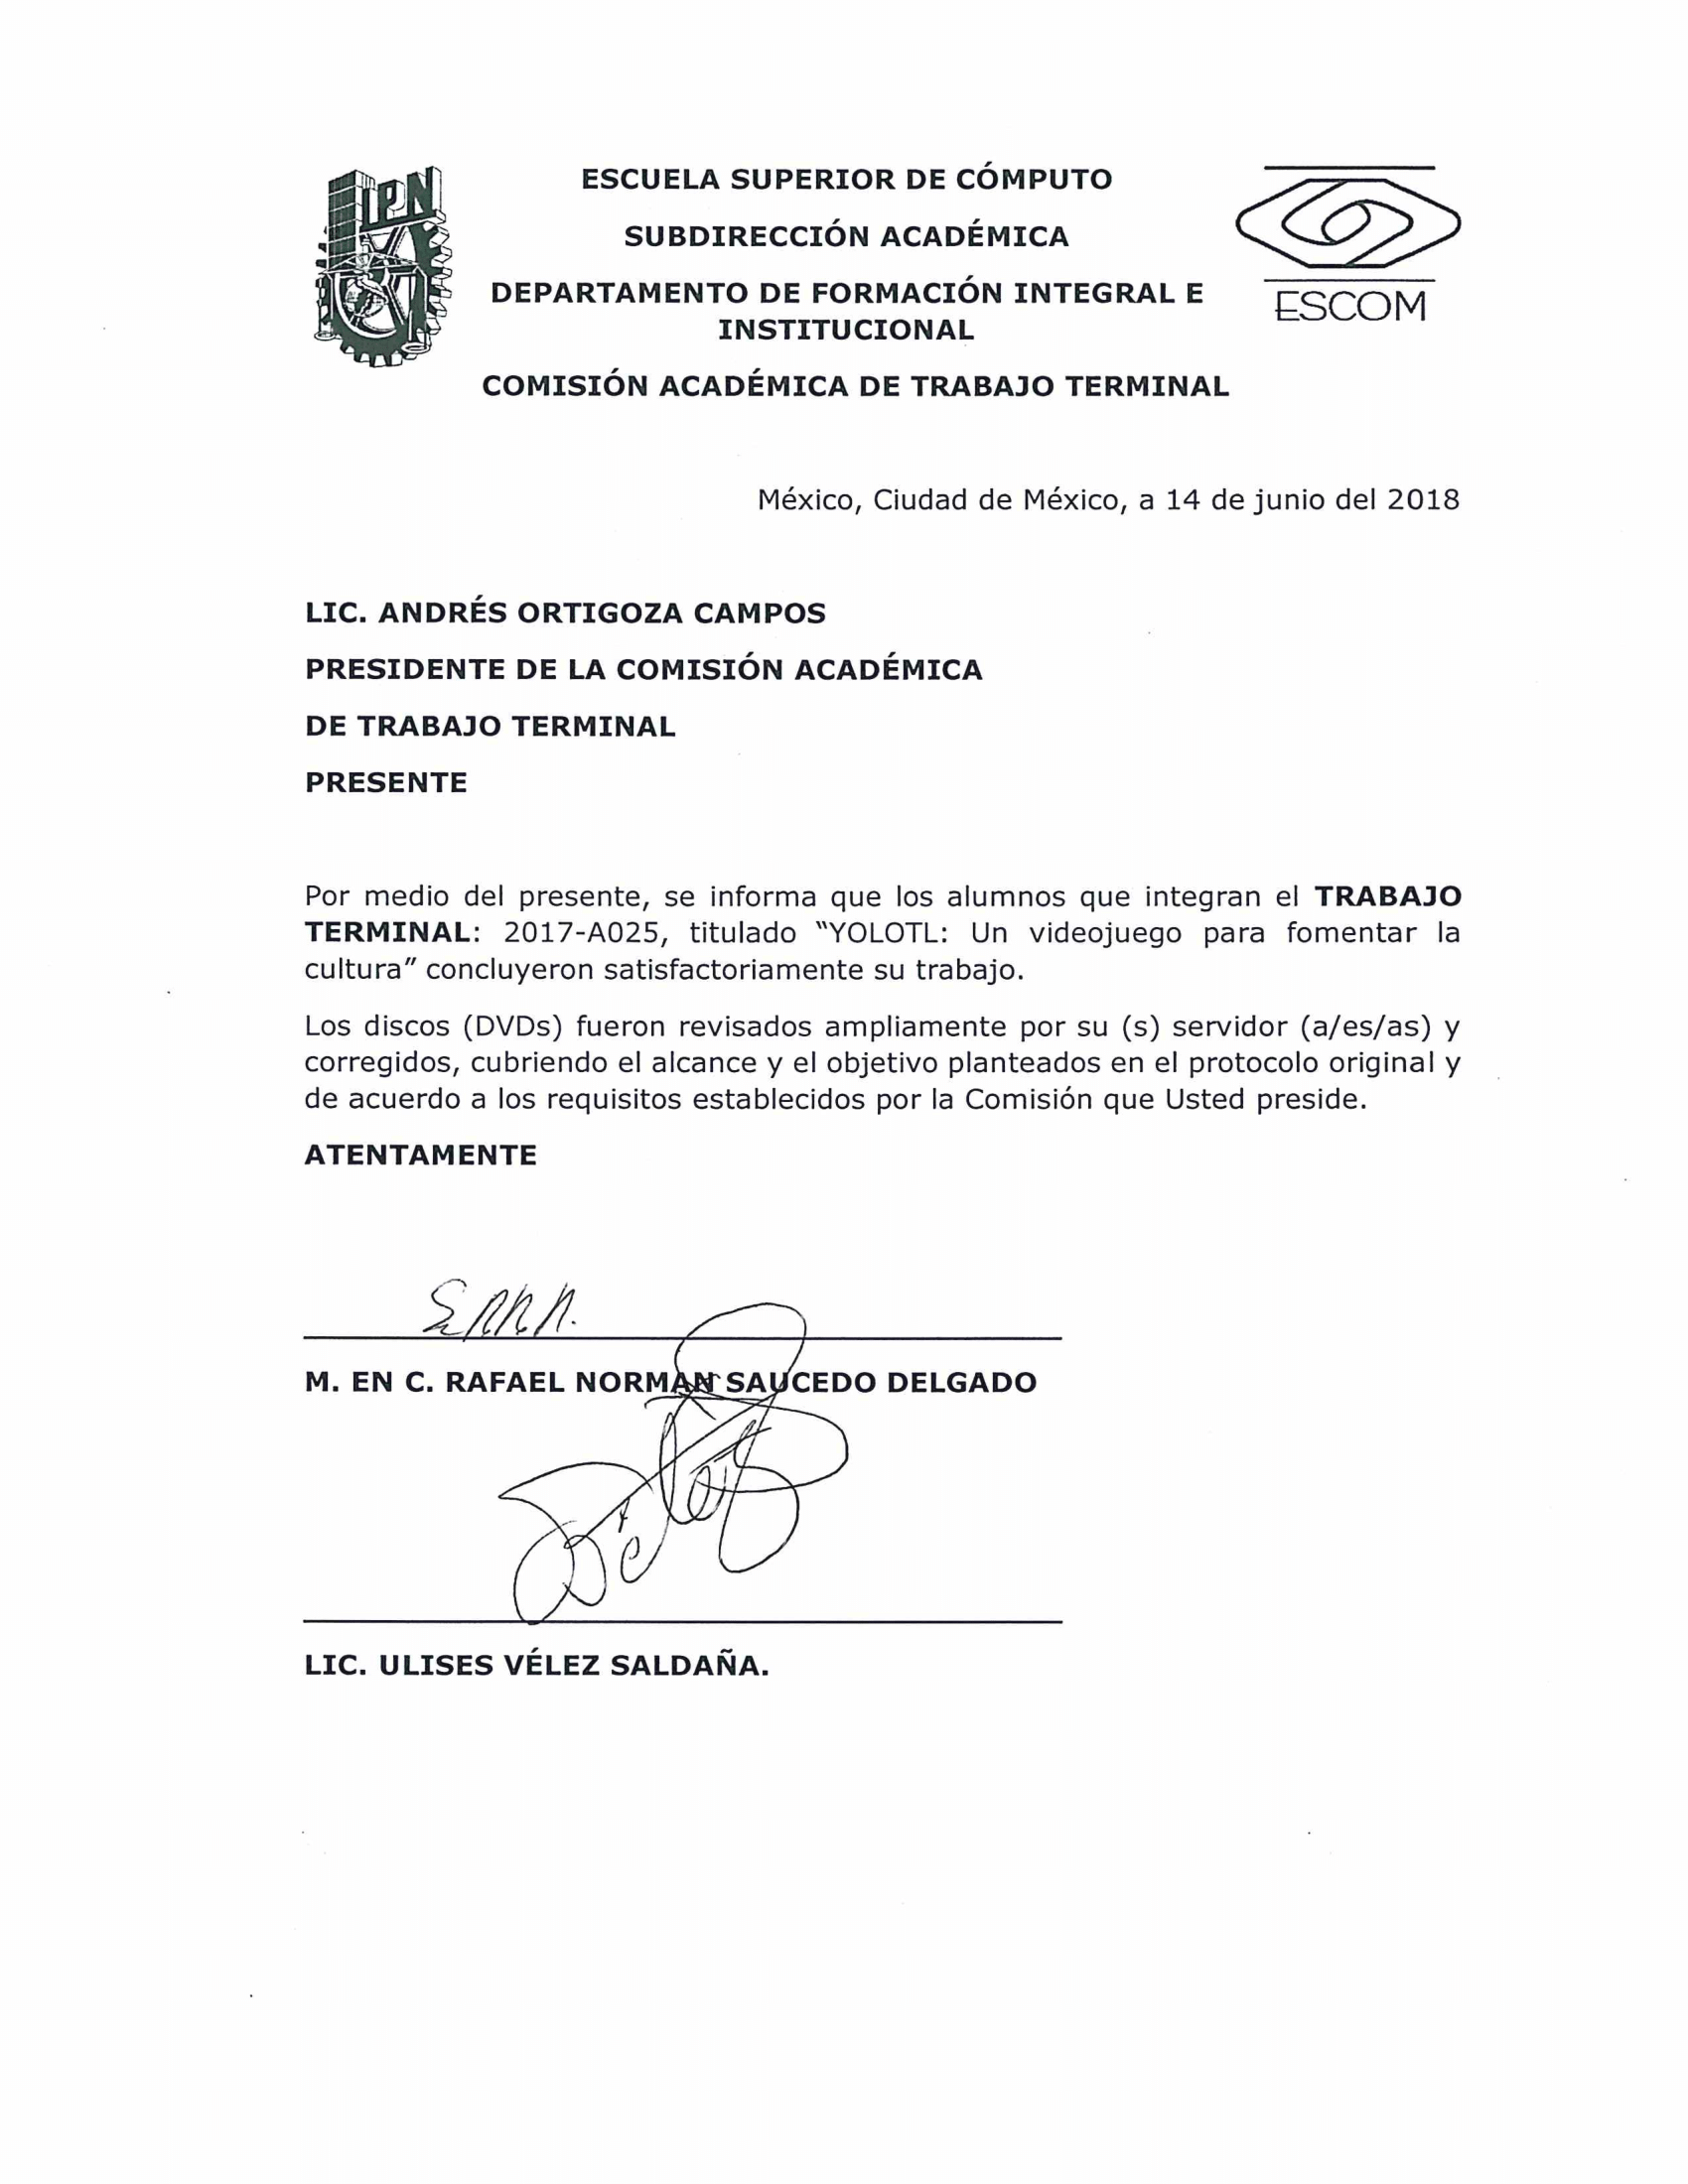
\includegraphics[width=1\textwidth]{imagen/compromiso.png}
\end{figure}

\chapter{Advertencia}

%\fcolorbox{red}{white}{
``Este documento contiene información desarrollada por la Escuela Superior de Cómputo del Instituto Politécnico Nacional, a partir de datos y documentos con derecho de propiedad y por lo tanto, su uso quedará restringido a las aplicaciones que explícitamente se convengan.”  La aplicación no convenida exime a la escuela su responsabilidad técnica y da lugar a las consecuencias legales que para tal efecto se determinen. Información adicional sobre este reporte técnico podrá obtenerse en: La Subdirección Académica de la Escuela Superior de Cómputo del Instituto Politécnico Nacional, situada en Av. Juan de Dios Bátiz s/n Teléfono: 57296000, extensión 52000.
%}

	
	\tableofcontents
	
	\mainmatter
	\chapter{Introducción}
	\chapter{Antecedentes}

\section{Propuesta}
En esta sección se presenta a manera de resumen las propuestas y los conceptos 
definidos durante el trabajo terminal 1, tales como el planteamiento del problema, 
conceptos y definiciones referentes al videojuego y su desarrollo, la definición 
y delimitación de la cultura y el planteamiento de la solución que se desarrolla 
durante el trabajo terminal.  

%====== Planteamiento del problema ======%
\subsection{Planteamiento del problema}
En México existe un fuerte desinteres y desconocimiento hacia su cultura e historia 
nacional. De acuerdo con la Tercera Encuesta Nacional de Cultura Constitucional, 
el 52.7\% de los encuestados desconoce el año en que se aprobó la constitución 
nacional y no la relaciona con la Revolución Mexicana \cite{RefConsti}. Con base 
en la encuesta realizada por Parametría, empresa dedicada a la investigación 
estratégica de la opinión y análisis de resultados, solo el 32\% de su encuestados 
supó que México se independizó de España, el 51\% desconoce el país del que se 
independizó México, mientras que el resto del porcentaje de los encuestados 
piensa que México se independizó de otro país que no es España; la misma 
encuesta realizada por Parametría señala que el 25\% de los encuestados mencionaron 
personajes historicos ajenos a la independencia de México como participes de 
ésta y el 12\% respondió no saber que personajes historicos participaron en la 
independencia\cite{RefParametria}. 
 
%======Marco Teorico ======%
\subsection{Marco Teorico}
En esta sección se presentan los conceptos básicos para comprender el trabajo 
realizado durante el desarrollo del trabajo terminal, tales como la definición 
del videojuego, sus características, su clasificación, las metodologías de 
desarrollo, las herramientas para el desarrollo y la cultura. 

\subsubsection{Videojuego}
El grupo de periodista especializado en tecnología y desarrollo de software 
Carricay define al videojuego como: "una aplicación interactiva orientada 
al entretenimiento que, a través de ciertos mandos o controles, permite simular 
experiencias en la pantalla de un televisor, una computadora u otro dispositivo 
electrónico"\cite{Ref_DefVideo}.
\\
\par
Al igual que con otros productos tecnológicos, la evolución de los videojuegos 
ha sido vertiginosa, resultando complicado mencionar características comunes 
para todos los videojuegos. Sin embargo,en el libro “\textit{Marketing} y videojuegos: 
\textit{Product pacement, in-game, adevertising y 
advergaming}” se menciona que existen seis características comunes en los 
videojuegos: Interactividad, entretenimiento, jugabilidad, simulación \textbackslash 
virtualidad, inmersión y multiplataformidad\cite{RefCarac}; a continuación se 
menciona en que consisten cinco de las seis características, esto debido a que 
la última no se encuentra presente en todos los juegos y el mismo autor de la 
obra la menciona como una caracteristica opcional a tomar en cuenta:

	\begin{itemize}
		\item \textbf{Interactividad:} En el articulo "\textit{Defining Virtual Reality:
		 Dimensions Determining Telepresence}" se define la interactividad como la 
		 capacidad de los usuarios para participar y modificar la forma y el contenido 
		 de un entorno mediado en tiempo real\cite{RefInteractividad}.  
		
		\item \textbf{Entretenimiento:} en el articulo "Las Tecnologías del
		 Entretenimiento: Pasado, Presente y Futuro", el entretenimiento "se asocia, 
		 usualmente, de hacer algo que nos divierte, algo que podemos hacer solos o con 
		 otros, para entretenernos o divertirnos, en nuestro tiempo libre, o tal vez, 
		 algo que nos relaje o que nos haga reír"\cite{RefEntretenimiento}. 
		
		\item \textbf{Jugabilidad:} en el libro “\textit{Marketing} y videojuegos: 
	\textit{Product pacement, in-game, adevertising y advergaming}” se define la 
	jugabilidad como "la relación que existe entre todas las acciones reacciones e 
	interacciones tanto del videojugador como el videojuego como entre los propios 
	sistemas y subsistemas programados en el videojuego"\cite{RefCarac}.		
	
		\item \textbf{Simulación \textbackslash Virtualidad:} La simulación "se trata 
		de una representación a medida cuyo objetivo nos permite interactuar y 
		relacionarnos con lo representado según nuestros intereses"\cite{RefCarac}.
		
		\item \textbf{Inmersión:} Con base en el libro "La vida en la pantalla: La
		 construcción de la identidad en la era de internet", la inmersión es un 
		 proceso psicológico que se produce cuando la persona deja de percibir de 
		 forma clara su medio natural al concentrar toda su atención en un objeto,
		  narración, imagen o idea que le sumerge en un medio artificial 
		  \cite{RefInmersion}. Por su parte en la tesis "Libertad dirigida: Análisis 
		  formal del videojuego como sistema, su estructura y su avataridad", la 
		  inmersión se entiende como la coherencia de la ficción del juego y su 
		  aceptación por el jugador.\cite{refInmersionNavarro}  
	\end{itemize} 

Los videojuegos pueden se clasificados con base a su jugabilidad, en el libro 
"Juego. Historia, Teoría y Práctica del Diseño Conceptual de 
Videojuegos"\cite{Ref_JuegoDisenio} se propone la siguiente clasificación.
	\begin{itemize}
		\item \textbf{Juegos de acción:} Son juegos usualmente de temática 
				violenta. El jugador lucha por su supervivencia, para ello se vale 
				de armas o habilidades de  combate. 
			%==== Juegos de estrategia ====%
				\item \textbf{Juegos de estrategia:} Para que el jugador logre sus 
				objetivos en este tipo de juegos, éste debe de planear una estrategia, 
				normalmente a lago plazo. 
			%==== Juegos de Rol ====%
				\item \textbf{Juegos de Rol:} La mecánica de los juegos de rol gira 
				en torno a un grupo de héroes, con habilidades y progresión definidos; 
				el grupo de héroes debe de trabajar coordinadamente para cumplir un 
				objetivo; estos héroes pueden ser controlados por un solo jugador o 
				por varios. El jugador deberá explorar un mundo de gran tamaño 
				haciendo evolucionar a	sus personajes y sus habilidades. 
				\item \textbf{Videojuego de aventura:} Son parecidos a los juegos de 
				Rol; con la peculiaridad de que tienen una progresión más lineal y no 
				se hace tanto énfasis en los combates, siendo su eje principal la 
				narrativa.
				\item \textbf{Videojuegos de deportes:} Son todos aquellos videojuegos 
				que tratan sobre deportes que no involucren la conducción de un 
				vehículo. Pueden ser juegos sobre fútbol, fútbol americano, tenis, etc.
				\item \textbf{Videojuegos de carreras de vehículos:} Son todos aquellos 
				se centran en las carreras con todo tipo de vehículos, mayoritariamente 
				automóviles.
				\item \textbf{Videojuegos {\it puzzle:}} Este tipo de juego involucra 
				la resolución de un problema a partir de la utilización de una serie 
				limitada de recursos, por lo que si los recursos no se utilizan de la 
				manera correcta el problema no podrá ser solucionado.  
	\end{itemize}
	
Dentro de la clasificación de los juegos de acción entren los juegos de plataforma, 
definidos por una jugabilidad donde el jugador debe de controlar a un personaje 
con el que se dezplazará saltando entre plataformas y esquivando todo tipo de 
obstáculos y enemigos\cite{Ref_JuegoDisenio}. 
Es importante que se entienda el concepto del videojuego, sus características, 
su clasificación y la jugabilidad básica de un juego de plataforma ya que el 
presente Trabajo Terminal gira entorno al desarrollo de un videojuego de plataforma.

\subsubsection{Metodología de desarrollo}
Las metodologías de desarrollo de software son un conjunto de procedimientos, 
técnicas y ayudas a la documentación para el desarrollo de productos software
\cite{Ref_metodologia}. Para el presente trabajo terminal se consideran las 
siguientes metodologías como candidatas a implementar para guiar el desarrollo:

\begin{itemize}
	\item \textbf{Metodología en cascada:} Sigue una progresión lineal por lo que 
	cualquier error que no se haya detectado con antelación afectara todas las 
	fases que le sigan provocando una redefinición en el proyecto y por ende un 
	aumento en los costos de producción del sistema \cite{Ref:CarCascada}.Esta 
	metodología se divide en las siguientes etapas:
		\begin{itemize}
			\item \textbf{Análisis de los requisitos del software.}
			\item \textbf{Diseño.}
			\item \textbf{Codificación.}
			\item \textbf{Pruebas.}
			\item \textbf{Mantenimiento.}
		\end{itemize}
	\item \textbf{Metodología en \textit{Scrum}:} \textit{Scrum} parte de la visión 
	general que se desea que el producto alcance; a partir de esta visión se inicia la 
	división del proyecto en diferentes módulos. \textit{Scrum} implementa una 
	jerarquía entre los módulos en donde los módulos de mayor jerarquía son los 
	que se desarrollaran al inicio del proyecto o durante las primeras iteraciones 
	o \textit{sprints} \cite{Ref_ScrumRef}.Cada sprint se compone de las siguientes 
	fases:
	\begin{itemize}
		\item \textbf{Concepto}.
		\item \textbf{Especulación}.
		\item \textbf{Exploración}.
		\item \textbf{Revisión}.
		\item \textbf{Cierre}\cite{Ref_ScrumGuia}. 
	\end{itemize}
	\item \textbf{Metodología de Programación extrema:} Es una metodología de 
	desarrollo ágil y adaptable, soporta cambios de requerimientos sobre la marcha. 
	Su principal objetivo es aumentar la productividad y minimizar los procesos 
	burocráticos, por lo que el software funcional tiene mayor importancia que la 
	documentación\cite{Ref_XP}.
	\item \textbf{Metodología \textit{Huddle}:} Es una metodología cuya funcionalidad 
 se basa en la metodología \textit{Scrum}, con la diferencia de que está orientada al
  desarrollo de videojuegos.  De naturaleza ágil, resulta óptimo para equipos 
  multidisciplinarios de 5 a 10 personas; es iterativa, incremental y evolutiva 
  \cite{Ref_Huddle}. \textit{Huddle} se divide en las siguientes etapas:
  	\begin{itemize}
  		\item \textbf{Preproducción}.
		\item \textbf{Producción}.
		\item \textbf{Postmorten}.
  	\end{itemize}
\end{itemize}

Tras un riguroso análisis comparativo entre metodologías, se elige a 
\textit{Huddle}  como la metodología a guiar el desarrollo del Trabajo Terminal; 
esta elección se basa principalmente en que dicha metodología esta enfocada a 
videojuegos y no requiere ser adaptada por lo que se puede llevar a cabo el 
proyecto de manera directa sin tener que invertir tiempo en adaptar la metodología 
a las necesidades del desarrollo de un videojuego.

\subsubsection{Herramientas de desarrollo}
Como cualquier desarrollo de software, el desarrollo de un videojuego requiere 
se software especializado tal como un motor de juego, editores de imágenes, software 
de diseño, de edición de audio, etc. En este apartado se van a definir algunas de 
las herramientas utilizadas durante la elaboración del trabajo terminal.
\\
\par
La primera herramienta a definir es el del motor de juego. El motor de juego, 
también conocido como \textit{Game Engine}, parte del concepto de reutilización; 
es decir, es posible generar juegos a partir de un código base y común mediante una 
separación adecuada de los componentes fundamentales, tal como visualización de 
gráficos, control de colisiones, físicas, entrada de datos etc \cite{Ref:MutorGraf}; 
esto permite a quienes trabajen en un juego puedan centrarse en todos aquellos 
detalles que hacen al juego único. Dentro del mercado existen diferentes 
opciones de motores de juego tales como \textit{Unity3D}, \textit{UnrealEngine} 
y \textit{CryEngine}, por citar algunos. Para el presente trabajo terminal se 
decide por utilizar \textit{Unity3D} ya que ofrece: 

	\begin{itemize}
		\item Desarrollo muliplataforma, lo que permite aumentar la escalabilidad 
		del proyecto. 
		\item Curva de aprendizaje rápido.
		\item Comunidad de desarrolladores activa.
		\item Tres opciones de lenguajes de programacion para utilizar: 
		\textit{$\sharp C$,javaScript y Boo}.
		\item No requiere de muchos recursos para su instalación.
		\item Uso de diferentes tipos de licencia lo que permite contar con una 
		licencia gratuita, de pago y una de negocios. No existiendo mucha diferencia 
		de funcionalidad entre la licencia libre y la de pago.
	\end{itemize}
 En lo que refiere a la creación del entorno gráfico del videojuego, es decir de 
 sus sprites, se decide utilizar los \textit{software} de diseño 
 \textit{Adobe Phtoshop} y \textit{Corel Draw}. Ya que al momento de elegir dichos 
 softwares ya se contaba con experiencia previa sobre su funcionamiento y no 
 requiere ningún tipo de periodo de prueba para familiarizarse con su funcionamiento. 
 Ambos \textit{softwares} son de pago y para el desarrollo del presente trabajo 
 terminal se utiliza una licencia personal por lo que si se desea comercializar 
 el juego va a ser necesario adquirir otro tipo de licencia para le generación 
 de \textit{sprites}.


\subsubsection{Cultura}
Una vez explicado lo que es el videojuego, su metodologia de desarrollo y las 
herramientas a usar para desarrollarlo, es preciso definir lo que es la cultura; 
para tal objetivo el presnete trabajo se vale de la definición propuesta por la 
Organización de las Naciones Unidas para la Educación, la Ciencia y la Cultura 
(UNESCO, por sus siglas en inglés). La UNESCO define la cultura como “el conjunto 
de los rasgos distintivos, espirituales y materiales, intelectuales y afectivos 
que caracterizan a una sociedad o un grupo social. La cultura engloba, además 
de las artes y las letras, los modos de vida, los derechos fundamentales al ser 
humano, los sistemas de valores, las tradiciones y las creencias; de igual forma 
la cultura da al hombre la capacidad de reflexionar sobre sí mismo\cite{RefCultura}”. 
Bajo su misma definición la UNESCO, se plantea que la importancia de la cultura 
radica en su capacidad de hacer a los seres humanos racionales, críticos y 
éticamente comprometidos; ya que, través de ella se disciernen los valores y se 
efectúan opciones. Siendo por medio de ella que el hombre se expresa, toma conciencia 
de sí mismo, se reconoce como un proyecto inacabado, pone en cuestión sus propias 
realizaciones, busca incansablemente nuevas significaciones, y crea obras que lo 
trascienden \cite{RefCultura}.
\\
\par
Para efectos del presente trabajo terminal, este únicamente va a abordar la cultura 
de carácter historica, es decir la cultura que hace referencia a la herencia social, 
es decir aquella que relaciona a la sociedad con su pasado
\cite{RefculturaClasificacionEl}.

\subsection{Planteamiento de la solución}
Con el fin de fomentar la cultura y la historia se desarrolla Yolotl, un videojuego 
de plataforma y aventuras en dos dimensiones para dispositivos móviles android 5.1 
de gama media alta.
\\
\par
Las razones por las que se aborda la solución del problema con un videojuego se 
debe principalmente a diferentes factores tales como:

\begin{itemize}
	\item \textbf{El estado de la industria mexicana de los videojuegos:} En el 
	2017 México ocupó el 12 puesto en cuanto a consumo de videjuegos percibiendo 
	un ingreso de 1.4 mil millones de dolares en esta industria. A su vez México 
	cuenta con 49.2 millones de jugadores\cite{Ref_JuegosGanancia}.

	\item \textbf{El auge de los juegos para teléfonos móviles:} En el 2017 la 
	industria del videojuego tuvo ganancias de 108.9 mil millones de dolares de 
	los cuales el 32\% de las ganancias fueron generadas por los teléfonos 
	inteligentes y un 10\% por las tablets; con este porcentaje los teléfonos 
	superaron a las consolas de mesa en ingresos\cite{Ref_JuegosGanancia}. 

	\item \textbf{El consumo de teléfonos móviles en México}: En el 2017 México 
	contaba con 52 millones de usuarios de teléfonos móviles, lo que lo ubicó en 
	el 9 puesto a nivel mundial en el consumo de teléfonos inteligentes
	\cite{Ref_TelefonosGanancia}.

	\item \textbf{La interactividad de un videojuego:} Como se menciona en el 
	artículo \textit{Identification with the Player Character as Determinant 
	of VideoGames Enjoyment}: en los videojuegos, la interactividad juega un 
	papel importante para identificar y adoptar un determinado concepto, ya que 
	dentro del videojuego el jugador no es un espectador, pues participa 
	directamente en la historia e interactúa con el mundo del personaje; esto 
	genera una relación íntima entre el jugador y el personaje puesto que es 
	gracias al jugador que el personaje puede avanzar en la historia y a su vez 
	es gracias al personaje que el jugador puede interactuar con la historia
	\cite{PlayerIdentification}. 
\end{itemize}
\section{Ajustes}
En esta sección se definen todas las nuevas estrategias a seguir para agilizar y 
optimizar el desarrollo del juego.

\subsection{Correción del enfoque de la solución}

\subsection{Nueva división de trabajo}
Antes del inicio del tercer \textit{sprint} y teniendo como base la experiencia 
de desarrollo los anteriores prototipos, queda claro que se necesita diseñar una 
nueva estrategia que permita agilizar el desarrollo del juego sin comprometer 
la calidad del mismo. Por tal motivo se decide reorganizar la asignación de 
tareas, en lugar de que los miembros del equipo de desarrollo se encarguen del 
mismo nivel, se reparten los niveles restantes del desarrollo entre los 
integrantes del equipo. Quedando la asignación de los niveles como se ve en la 
figura \ref{fig:Tareas} .

		\begin{figure}[h]
    			\centering
    			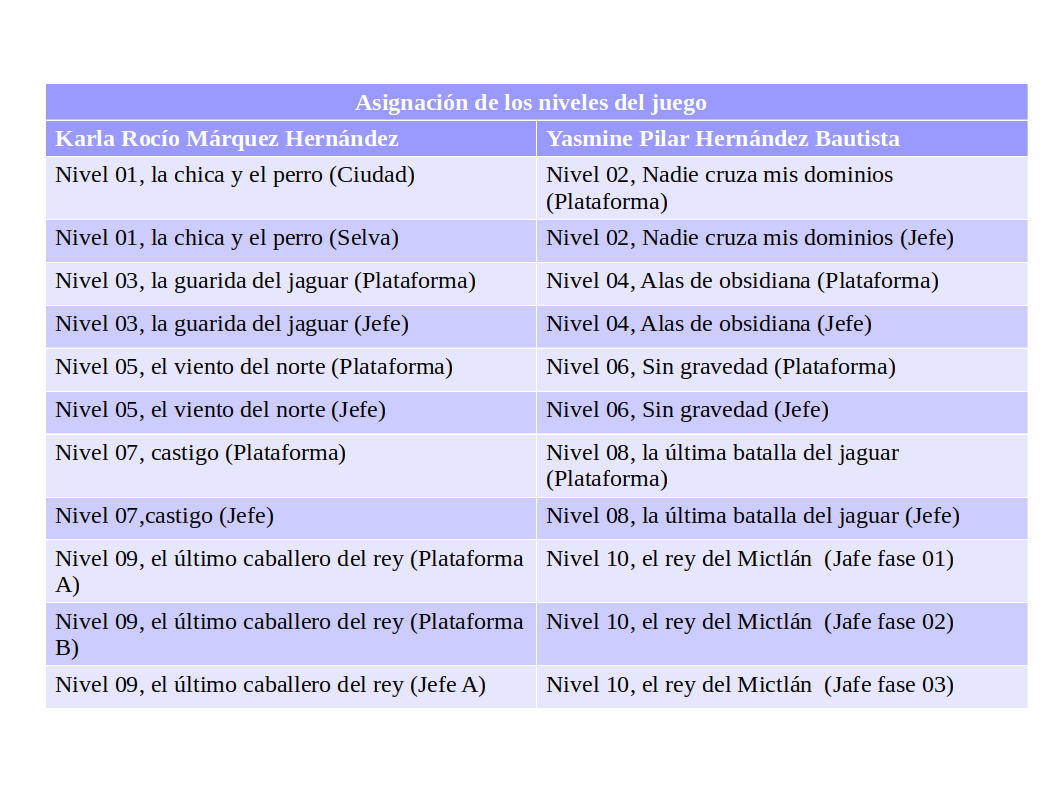
\includegraphics[width=0.8\textwidth]{02Antecedentes/Imagenes/tareasAsignacion.png}
    			\caption{Asignacion de tareas}
    			\label{fig:Tareas}
		\end{figure}


Esta división de trabajo permite que los niveles se desarrollen de manera paralela y no de manera secuencial como se había trabajado hasta este \textit{sprint}; simulando de esta forma un flujo de trabajo similar a procesamiento multihilo, en el que cada integrante del equipo es un hilo y desarrolla sus tareas de manera paralela al otro.

\subsection{Actualizando el motor de juego}
Paralelamente a la nueva asignación de tareas, fue liberada la versión 
2017.3.1f de \textit{Unity3D}. Esta versión incluye herramientas que agilizan la 
creación de niveles como el uso de: 
	\begin{itemize}
		\item \textbf{\textit{Tilemap}:} Herramienta para el mapeado de niveles. Esta 
		herramienta facilita la creación de mapas al crear una malla sobre la que 
		se arrastraran diferentes \textit{Sprites} que se hayan importado previamente 
		al tilemap (ver figura \ref{fig:TilemapPantalla}). En la sección () se 
		profundizará su funcionamiento.
		
		\begin{figure}[h]
    			\centering
    			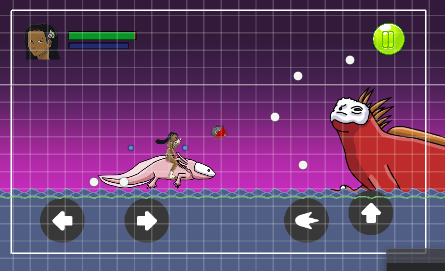
\includegraphics[width=0.6\textwidth]{02Antecedentes/Imagenes/tilemaps01.png}
    			\caption{Vista de la escena cuando se tiene un \textit{GameObject} de 
    			tipo \textit{Tilemaps} para la construcción de niveles}
    			\label{fig:TilemapPantalla}
		\end{figure}
		
		\item \textbf{\textit{Cinemachine}:} \textit{Asset} que permite controlar la 
		cámara de la escena, con este \textit{asset} se le puede indicar que objeto se 
		desea que la cámara siga y se puede asignar un área que limitara el movimiento 
		de la cámara (ver figura \ref{fig:CinemaPantalla}). \textit{Cinemachine} se 
		descarga directamente desde la tienda de \textit{assets} de \textit{Unity} y 
		fue desarrollado por los ingenieros de \textit{Unity}, lo que significa que 
		no genera conflictos o no requiere de configuraciones extras al proyecto para 
		importar. En la sección () se profundizará su funcionamiento.
			
			\begin{figure}[h]
    			\centering
    			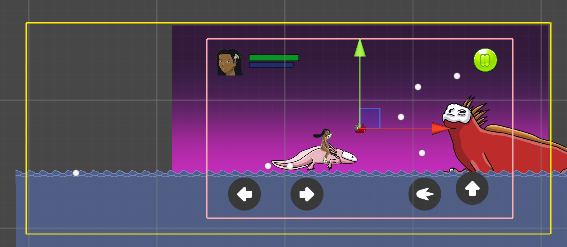
\includegraphics[width=0.6\textwidth]{02Antecedentes/Imagenes/cinemachine01.png}
    			\caption{Vista de la escena cuando se tiene un \textit{GameObject} de 
    			tipo \textit{Tilemaps} para la construcción de niveles}
    			\label{fig:CinemaPantalla}
			\end{figure}

		\item \textbf{\textit{Sprite Packer}}: Si bien no es una herramienta para 
		construcción de niveles o un \textit{asset}, esta herramienta es una de las 
		más útiles que se agregó a la nueva versión de \textit{Unity} ya que, como 
		su nombre lo indica, permite el empaquetado de \textit{sprites} (ver figura ). 
		Empaquetar 
		los \textit{sprites} es una práctica que optimiza el renderizado de objetos, 
		ya que el controlador de gráficos de \textit{Unity} realiza una sola llamada 
		por paquete cuando renderiza los objetos y con esa única llamada renderiza todos 
		los objetos de la escena que se encuentren en ese paquete; si los 
		\textit{sprites} no se encontraran dentro de un paquete el controlador de 
		gráficos de \textit{Unity} haría una llamada por cada \textit{sprite}.  
			\begin{figure}[h]
    			\centering
    			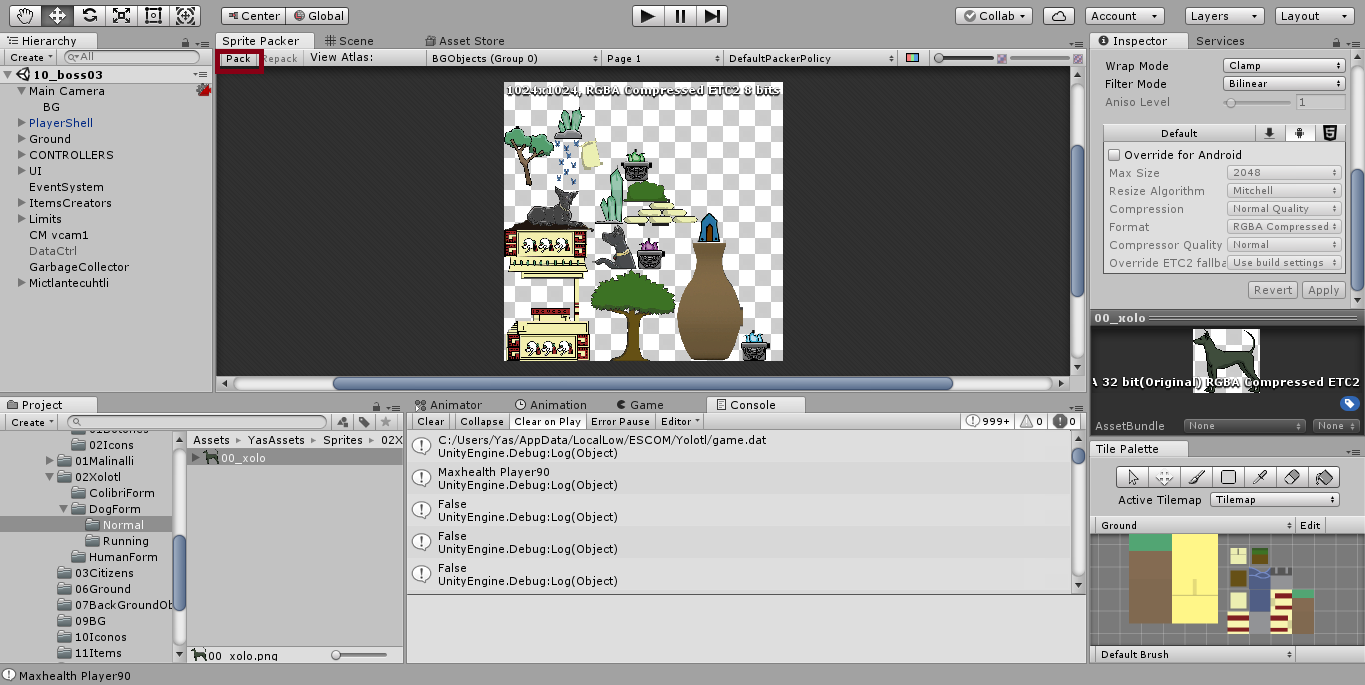
\includegraphics[width=0.6\textwidth]{02Antecedentes/Imagenes/01.png}
    			\caption{Vista de la pestaña del \textit{Sprite Packer}.}
    			\label{fig:CinemaPantalla}
			\end{figure}
	\end{itemize}
	Por el impacto que tendrían las nuevas herramientas de la versión de 
	\textit{Unity}, se propusó utilizarla en lugar de la versión 5.6.2f1. Antes 
	de actualizar la versión de \textit{Unity} se investigó si el proyecto sufriría 
	algún impacto negativo como falta de compatibilidad de componentes por la 
	diferencia de versiones. Al comprobar que existía una total compatibilidad 
	entre ambas versiones en cuanto a trasladar un proyecto de la versión 5.6.1f 
	a la versión 2017.3.1f. Se determinó que la nueva versión de \textit{Unity} 
	sería la que se emplearía para el resto del desarrollo del juego.
\section{Contribuciones}

En esta sección se presentan las soluciones a las observaciones realizadas por 
los sinodales durante la presentación del trabajo terminal 1.

\subsection{El juego}\label{juego}
El juego definida por la RAE es una actividad  recreativa o de competición sometida a reglas por el entretenimiento. Sin embargo más que ello es parte fundamental parael desarrollo y aprendizaje de cualquier individuao. Esta actividad contribuye a la maduración, potencia cognitiva, desarrollo emocional, vehículo emocional que contribuye para aprender nuevas habilidades y conceptos a través de su propia experiencia.

El juego refleja la percepción de sí mismos, de otras personas y del mundo que nos rodea. Por ello mismo cuenta con 5 grandes ventajas:
\begin{itemize}
	\item El juego otorga placer y felicidad.
	\item En el juego no se tiene miedo al error.
	\item Fomenta la creatividad.
	\item Práctica de creación de estrategias y colaboración.
	\item El juego es el aprendizaje natural de las personas.
\end{itemize}
	
\subsubsection{Teorías del aprendizaje}
Es el estudio del aprendizaje que concierne al proceso por el que ocurre según el libro "Teorías del aprendizaje" \cite{libroTeoApr}. Pues se necesita comprender algunas suposiciones generales de las teorías que sustentan el aprendizaje humano y de la forma en la que se construyen sus principios.

Las teorías más reconocidas sobre el aprendizaje son:
\begin{itemize}
	\item Gestalt: reestructuración perceptual.
	\item Piaget: Constructivismo genético.
	\item Vygotsky: Teoría sociocultural.
	\item Ausbel: Teoría del aprendizaje significativo.
	\item Bruner: Teoría cognitiva.
\end{itemize}

Aquella más cercana al juego para el trabajo a realizar es la teoría de Bruner. Pues el jugador que contempla es epistémico social, inserto en una cultura y estructurado por un lenguaje. La inteligencia esta relacionada con 3 etapas de desarrollo para conocer: ejecución, impresión o imagen y significado simbólico. La evaluación está enfocada al estudio integral de los procesos cognoscitivos y los cambios que se originan.


\subsubsection{Los videojuegos como medio de comunicación}
Los videojuegos gracias a sus características de alcance masivo y presentación interactiva al usuario, son considerados parte de las TIC (tecnologias de la información y comunicación). Estos son más atractivos e influyentes dado que se enfoca a el ocio y entretenimiento de las personas. 
Es así como podemos ver incluso a los videojuegos usados como publicidad, puede ser de manera implícita donde se muestre marcas o productos dentro de un escenario o situación del juego o explícita donde el mismo juego presenta a la marca mostrando sus cualidades y ventajas (en la mayoría de los casos de forma exagerada). Además podemos ahora combinar la expansión que nos da el internet junto con la diversión de un videojuego, posibilitando a los jugadores la capacidad de promover los productos que han probado y enseñarlo a los demás jugadores.


\subsubsection{Serious games}
Aquí podemos aprovechar la creación de un serious game, pues son los juegos digitales con una finalidad explícita para el aprendizaje más allá del entretenimiento sin ser pensados en la diversión. Tienen su interés en el desarrollo de las competencias, mediante actividades interactivas basadas en el juego.
Contribuyen al desarrollo de la coordinación ojo-mano, agudeza visual, reacción, atención múltiple, aptitud relacional, motivación, tolerancia a la frustración, toma de riesgos, resolución de problemas y toma de desiciones, así como la reflexión estratégica, la creatividad, cooperación y sentido de innovación {marqués, 2010, p.276}. Así mismo el jugador mejora el desempeño y se adentra a la experimentación, dada una situación simulada en la realidad virtual sin tener que enfrentar los riesgos de la realidad. 

La gamificación y game-based learning son herramientas que persiguen el mismo objetivo de atraer y hacer practicar experiencias para memorizar y retener contenidos. Pueden usarse como ayuda para crear un serious game.

La gamificación es el uso de elementos de juego y técnicas de diseño para potenciar la motivación y compromiso de los jugadores. Mientras game-based learning se refiere al área cognitiva y apariencia donde debe crearse una experiencia de aprendizaje positiva.

En el siguiente cuadro\cite{gabale} establecemos las diferencias más destacadas en ambás técnicas.

\begin{table}[htbp]
	\centering
	\caption{Diferencias entre gamificación y game-based learning}
	\label{gabale}
	\begin{tabular}{ll}
		Gamificación                                                        & Game-based learning                                                         \\
		Incluir los mecanismos de los juegos a situaciones de aprendizaje   & Usar los juegos para crear una experiencia de aprendizaje                   \\
		Existen como motivadores puntos de experiencia, logros e incentivos & La experiencia va dirigida al pensamiento crítico y resolución de problemas \\
		Enriquece la ambientación y simulación del aprendizaje              & Ambientación y simulación controlada a solo eventos positivos              
	\end{tabular}
\end{table}

\subsubsection{Motivos para jugar}
El área de interés para el desarrollo del trabajo es la gamificación, para ello la parte importante a conocer son los diferentes motivantes que tiene una persona al jugar.

Para determinar el perfil motivacional se tomará la "rueda de motivos"\ref{fig:rm} definida por Valderrama\cite{valde}, donde se define motivos de aproximación; aquellas personas sociales y buscan la convivencia y motivos de evitación; aquellas personas que prefieren la seguridad y estancia individual.
\begin{figure}
	\centering
	\caption{Rueda de motivos de Beatris Valderrama}
	\label{fig:rm}
	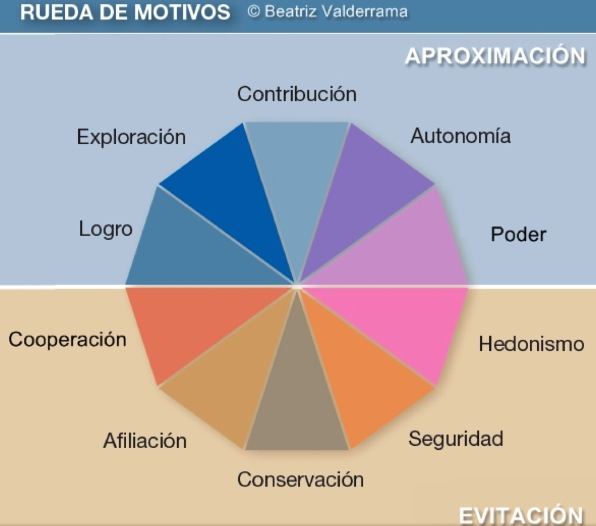
\includegraphics[width=0.5\textwidth]{imagenes\rueda-de-motivos}
\end{figure}

Es así como tenemos en contra partes diferentes motivos dependiendo del jugador obejtivo, que son la búsqueda de:
\begin{itemize}
	\item Logros o hedonismo
	\item Exploración o seguridad
	\item Contribución o conservación
	\item Autonomía o afiliación
	\item Poder o cooperación
\end{itemize}
 
\subsection{Modelo de negocios en un videojuego}\label{modeloNegocio}
Para sustentar un proyecto o producto económicamente se debe tener claro un modelo de negocios. En el mundo de los videojuegos no existe la excepción, pero también debe considerarse que existen formas muy diferentes de adquirir el ingreso.

Incluso el mismo juego puede estar involucrado en un ingreso directo del servicio.

\subsubsection{Mercado global}
Se reporta segun Newzoo \cite{newzoo2018} que 2.3 billones de jugadores en todo el mundo gastarán \$ 137.9 billones en juegos en 2018. Esto representa un aumento de + 13.3\% en comparación con el año anterior, o \$ 16.2 billones. Los ingresos por juegos digitales tomarán el 91\% del mercado global con \$ 125.3 mil millones, como podemos ver en la \ref{fig:merglo}
\begin{figure}
	\centering
	\caption{Mércado global al primer trimestre del año 2018 por Newzoo \cite{newzoo2018}}
	\label{fig:merglo}
	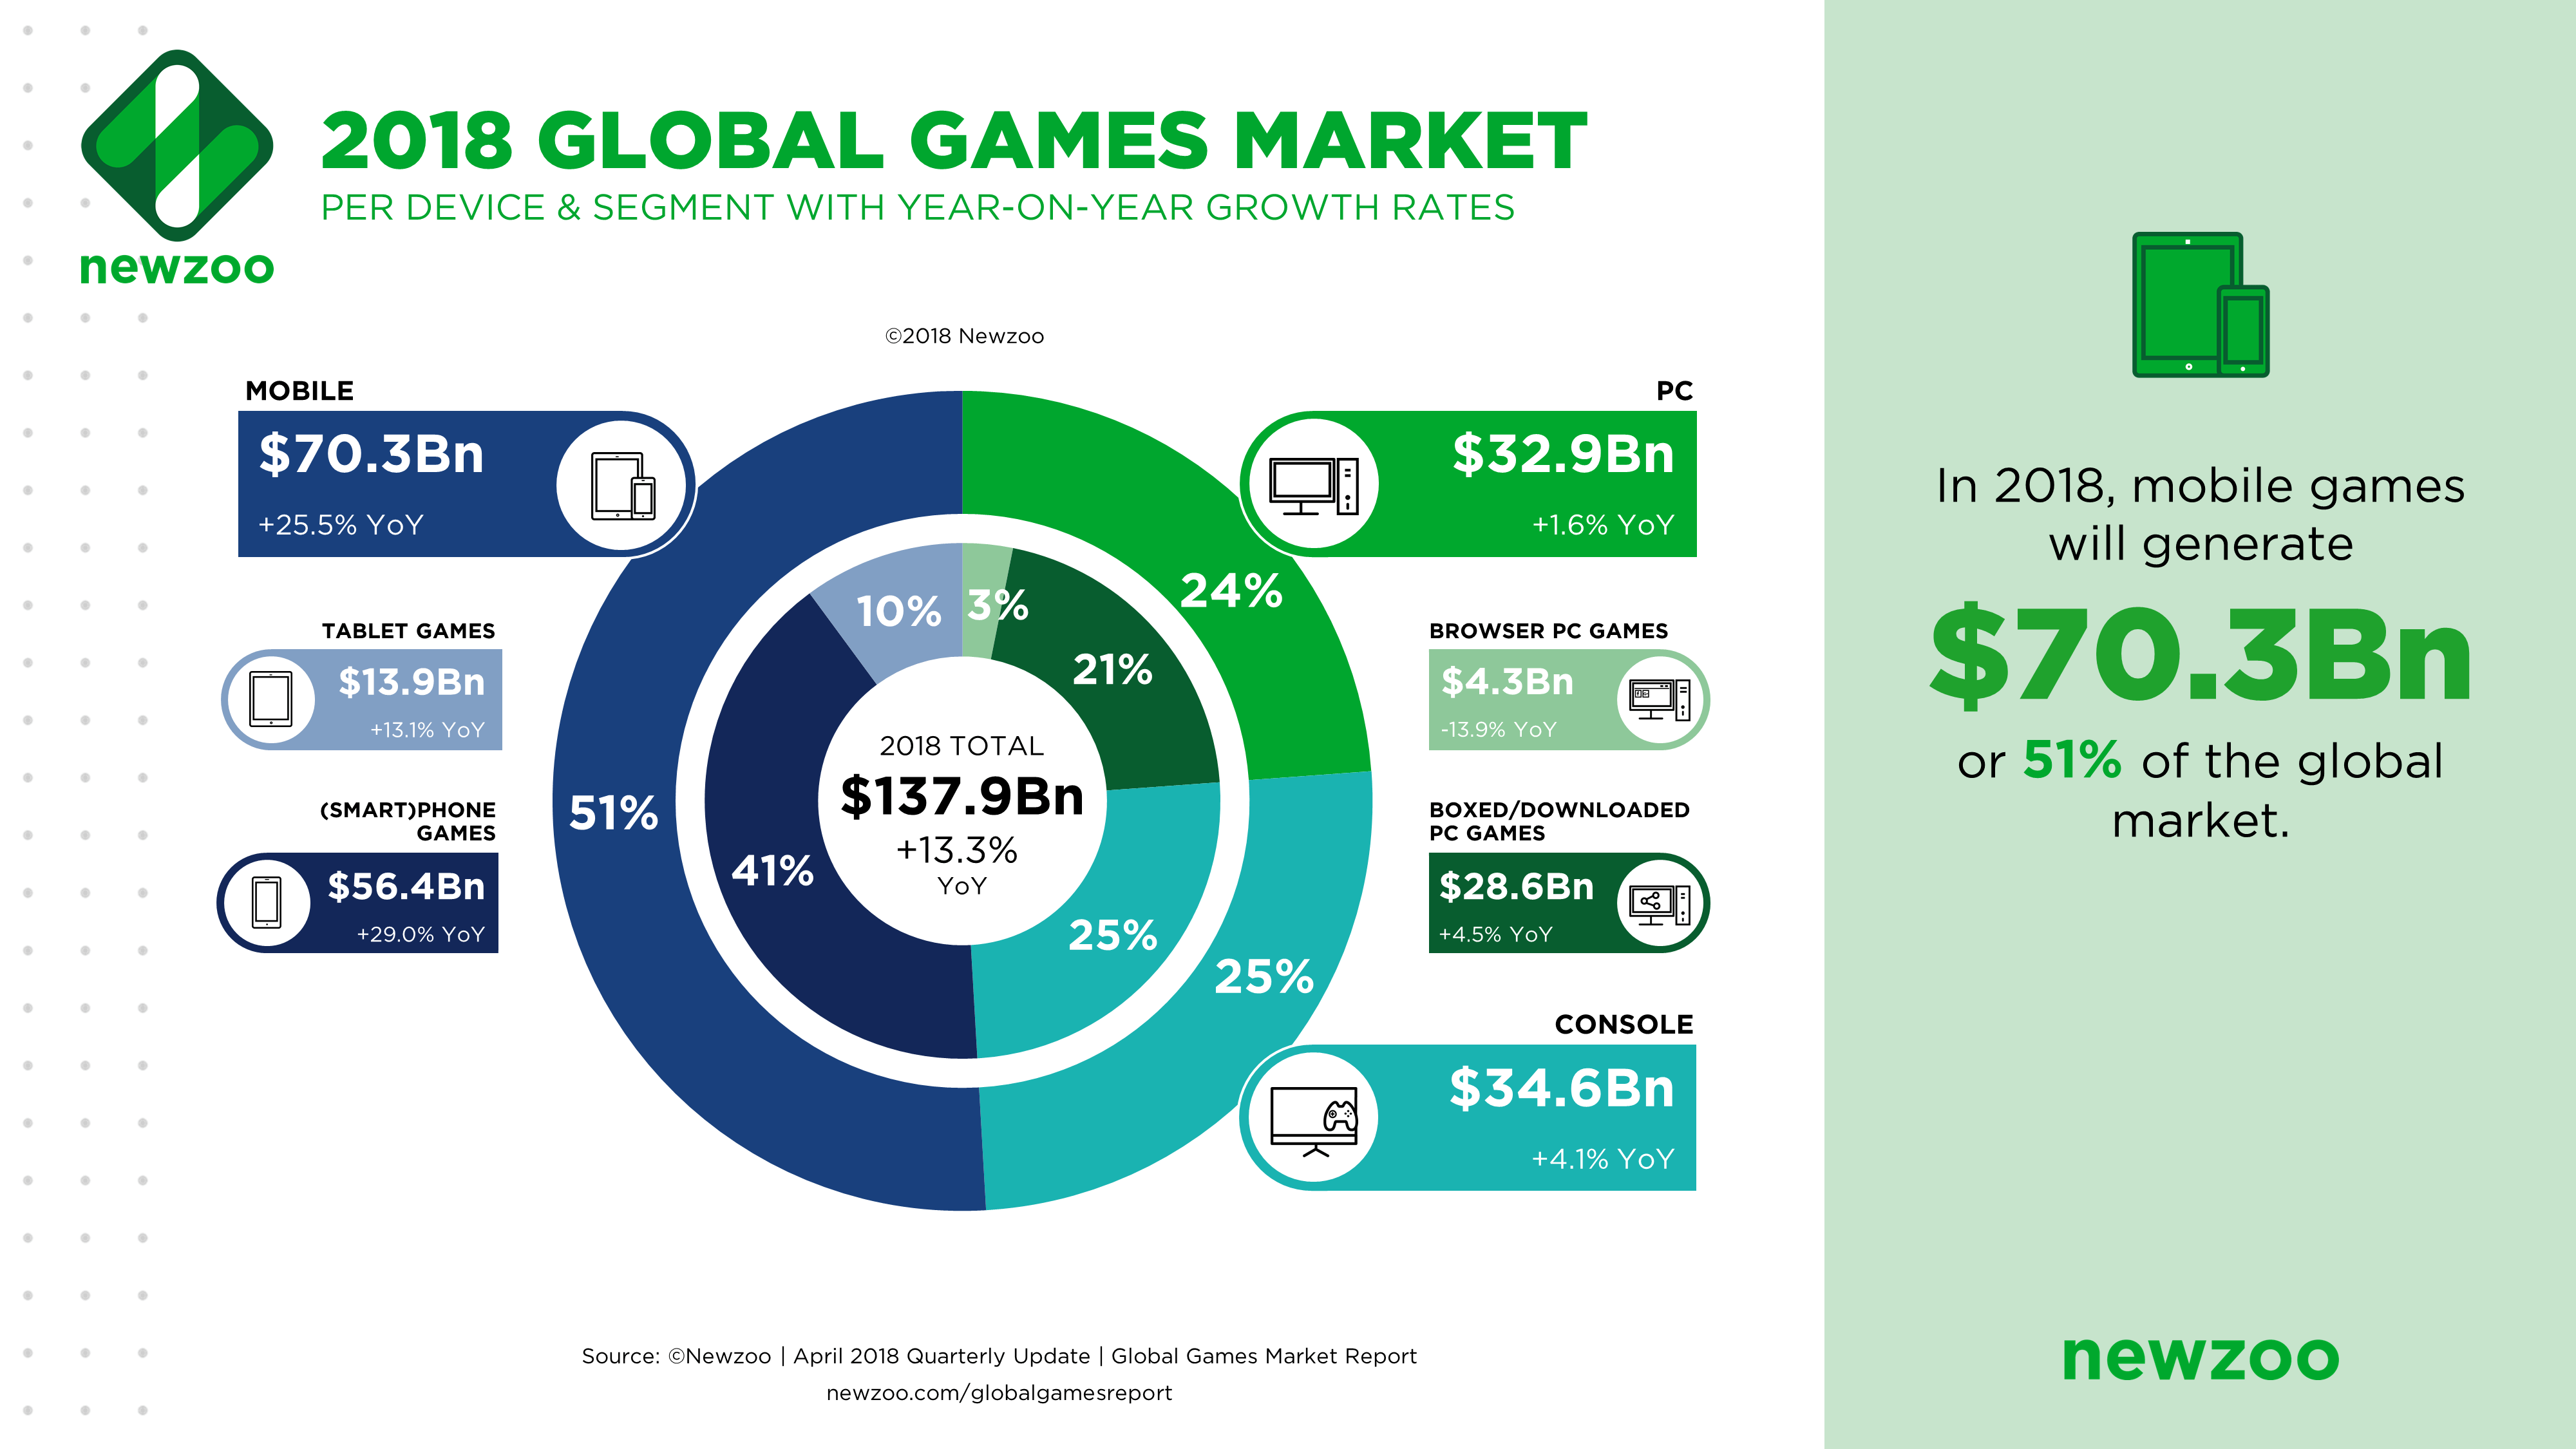
\includegraphics[width=0.5\textwidth]{02Antecedentes/contribucionesR/imagenes/merglo}
\end{figure}

Por primera vez, más de la mitad de todos los ingresos del juego provendrán del segmento móvil como vemos en la imagen{asdasd}. Los teléfonos inteligentes representarán el 80\% de esto, o \$ 56.4 mil millones, con el 20\% restante proveniente de tabletas.

\subsubsection{Salarios}
Para realizar un videojuego se necesita de diferentes profesiones para llevarlo a cabo.
En el siguiente cuadro \ref{tab:tablacostos} se mostrará la profesion y salario a recibir en la industria del videojuego en una empresa ya establecida al año 2014 segun la encuesta con una relación definida en experiencia.

% Please add the following required packages to your document preamble:
% \usepackage{multirow}
\begin{table}[htbp]
	\centering
\caption{Tabla de salarios dados en una empresa formal de videojuegos}
\label{tab:tablacostos}
\resizebox*{\linewidth}{!}{
	\begin{tabular}{|l|l|l|l|l|}
		\hline
		\textbf{Rama}                                                        & \textbf{Profesión}          & \textbf{Salario con -3años de exp.} & \textbf{Salario con 3-6años de exp.} & \textbf{Salario con +6años de exp.} \\ \hline
		\multirow{3}{*}{\textbf{Programadores e ingenieros}}                 & Programador                 & \$71,855 USD                        & \$79,877 USD                         & \$103,789 USD                       \\ \cline{2-5} 
		& Programador principal       &                                     & \$94,877 USD                         & \$116,151 USD                       \\ \cline{2-5} 
		& Director técnico            &                                     &                                      & \$135,781 USD                       \\ \hline
		\multirow{3}{*}{\textbf{Artistas y animadores}}                      & Animador                    & \$50,000 USD                        & \$55,547USD                          & \$82,230 USD                        \\ \cline{2-5} 
		& Artista principal           &                                     & \$71,029 USD                         & \$71,87576 USD                      \\ \cline{2-5} 
		& Director de arte            &                                     &                                      & \$110,000 USD                       \\ \hline
		\multicolumn{1}{|c|}{\multirow{2}{*}{\textbf{Diseñadores de juego}}} & Diseñador de juego          & \$53,000 USD                        & \$65,516 USD                         & \$77,768 USD                        \\ \cline{2-5} 
		\multicolumn{1}{|c|}{}                                               & Director creativo           &                                     & \$68,654 USD                         & \$101,944 USD                       \\ \hline
		\multicolumn{1}{|c|}{\multirow{3}{*}{\textbf{Productores}}}          & Productor asociado          &                                     & \$59,079 USD                         & \$61,912 USD                        \\ \cline{2-5} 
		\multicolumn{1}{|c|}{}                                               & Lider de proyecto           &                                     & \$73,500 USD                         & \$93,160 USD                        \\ \cline{2-5} 
		\multicolumn{1}{|c|}{}                                               & Productor ejecutivo         &                                     &                                      & \$126,833 USD                       \\ \hline
		\textbf{Profesional de audio}                                        & Director de sonido          &                                     &                                      & \$109,500 USD                       \\ \hline
		\multicolumn{1}{|c|}{\multirow{2}{*}{\textbf{Testers}}}              & Tester                      &                                     & \$38,833 USD                         &                                     \\ \cline{2-5} 
		\multicolumn{1}{|c|}{}                                               & Lider de control de calidad &                                     & \$60,417 USD                         & \$65,500 USD                        \\ \hline
		\multirow{3}{*}{\textbf{Negocios y administración}}                  & Marketing                   &                                     & \$73,500 USD                         &                                     \\ \cline{2-5} 
		& CEO                         &                                     &                                      & \$135,735 USD                       \\ \cline{2-5} 
		& Gerente ejecutivo           &                                     &                                      & \$156,731 USD                       \\ \hline
	\end{tabular}
}
\end{table}

\subsubsection{Presentación al cliente}
Un videojuego como cualquier software al momento de ser vendido al cliente puede encontrarse en dos presentaciones, una versión física o solo digital. En la siguiente tabla \ref{fiDi} se muestran las diferencias más destacables dadas por experiencia empresarial en el desarrollo por Velneo \cite{velneo2015}.

\begin{table}[htbp]
	\centering
	\caption{Tabla comparativa de un producto físico o digital por Velneo \cite{velneo2015}}
	\label{fiDi}
	\resizebox*{\linewidth}{!}{
\begin{tabular}{|l|l|l|}
	\hline
	\textbf{}                                             & \multicolumn{1}{c|}{\textbf{Físico}} & \multicolumn{1}{c|}{\textbf{Digital}} \\ \hline
	Coste de desarrollo                                   & sí                                   & sí                                    \\ \hline
	Coste de producción                                   & sí                                   & no                                    \\ \hline
	Coste de envío                                        & sí                                   & no                                    \\ \hline
	Riesgo de sobra/infra producir inventario             & sí                                   & no                                    \\ \hline
	Facturación por unidad vendida                        & mucho mayor                          & mucho menor                           \\ \hline
	Unidad vendida costea soporte                         & generalmente sí                      & imposible                             \\ \hline
	Porcentaje del precio de venta que percibe la empresa & 30\%-40\%                            & 70\%                                  \\ \hline
	Tiempo de cobro                                       & 90 días o más                        & 30 días                               \\ \hline
	Capacidad de llegar al público con marketing          & caro                                 & difícil                               \\ \hline
\end{tabular}
}
\end{table}

Aún así cabe mencionar que este es un aspecto general que involucra a cualquier software.

\subsubsection{Formas de ingreso}
Dentro de los videojuegos existen modelos de negocio que han dio cambiando a lo largo de los años y muchas de las veces depende del tipo del juego. Pero podemos definir las siguientes conforme lo visto y consumido en los últimos 5 años a la fecha del proyecto a presentar y con el apoyo de un artículo de la fundación UADE \cite{fundacionuade2014} en la tabla \ref{tablaMoneVJ}.

\begin{table}[htbp]
	\centering
	\caption{Tabla comparativa de ventajas y desventajas de modelos de negocios de videojuegos de autoría propia}
	\label{tablaMoneVJ}
	\resizebox*{\linewidth}{!}{
	\begin{tabular}{llll}
		Nombre       & Descripción                                                                                                               & Ventaja                                                                                                                                                                                                                                                                                                                  & Desventaja                                                                                                                                                                                                                                                                                                                                                                            \\
		Pay-to-play  & Se debe pagar contenido y uso del videojuego                                                                              & \begin{tabular}[c]{@{}l@{}}* Rápido retorno de inversión\\ \\ * Sin limitación de juego\\ \\ * Puede re-dirigirse a otro modelo en caso de fracaso \\ \\ * Puede ser un producto físico, por lo que puede cobrarse contenido extra\\ \\ * Complementa con compras in-game\end{tabular}                                   & \begin{tabular}[c]{@{}l@{}}* No compras por desconocimiento del juego (más en móviles)\\ \\ * Inversión grande por enfoque a consolas \\ \\ * Jugadores esperan contenido de entretenimiento de larga duración y calidad\\ \\ * No hay soporte o cambios en el juego\\ \\ * Si es un producto físico debe costearse la producción\\ \\ * Necesita publicidad\end{tabular}             \\
		Free-to-play & Ofrece gratis contenido y uso del videojuego en su totalidad, se monetiza con publicidad y compras in-game                & \begin{tabular}[c]{@{}l@{}}* Contacto con los jugadores más rápido\\ \\ * Preferente para móviles\\ \\ * Preferente para juegos de poca inversión (que quiera escalar)\\ \\ * Complementa con compras in-game\end{tabular}                                                                                               & \begin{tabular}[c]{@{}l@{}}* Depende de la cantidad de jugadores activos\\ \\ * Debe ser un juego con adicción para sustentarse\\ \\ * Debe ser un juego “infinito”\\ \\ * Requiere continuas actualizaciones si desea mantenerse\\ \\ * Debe darse al jugador contenido nuevo a jugar\end{tabular}                                                                                   \\
		Freemium     & Ofrece gratis el uso del videojuego pero no se accede a todo su contenido, establece jerarquización de tipos de jugadores & \begin{tabular}[c]{@{}l@{}}* Conveniente para demos (versión lite)\\ \\ * Oportunidad de dar a conocer el juego\\ \\ * Oportunidad de convencimiento al jugador\\ \\ * Contacto con los jugadores más rápido\\ \\ * Preferente para móviles\\ \\ * Viable aun sí existen pocos jugadores dispuestos a pagar\end{tabular} & \begin{tabular}[c]{@{}l@{}}* Debe crearse contenido de calidad por pago\\ \\ * Debe existir un control y registro de jugadores para su jerarquización\\ \\ * Usualmente el contenido extra debe ser descargado de internet (por lo que implicaría otros gastos y recursos)\\ \\ * Recomendable ser un juego “infinito”\\ \\ * A veces requiere continuas actualizaciones\end{tabular} \\
		Suscripción  & Se debe pagar el contenido y uso del videojuego pero con limitaciones.                                                    & \begin{tabular}[c]{@{}l@{}}* Es combinable con otros modelos como el freemium\\ \\ * Permite a los jugadores explorar el juego completo por cierto tiempo\\ \\ * Oportunidad de dar a conocer el juego\end{tabular}                                                                                                      & \begin{tabular}[c]{@{}l@{}}* Debe crearse contenido de calidad por pago\\ \\ * Recomendable ser un juego “infinito”\\ \\ * A veces requiere continuas actualizaciones\\ \\ * Debe darse al jugador contenido nuevo a jugar\\ \\ * Depende de la cantidad de jugadores activos\\ \\ * Debe ser un juego con adicción para sustentarse\end{tabular}         
	                           
	\end{tabular}
}
\end{table}



\subsubsection{Ingredientes de monetización}
Los modelos de negocio anteriores pueden ser combinables con otros "ingredientes" de monetización para acrecentarlos ingresos. 
\begin{itemize}
	\item Dinero virtual: Es el medio de intercambio que utiliza un videojuego para poder formalizar las compras dentro de él. A menudo se suele diferenciar el virtual currency (dinero virtual que se consigue por las propias mecánicas del juego y con abundancia) y el hard currency (dinero virtual premium que se consigue con dinero real o con acciones muy concretas y con mucha escasez).
	\item Bienes virtuales: Son objetos intangibles que son comprados e intercambiados que sólo tienen sentido dentro del juego, muchas veces estos son comprados con dinero virtual. 
	\item Publicidad y patrocinio: Anuncios o productos presentados en el juego para darse a conocer.
	\item Bonificaciones y servicios virtuales: Son aceleradores de juego o servicios que mejoran el desempeño o facilitan en el juego.
	\item DLC (downloadable content): Es un contenido de descarga digital exclusivo y adicional de un videojuego que se vende por separado y posterior al lanzamiento de este. Suele lanzarse para alargar la longevidad del videojuego y para aprovechar su éxito comercial. Su adquisición no tiene sentido sin tener antes el videojuego ya que es un producto complementario y dependiente a él.
\end{itemize}

%\subsection{Costo de hacer un videojuego}\label{costoVJ}

	
\subsubsection{Salarios}
Pararealizar un videojuego se necesita de diferentes profesiones parallevarlo a cabo.
En el siguiente cuadro se mostrará la profesion y salario a recibir en la industria del videojuego en una empresa ya establecida al año 2014 segun la encuesta ____ con una relación definida en experiencia.


\begin{table}[]
	\centering
	\caption{My caption}
	\label{my-label}
	\begin{tabular}{lllll}
		Rama                                                      & Profesión                   & Salario con \textless 3años de exp. & Salario con 3-6años de exp. & Salario con \textgreater 6años de exp. \\
		\multirow{3}{*}{Programadores e ingenieros}               & Programador                 & \$71,855 USD                        & \$79,877 USD                & \$103,789 USD                          \\
		& Programador principal       &                                     & \$94,877 USD                & \$116,151 USD                          \\
		& Director técnico            &                                     &                             & \$135,781 USD                          \\
		\multirow{3}{*}{Artistas y animadores}                    & Animador                    & \$50,000 USD                        & \$55,547USD                 & \$82,230 USD                           \\
		& Artista principal           &                                     & \$71,029 USD                & \$71,87576 USD                         \\
		& Director de arte            &                                     &                             & \$110,000 USD                          \\
		\multicolumn{1}{c}{\multirow{2}{*}{Diseñadores de juego}} & Diseñador de juego          & \$53,000 USD                        & \$65,516 USD                & \$77,768 USD                           \\
		\multicolumn{1}{c}{}                                      & Director creativo           &                                     & \$68,654 USD                & \$101,944 USD                          \\
		\multicolumn{1}{c}{\multirow{3}{*}{Productores}}          & Productor asociado          &                                     & \$59,079 USD                & \$61,912 USD                           \\
		\multicolumn{1}{c}{}                                      & Lider de proyecto           &                                     & \$73,500 USD                & \$93,160 USD                           \\
		\multicolumn{1}{c}{}                                      & Productor ejecutivo         &                                     &                             & \$126,833 USD                          \\
		Profesional de audio                                      & Director de sonido          &                                     &                             & \$109,500 USD                          \\
		\multicolumn{1}{c}{\multirow{2}{*}{Testers}}              & Tester                      &                                     & \$38,833 USD                &                                        \\
		\multicolumn{1}{c}{}                                      & Lider de control de calidad &                                     & \$60,417 USD                & \$65,500 USD                           \\
		\multirow{3}{*}{Negocios y administración}                & Marketing                   &                                     & \$73,500 USD                &                                        \\
		& CEO                         &                                     &                             & \$135,735 USD                          \\
		& Gerente ejecutivo           &                                     &                             & \$156,731 USD                         
	\end{tabular}
\end{table}

\subsection{Vicio en el videojuego}\label{vicioVJ}
Un videojuego se está convirtiendo en una adicción cuando la ansiedad se sobrepone al placer del juego y como síntoma se tiene la urgencia de jugar sin pensar en las consecuencias. El vicio se establece con cierta facilidad, ya que el juego ofrece un entorno de inmersión al combinar los aspectos interactivos e identificarse con el personaje o situación.

En la siguiente tabla se muestra las opiniones más comunes a favor y en contra de los videojuegos sin incluir mitos o falsedades, todas estás afirmaciones son demostrables o no han sido posible desmentirlas con hechos o pruebas concretas.
\begin{table}[htbp]
	\centering
	\caption{Opiniones comunes a favor y en contra de los videojuegos}
	\label{tab:tablaOpinión}
	\begin{tabular}{ll}
		A favor                                                            & En contra                          \\
		Entretienen                                                        & Provocan adicción                  \\
		Ejercitan la coordinación óculo-manual                             & Promueven conductas violentas      \\
		Estimulan la capacidad de lógica y reflexión                       & Aíslan socialmente                 \\
		Ayudan a concentrar la atención                                    & Limitan la imaginación             \\
		Son un potencial muy adecuado para distintas aplicaciones sociales & Restan tiempo de otras actividades
	\end{tabular}
\end{table}
\\[1pt]
	
\subsubsection{Síntomas de vicio}
A continuación se muestran síntomas identificables visualmente que ya representan una adicción al juego:
\begin{itemize}
	\item El jugador parece estar absorto al juego, sin atender cuando lo llaman.
	\item Siente demasiada tensión, incluso aprieta las mandíbulas cuando juega.
	\item No aparta la vista de la pantalla.
	\item Empieza a perder interés por otras actividades que practicaba.
	\item Trastornos del sueño.
	\item Distanciamiento de familia y amigos.
	\item No respeta los horarios estipulados.
\end{itemize}


\subsubsection{Carcaterísticas de un videojuego con potencial al vicio}
Los videojuegos (en especial los free-to-play) contienen características de vicio como: la necesidad de concluir “tareas incompletas”, síntomas de abstinencia y la posibilidad de jugarlo en todo momento. En este apartado solo mencionaremos algunas de ellas y almenos las más visibles en muchos videojuegos.

 \begin{itemize}
 	\item El efecto Zeigarnik: Se tiene incomodidad de las personas por tener “tareas incompletas”, en el caso de un videojuego se genera la necesidad por terminar el juego. El juego a su vez puede contemplar el nivel de porcentaje completado de un juego, provocando al jugador dicho síntoma haciéndolo jugar hasta su completado.
 	
 	\item Síntoma de abstinencia: En donde se priva o dificulta la posibilidad de realizar una actividad a una persona. En un juego tenemos como se establece turnos de juego, para recuperarlos se establece un límite de tiempo de espera. Usualmente estos tiempos de espera son de aproximadamente media hora o múltiplos de ella, pues psicológicamente este tiempo es lo que soporta una persona con una “tarea incompleta” en mente.
 	
 	\item La competencia: Que consiste en una disputa entre personas que aspiran a un mismo objetivo o a la superioridad en algo. Así, en un juego, ayudado en la mayoría de las veces por las redes sociales se puede compartir y comparar el avance entre los jugadores.
 	 \\[1pt]
 	
 \end{itemize}

\subsubsection{Causas del vicio ajenas al videojuego }
Entre los jóvenes entre 13 y 18 años especialmente existen muchas más causas para caer en el vicio de un videojuego, pueden ser factores psicológicos, emocionales, del entorno en el que se desarrollan y más. Incluso muchos de los factores siguientes encajan en otros tipos de adicciones.
\begin{itemize}
	\item Atención inexistente de los padres.
	\item No hay límites establecidos por la familia.
	\item Los valores no están asentados.
	\item Utilización de los videojuegos como "niñera".
	\item El joven no tiene sentido de pertenencia o no es aceptado en los grupos sociales que interactúa.
	\item Necesidad de escape de la realidad a un medio virtual.
	\item Establece mayor libertad expresión (o intenciones verdaderas) dentro del juego, ya sean positivas o negativas.
	\item Que la persona padezca alguna enfermedad que imposibilite realizar otras actividades .
	\item Trastornos psicológicos como depresión, impulsividad o ansiedad.
	\item Situación ante la solución de problemas y toma de decisiones.
	\item Falta de control emocional.
\end{itemize}

\subsubsection{Prevención del vicio}
Como toda adicción existen formas de prevenir llegar a ella.
Dadas las situaciones, causas, factores dentro del vicio del videojuego y con lectura de técnicas pedagógicas, las propuestas de solución se dan como sigue:

\begin{itemize}
	\item Establecer un horario de juego:
	\begin{itemize}
		\item Se puede poner una alarma que avise al jugador que ha estado jugando demasiado tiempo.
		\item Se puede programar a cierto tiempo jugado un bloqueo.
	\end{itemize}
	\item Complementariamente a la programación de un horario de juego, deberán establecerse qué actividades se llevarán a cabo en los momentos en los que no se va a jugar:
	\begin{itemize}
		\item Poder agregar al juego notas recordatorias de las actividades por hacer.
		\item Alarmas personalizadas dentro del juego.
	\end{itemize}
	\item Evitar los juegos online, al menos hasta que se tenga una organización del tiempo libre que impida dedicar mucho tiempo a dichos videojuegos.
	\begin{itemize}
		\item Evitar ser un juego online.
	\end{itemize}
	\item  No instalar la consola ni el ordenador en la habitación.
	\begin{itemize}
		\item El juego va a ser inaccesible a horas determinadas como la madrugada y noche.
	\end{itemize}
	\item Los padres deben conocer los videojuegos.
	\begin{itemize}
		\item Pedir forzosamente los correos de los tutores.
		\item Mandar mensajes a los tutores con un registro en resumen de lo que se está jugando.
		\item Habilitar una opción de bloqueo para los padres.
		\item Bloqueo automático e informe con estadística dependiendo de frecuencia de uso y tiempo de uso.
	\end{itemize}
\end{itemize}

\subsection{Modelo de datos}
La primera observación en atender fue el modelo de datos del juego, dicho modelo 
de datos se realizó utilizando un modelo entidad relación de base de datos (Ver 
Anexo \ref{Anexo:ModeloDatos}) ya que al modelarse de esta forma hace escalable 
el juego si se deseará en algún futuro emplear una base de datos para mejorar 
el almacenamiento de datos y el manejo de más usuarios para ofrecer un modo 
online. El modelo de datos está basado en el modelo de clases y contiene 
únicamente a las clases actoras. Toda entidad actora se define como una 
especialización de una entidad base llamada GameObject, esta entidad está 
definida por como su identificador y por otras entidades como GameObjectPosition, 
Level, Tag, AnimationMachine, entre otros. 

\subsection{Estrategias para combatir la adicción entre los usuarios}
La segunda observación sobre la que se trabajo fue como disminuir la adicción 
del jugador al videojuego Yolotl. Esta observación dio lugar a una investigación 
sobre la adicción a los videojuegos ya que antes de proponer alguna solución se 
debía conocer cómo se definía, las causas y las consecuencias de la adicción al 
videojuego. Al final de la investigación se pudieron formular tres posibles 
soluciones para evitar la adicción del jugador; sin embargo, dado que este tópico 
no estaba en la planeación original del proyecto y por las implicaciones que 
conllevaban cada una de las soluciones se decidió únicamente describir las 
soluciones y sus implicaciones sin desarrollar ninguna de las tres. A continuación, 
se describen a manera de resumen las soluciones (nuevamente si se dese a 
profundizar en la investigación realizada y las soluciones se puede consultar 
el Anexo \ref{Anexo:AdiccJuga}):
	\begin{itemize}
		\item \textbf{Notificación de confirmación para continuar la partida.} Esta 
		solución propone que el juego solicite la confirmación del usuario para 
		continuar una vez que éste ha detectado que el jugador ha estado jugando 
		durante un tiempo prolongado como una hora.
		\item \textbf{Control paterno.} El juego le envía un formulario al tutor del 
		jugador por medio de un correo electrónico. En este formulario el tutor podrá 
		decidir cuanto tiempo al día la aplicación podrá estar abierta. 
		\item \textbf{Sistema de vidas.} El jugador tiene una cantidad de vidas 
		limitadas. Cada vez que el jugador ingresa a un nivel o muere dentro de 
		uno y reinicia la partida se gasta una vida. Para recuperar vidas el 
		jugador deberá de esperar un determinado tiempo.
	\end{itemize}
	
%\subsection{El juego}\label{juego}
El juego definida por la RAE es una actividad  recreativa o de competición sometida a reglas por el entretenimiento. Sin embargo más que ello es parte fundamental parael desarrollo y aprendizaje de cualquier individuao. Esta actividad contribuye a la maduración, potencia cognitiva, desarrollo emocional, vehículo emocional que contribuye para aprender nuevas habilidades y conceptos a través de su propia experiencia.

El juego refleja la percepción de sí mismos, de otras personas y del mundo que nos rodea. Por ello mismo cuenta con 5 grandes ventajas:
\begin{itemize}
	\item El juego otorga placer y felicidad.
	\item En el juego no se tiene miedo al error.
	\item Fomenta la creatividad.
	\item Práctica de creación de estrategias y colaboración.
	\item El juego es el aprendizaje natural de las personas.
\end{itemize}
	
\subsubsection{Teorías del aprendizaje}
Es el estudio del aprendizaje que concierne al proceso por el que ocurre según el libro "Teorías del aprendizaje" \cite{libroTeoApr}. Pues se necesita comprender algunas suposiciones generales de las teorías que sustentan el aprendizaje humano y de la forma en la que se construyen sus principios.

Las teorías más reconocidas sobre el aprendizaje son:
\begin{itemize}
	\item Gestalt: reestructuración perceptual.
	\item Piaget: Constructivismo genético.
	\item Vygotsky: Teoría sociocultural.
	\item Ausbel: Teoría del aprendizaje significativo.
	\item Bruner: Teoría cognitiva.
\end{itemize}

Aquella más cercana al juego para el trabajo a realizar es la teoría de Bruner. Pues el jugador que contempla es epistémico social, inserto en una cultura y estructurado por un lenguaje. La inteligencia esta relacionada con 3 etapas de desarrollo para conocer: ejecución, impresión o imagen y significado simbólico. La evaluación está enfocada al estudio integral de los procesos cognoscitivos y los cambios que se originan.


\subsubsection{Los videojuegos como medio de comunicación}
Los videojuegos gracias a sus características de alcance masivo y presentación interactiva al usuario, son considerados parte de las TIC (tecnologias de la información y comunicación). Estos son más atractivos e influyentes dado que se enfoca a el ocio y entretenimiento de las personas. 
Es así como podemos ver incluso a los videojuegos usados como publicidad, puede ser de manera implícita donde se muestre marcas o productos dentro de un escenario o situación del juego o explícita donde el mismo juego presenta a la marca mostrando sus cualidades y ventajas (en la mayoría de los casos de forma exagerada). Además podemos ahora combinar la expansión que nos da el internet junto con la diversión de un videojuego, posibilitando a los jugadores la capacidad de promover los productos que han probado y enseñarlo a los demás jugadores.


\subsubsection{Serious games}
Aquí podemos aprovechar la creación de un serious game, pues son los juegos digitales con una finalidad explícita para el aprendizaje más allá del entretenimiento sin ser pensados en la diversión. Tienen su interés en el desarrollo de las competencias, mediante actividades interactivas basadas en el juego.
Contribuyen al desarrollo de la coordinación ojo-mano, agudeza visual, reacción, atención múltiple, aptitud relacional, motivación, tolerancia a la frustración, toma de riesgos, resolución de problemas y toma de desiciones, así como la reflexión estratégica, la creatividad, cooperación y sentido de innovación {marqués, 2010, p.276}. Así mismo el jugador mejora el desempeño y se adentra a la experimentación, dada una situación simulada en la realidad virtual sin tener que enfrentar los riesgos de la realidad. 

La gamificación y game-based learning son herramientas que persiguen el mismo objetivo de atraer y hacer practicar experiencias para memorizar y retener contenidos. Pueden usarse como ayuda para crear un serious game.

La gamificación es el uso de elementos de juego y técnicas de diseño para potenciar la motivación y compromiso de los jugadores. Mientras game-based learning se refiere al área cognitiva y apariencia donde debe crearse una experiencia de aprendizaje positiva.

En el siguiente cuadro\cite{gabale} establecemos las diferencias más destacadas en ambás técnicas.

\begin{table}[htbp]
	\centering
	\caption{Diferencias entre gamificación y game-based learning}
	\label{gabale}
	\begin{tabular}{ll}
		Gamificación                                                        & Game-based learning                                                         \\
		Incluir los mecanismos de los juegos a situaciones de aprendizaje   & Usar los juegos para crear una experiencia de aprendizaje                   \\
		Existen como motivadores puntos de experiencia, logros e incentivos & La experiencia va dirigida al pensamiento crítico y resolución de problemas \\
		Enriquece la ambientación y simulación del aprendizaje              & Ambientación y simulación controlada a solo eventos positivos              
	\end{tabular}
\end{table}

\subsubsection{Motivos para jugar}
El área de interés para el desarrollo del trabajo es la gamificación, para ello la parte importante a conocer son los diferentes motivantes que tiene una persona al jugar.

Para determinar el perfil motivacional se tomará la "rueda de motivos"\ref{fig:rm} definida por Valderrama\cite{valde}, donde se define motivos de aproximación; aquellas personas sociales y buscan la convivencia y motivos de evitación; aquellas personas que prefieren la seguridad y estancia individual.
\begin{figure}
	\centering
	\caption{Rueda de motivos de Beatris Valderrama}
	\label{fig:rm}
	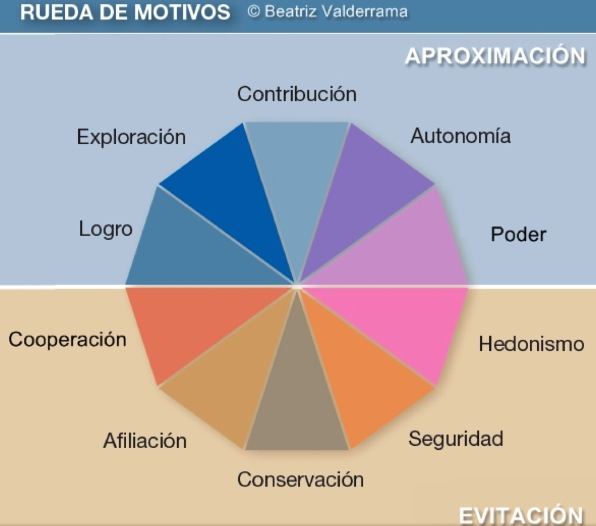
\includegraphics[width=0.5\textwidth]{imagenes\rueda-de-motivos}
\end{figure}

Es así como tenemos en contra partes diferentes motivos dependiendo del jugador obejtivo, que son la búsqueda de:
\begin{itemize}
	\item Logros o hedonismo
	\item Exploración o seguridad
	\item Contribución o conservación
	\item Autonomía o afiliación
	\item Poder o cooperación
\end{itemize}
 
%\subsection{Modelo de negocios en un videojuego}\label{modeloNegocio}
Para sustentar un proyecto o producto económicamente se debe tener claro un modelo de negocios. En el mundo de los videojuegos no existe la excepción, pero también debe considerarse que existen formas muy diferentes de adquirir el ingreso.

Incluso el mismo juego puede estar involucrado en un ingreso directo del servicio.

\subsubsection{Mercado global}
Se reporta segun Newzoo \cite{newzoo2018} que 2.3 billones de jugadores en todo el mundo gastarán \$ 137.9 billones en juegos en 2018. Esto representa un aumento de + 13.3\% en comparación con el año anterior, o \$ 16.2 billones. Los ingresos por juegos digitales tomarán el 91\% del mercado global con \$ 125.3 mil millones, como podemos ver en la \ref{fig:merglo}
\begin{figure}
	\centering
	\caption{Mércado global al primer trimestre del año 2018 por Newzoo \cite{newzoo2018}}
	\label{fig:merglo}
	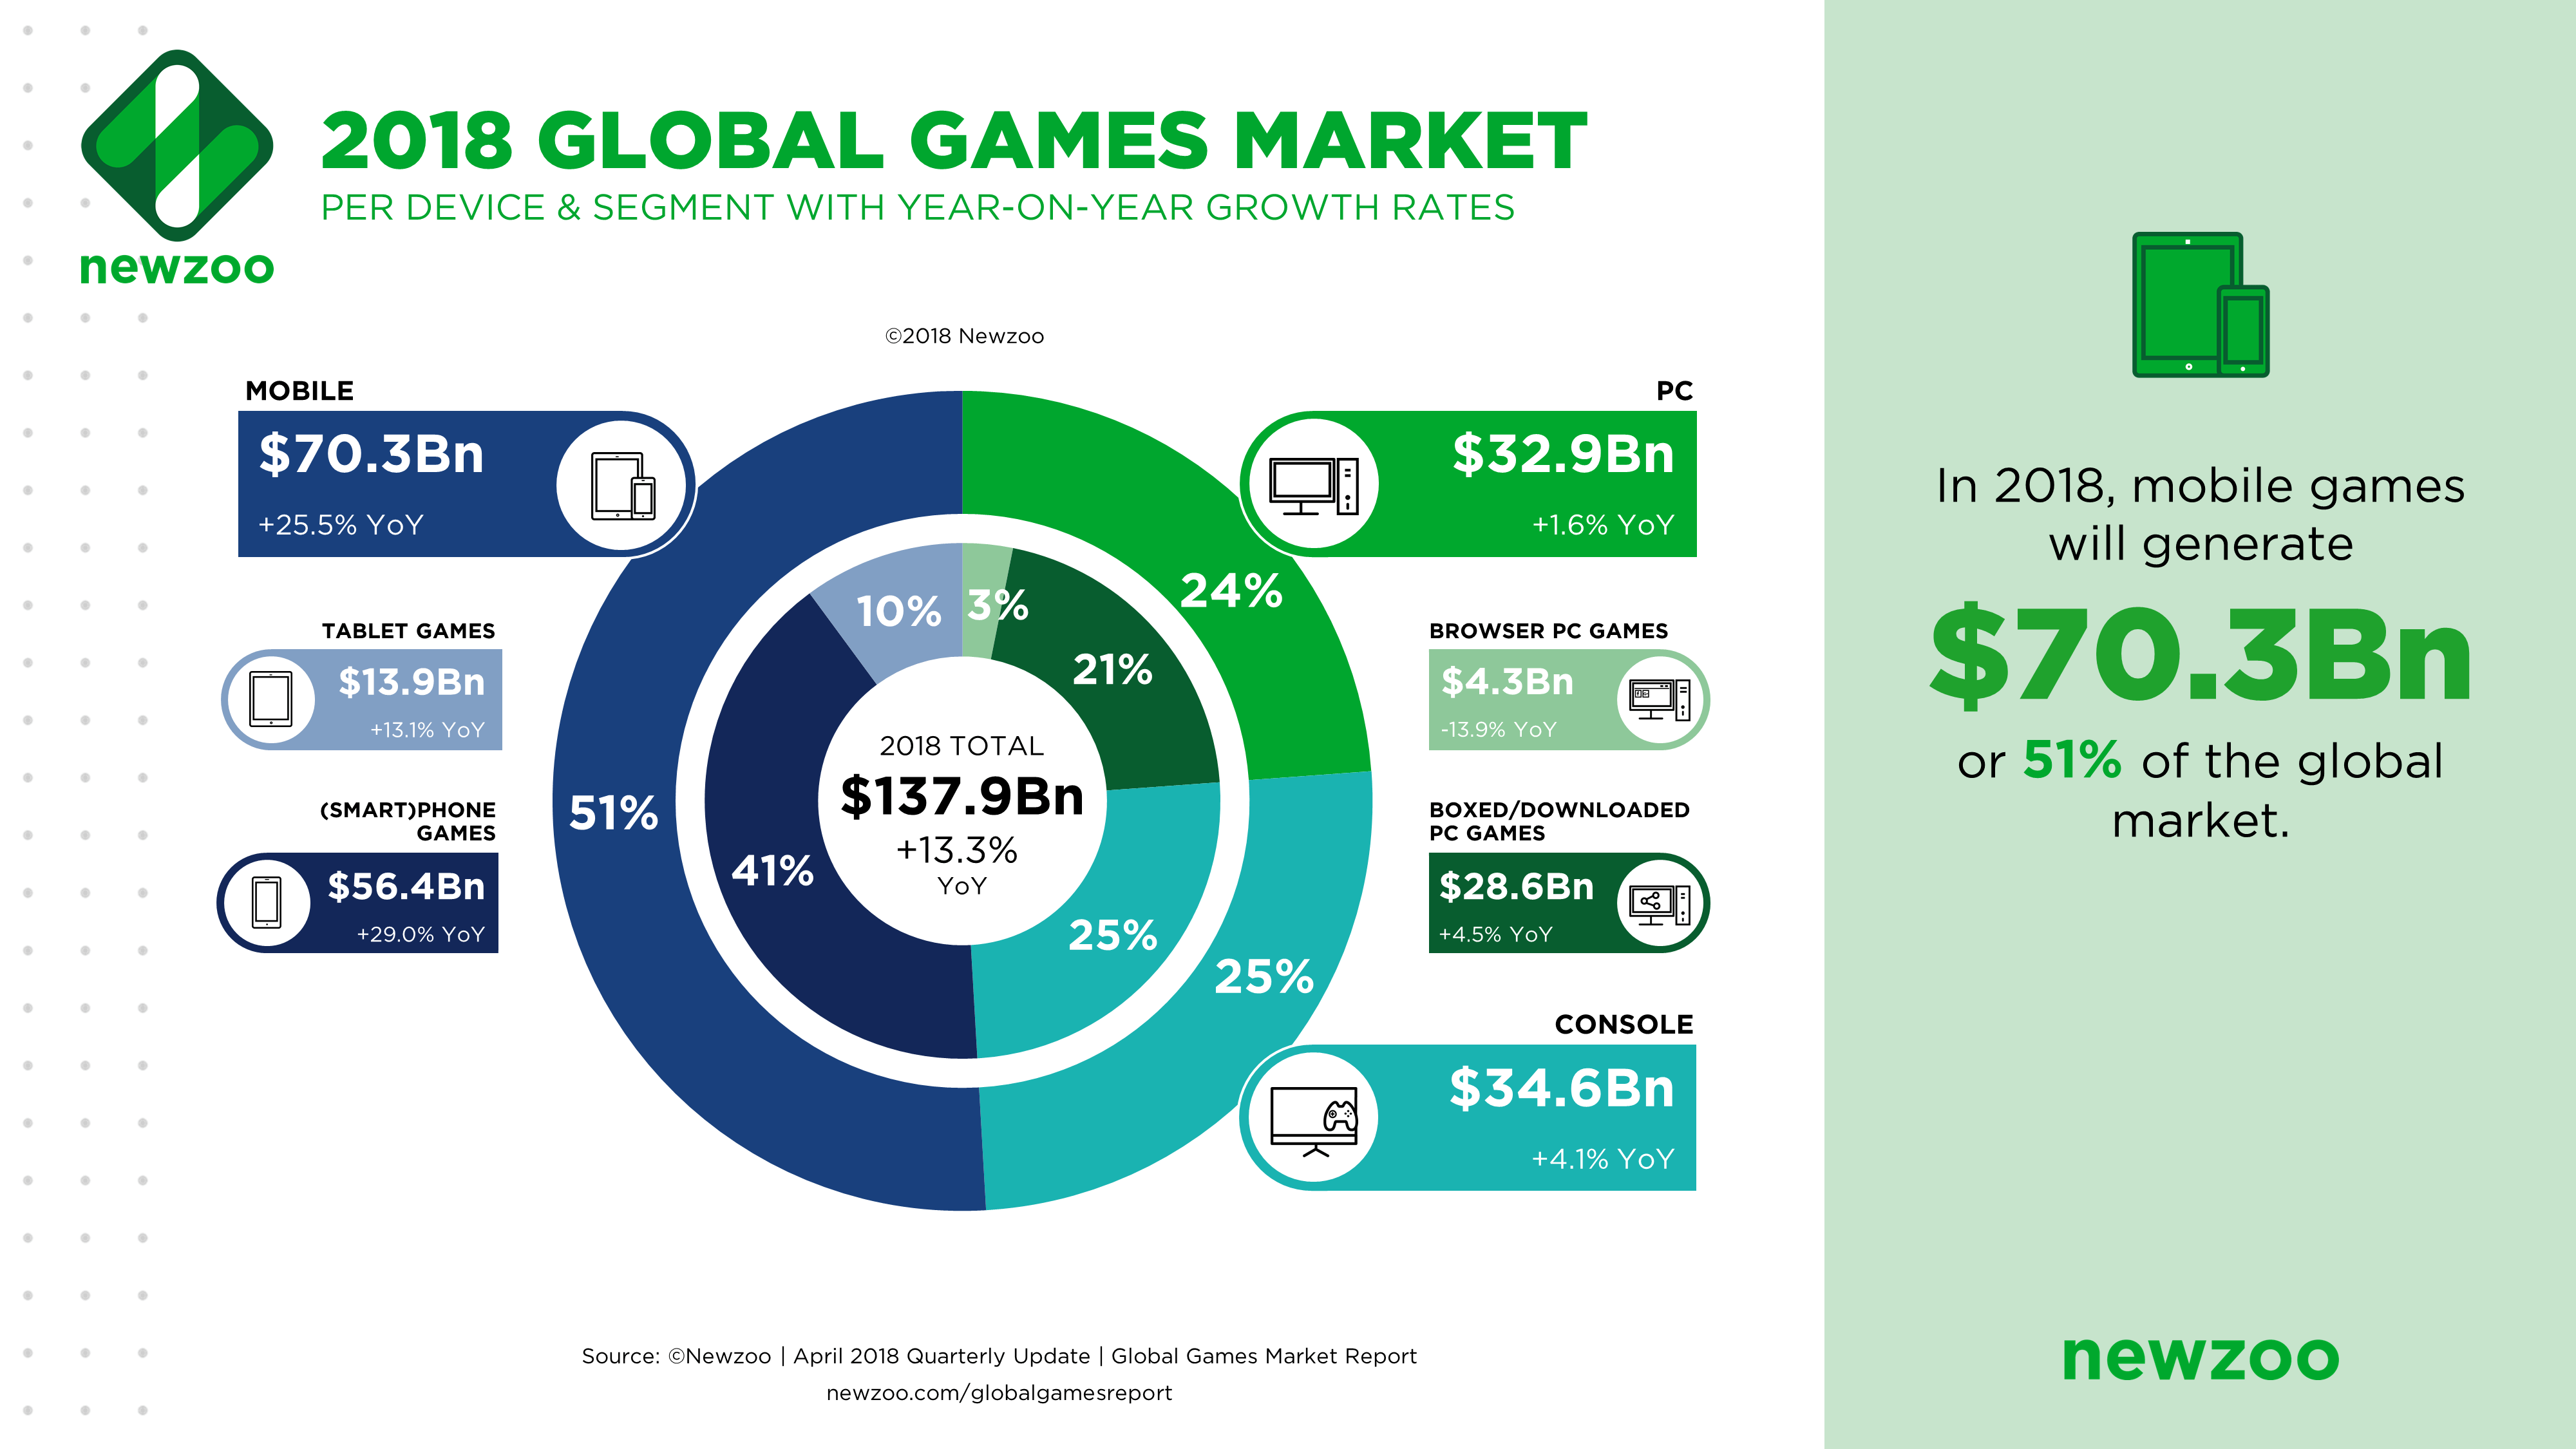
\includegraphics[width=0.5\textwidth]{02Antecedentes/contribucionesR/imagenes/merglo}
\end{figure}

Por primera vez, más de la mitad de todos los ingresos del juego provendrán del segmento móvil como vemos en la imagen{asdasd}. Los teléfonos inteligentes representarán el 80\% de esto, o \$ 56.4 mil millones, con el 20\% restante proveniente de tabletas.

\subsubsection{Salarios}
Para realizar un videojuego se necesita de diferentes profesiones para llevarlo a cabo.
En el siguiente cuadro \ref{tab:tablacostos} se mostrará la profesion y salario a recibir en la industria del videojuego en una empresa ya establecida al año 2014 segun la encuesta con una relación definida en experiencia.

% Please add the following required packages to your document preamble:
% \usepackage{multirow}
\begin{table}[htbp]
	\centering
\caption{Tabla de salarios dados en una empresa formal de videojuegos}
\label{tab:tablacostos}
\resizebox*{\linewidth}{!}{
	\begin{tabular}{|l|l|l|l|l|}
		\hline
		\textbf{Rama}                                                        & \textbf{Profesión}          & \textbf{Salario con -3años de exp.} & \textbf{Salario con 3-6años de exp.} & \textbf{Salario con +6años de exp.} \\ \hline
		\multirow{3}{*}{\textbf{Programadores e ingenieros}}                 & Programador                 & \$71,855 USD                        & \$79,877 USD                         & \$103,789 USD                       \\ \cline{2-5} 
		& Programador principal       &                                     & \$94,877 USD                         & \$116,151 USD                       \\ \cline{2-5} 
		& Director técnico            &                                     &                                      & \$135,781 USD                       \\ \hline
		\multirow{3}{*}{\textbf{Artistas y animadores}}                      & Animador                    & \$50,000 USD                        & \$55,547USD                          & \$82,230 USD                        \\ \cline{2-5} 
		& Artista principal           &                                     & \$71,029 USD                         & \$71,87576 USD                      \\ \cline{2-5} 
		& Director de arte            &                                     &                                      & \$110,000 USD                       \\ \hline
		\multicolumn{1}{|c|}{\multirow{2}{*}{\textbf{Diseñadores de juego}}} & Diseñador de juego          & \$53,000 USD                        & \$65,516 USD                         & \$77,768 USD                        \\ \cline{2-5} 
		\multicolumn{1}{|c|}{}                                               & Director creativo           &                                     & \$68,654 USD                         & \$101,944 USD                       \\ \hline
		\multicolumn{1}{|c|}{\multirow{3}{*}{\textbf{Productores}}}          & Productor asociado          &                                     & \$59,079 USD                         & \$61,912 USD                        \\ \cline{2-5} 
		\multicolumn{1}{|c|}{}                                               & Lider de proyecto           &                                     & \$73,500 USD                         & \$93,160 USD                        \\ \cline{2-5} 
		\multicolumn{1}{|c|}{}                                               & Productor ejecutivo         &                                     &                                      & \$126,833 USD                       \\ \hline
		\textbf{Profesional de audio}                                        & Director de sonido          &                                     &                                      & \$109,500 USD                       \\ \hline
		\multicolumn{1}{|c|}{\multirow{2}{*}{\textbf{Testers}}}              & Tester                      &                                     & \$38,833 USD                         &                                     \\ \cline{2-5} 
		\multicolumn{1}{|c|}{}                                               & Lider de control de calidad &                                     & \$60,417 USD                         & \$65,500 USD                        \\ \hline
		\multirow{3}{*}{\textbf{Negocios y administración}}                  & Marketing                   &                                     & \$73,500 USD                         &                                     \\ \cline{2-5} 
		& CEO                         &                                     &                                      & \$135,735 USD                       \\ \cline{2-5} 
		& Gerente ejecutivo           &                                     &                                      & \$156,731 USD                       \\ \hline
	\end{tabular}
}
\end{table}

\subsubsection{Presentación al cliente}
Un videojuego como cualquier software al momento de ser vendido al cliente puede encontrarse en dos presentaciones, una versión física o solo digital. En la siguiente tabla \ref{fiDi} se muestran las diferencias más destacables dadas por experiencia empresarial en el desarrollo por Velneo \cite{velneo2015}.

\begin{table}[htbp]
	\centering
	\caption{Tabla comparativa de un producto físico o digital por Velneo \cite{velneo2015}}
	\label{fiDi}
	\resizebox*{\linewidth}{!}{
\begin{tabular}{|l|l|l|}
	\hline
	\textbf{}                                             & \multicolumn{1}{c|}{\textbf{Físico}} & \multicolumn{1}{c|}{\textbf{Digital}} \\ \hline
	Coste de desarrollo                                   & sí                                   & sí                                    \\ \hline
	Coste de producción                                   & sí                                   & no                                    \\ \hline
	Coste de envío                                        & sí                                   & no                                    \\ \hline
	Riesgo de sobra/infra producir inventario             & sí                                   & no                                    \\ \hline
	Facturación por unidad vendida                        & mucho mayor                          & mucho menor                           \\ \hline
	Unidad vendida costea soporte                         & generalmente sí                      & imposible                             \\ \hline
	Porcentaje del precio de venta que percibe la empresa & 30\%-40\%                            & 70\%                                  \\ \hline
	Tiempo de cobro                                       & 90 días o más                        & 30 días                               \\ \hline
	Capacidad de llegar al público con marketing          & caro                                 & difícil                               \\ \hline
\end{tabular}
}
\end{table}

Aún así cabe mencionar que este es un aspecto general que involucra a cualquier software.

\subsubsection{Formas de ingreso}
Dentro de los videojuegos existen modelos de negocio que han dio cambiando a lo largo de los años y muchas de las veces depende del tipo del juego. Pero podemos definir las siguientes conforme lo visto y consumido en los últimos 5 años a la fecha del proyecto a presentar y con el apoyo de un artículo de la fundación UADE \cite{fundacionuade2014} en la tabla \ref{tablaMoneVJ}.

\begin{table}[htbp]
	\centering
	\caption{Tabla comparativa de ventajas y desventajas de modelos de negocios de videojuegos de autoría propia}
	\label{tablaMoneVJ}
	\resizebox*{\linewidth}{!}{
	\begin{tabular}{llll}
		Nombre       & Descripción                                                                                                               & Ventaja                                                                                                                                                                                                                                                                                                                  & Desventaja                                                                                                                                                                                                                                                                                                                                                                            \\
		Pay-to-play  & Se debe pagar contenido y uso del videojuego                                                                              & \begin{tabular}[c]{@{}l@{}}* Rápido retorno de inversión\\ \\ * Sin limitación de juego\\ \\ * Puede re-dirigirse a otro modelo en caso de fracaso \\ \\ * Puede ser un producto físico, por lo que puede cobrarse contenido extra\\ \\ * Complementa con compras in-game\end{tabular}                                   & \begin{tabular}[c]{@{}l@{}}* No compras por desconocimiento del juego (más en móviles)\\ \\ * Inversión grande por enfoque a consolas \\ \\ * Jugadores esperan contenido de entretenimiento de larga duración y calidad\\ \\ * No hay soporte o cambios en el juego\\ \\ * Si es un producto físico debe costearse la producción\\ \\ * Necesita publicidad\end{tabular}             \\
		Free-to-play & Ofrece gratis contenido y uso del videojuego en su totalidad, se monetiza con publicidad y compras in-game                & \begin{tabular}[c]{@{}l@{}}* Contacto con los jugadores más rápido\\ \\ * Preferente para móviles\\ \\ * Preferente para juegos de poca inversión (que quiera escalar)\\ \\ * Complementa con compras in-game\end{tabular}                                                                                               & \begin{tabular}[c]{@{}l@{}}* Depende de la cantidad de jugadores activos\\ \\ * Debe ser un juego con adicción para sustentarse\\ \\ * Debe ser un juego “infinito”\\ \\ * Requiere continuas actualizaciones si desea mantenerse\\ \\ * Debe darse al jugador contenido nuevo a jugar\end{tabular}                                                                                   \\
		Freemium     & Ofrece gratis el uso del videojuego pero no se accede a todo su contenido, establece jerarquización de tipos de jugadores & \begin{tabular}[c]{@{}l@{}}* Conveniente para demos (versión lite)\\ \\ * Oportunidad de dar a conocer el juego\\ \\ * Oportunidad de convencimiento al jugador\\ \\ * Contacto con los jugadores más rápido\\ \\ * Preferente para móviles\\ \\ * Viable aun sí existen pocos jugadores dispuestos a pagar\end{tabular} & \begin{tabular}[c]{@{}l@{}}* Debe crearse contenido de calidad por pago\\ \\ * Debe existir un control y registro de jugadores para su jerarquización\\ \\ * Usualmente el contenido extra debe ser descargado de internet (por lo que implicaría otros gastos y recursos)\\ \\ * Recomendable ser un juego “infinito”\\ \\ * A veces requiere continuas actualizaciones\end{tabular} \\
		Suscripción  & Se debe pagar el contenido y uso del videojuego pero con limitaciones.                                                    & \begin{tabular}[c]{@{}l@{}}* Es combinable con otros modelos como el freemium\\ \\ * Permite a los jugadores explorar el juego completo por cierto tiempo\\ \\ * Oportunidad de dar a conocer el juego\end{tabular}                                                                                                      & \begin{tabular}[c]{@{}l@{}}* Debe crearse contenido de calidad por pago\\ \\ * Recomendable ser un juego “infinito”\\ \\ * A veces requiere continuas actualizaciones\\ \\ * Debe darse al jugador contenido nuevo a jugar\\ \\ * Depende de la cantidad de jugadores activos\\ \\ * Debe ser un juego con adicción para sustentarse\end{tabular}         
	                           
	\end{tabular}
}
\end{table}



\subsubsection{Ingredientes de monetización}
Los modelos de negocio anteriores pueden ser combinables con otros "ingredientes" de monetización para acrecentarlos ingresos. 
\begin{itemize}
	\item Dinero virtual: Es el medio de intercambio que utiliza un videojuego para poder formalizar las compras dentro de él. A menudo se suele diferenciar el virtual currency (dinero virtual que se consigue por las propias mecánicas del juego y con abundancia) y el hard currency (dinero virtual premium que se consigue con dinero real o con acciones muy concretas y con mucha escasez).
	\item Bienes virtuales: Son objetos intangibles que son comprados e intercambiados que sólo tienen sentido dentro del juego, muchas veces estos son comprados con dinero virtual. 
	\item Publicidad y patrocinio: Anuncios o productos presentados en el juego para darse a conocer.
	\item Bonificaciones y servicios virtuales: Son aceleradores de juego o servicios que mejoran el desempeño o facilitan en el juego.
	\item DLC (downloadable content): Es un contenido de descarga digital exclusivo y adicional de un videojuego que se vende por separado y posterior al lanzamiento de este. Suele lanzarse para alargar la longevidad del videojuego y para aprovechar su éxito comercial. Su adquisición no tiene sentido sin tener antes el videojuego ya que es un producto complementario y dependiente a él.
\end{itemize}

%\subsection{Costo de hacer un videojuego}\label{costoVJ}

	
\subsubsection{Salarios}
Pararealizar un videojuego se necesita de diferentes profesiones parallevarlo a cabo.
En el siguiente cuadro se mostrará la profesion y salario a recibir en la industria del videojuego en una empresa ya establecida al año 2014 segun la encuesta ____ con una relación definida en experiencia.


\begin{table}[]
	\centering
	\caption{My caption}
	\label{my-label}
	\begin{tabular}{lllll}
		Rama                                                      & Profesión                   & Salario con \textless 3años de exp. & Salario con 3-6años de exp. & Salario con \textgreater 6años de exp. \\
		\multirow{3}{*}{Programadores e ingenieros}               & Programador                 & \$71,855 USD                        & \$79,877 USD                & \$103,789 USD                          \\
		& Programador principal       &                                     & \$94,877 USD                & \$116,151 USD                          \\
		& Director técnico            &                                     &                             & \$135,781 USD                          \\
		\multirow{3}{*}{Artistas y animadores}                    & Animador                    & \$50,000 USD                        & \$55,547USD                 & \$82,230 USD                           \\
		& Artista principal           &                                     & \$71,029 USD                & \$71,87576 USD                         \\
		& Director de arte            &                                     &                             & \$110,000 USD                          \\
		\multicolumn{1}{c}{\multirow{2}{*}{Diseñadores de juego}} & Diseñador de juego          & \$53,000 USD                        & \$65,516 USD                & \$77,768 USD                           \\
		\multicolumn{1}{c}{}                                      & Director creativo           &                                     & \$68,654 USD                & \$101,944 USD                          \\
		\multicolumn{1}{c}{\multirow{3}{*}{Productores}}          & Productor asociado          &                                     & \$59,079 USD                & \$61,912 USD                           \\
		\multicolumn{1}{c}{}                                      & Lider de proyecto           &                                     & \$73,500 USD                & \$93,160 USD                           \\
		\multicolumn{1}{c}{}                                      & Productor ejecutivo         &                                     &                             & \$126,833 USD                          \\
		Profesional de audio                                      & Director de sonido          &                                     &                             & \$109,500 USD                          \\
		\multicolumn{1}{c}{\multirow{2}{*}{Testers}}              & Tester                      &                                     & \$38,833 USD                &                                        \\
		\multicolumn{1}{c}{}                                      & Lider de control de calidad &                                     & \$60,417 USD                & \$65,500 USD                           \\
		\multirow{3}{*}{Negocios y administración}                & Marketing                   &                                     & \$73,500 USD                &                                        \\
		& CEO                         &                                     &                             & \$135,735 USD                          \\
		& Gerente ejecutivo           &                                     &                             & \$156,731 USD                         
	\end{tabular}
\end{table}

%\subsection{Vicio en el videojuego}\label{vicioVJ}
Un videojuego se está convirtiendo en una adicción cuando la ansiedad se sobrepone al placer del juego y como síntoma se tiene la urgencia de jugar sin pensar en las consecuencias. El vicio se establece con cierta facilidad, ya que el juego ofrece un entorno de inmersión al combinar los aspectos interactivos e identificarse con el personaje o situación.

En la siguiente tabla se muestra las opiniones más comunes a favor y en contra de los videojuegos sin incluir mitos o falsedades, todas estás afirmaciones son demostrables o no han sido posible desmentirlas con hechos o pruebas concretas.
\begin{table}[htbp]
	\centering
	\caption{Opiniones comunes a favor y en contra de los videojuegos}
	\label{tab:tablaOpinión}
	\begin{tabular}{ll}
		A favor                                                            & En contra                          \\
		Entretienen                                                        & Provocan adicción                  \\
		Ejercitan la coordinación óculo-manual                             & Promueven conductas violentas      \\
		Estimulan la capacidad de lógica y reflexión                       & Aíslan socialmente                 \\
		Ayudan a concentrar la atención                                    & Limitan la imaginación             \\
		Son un potencial muy adecuado para distintas aplicaciones sociales & Restan tiempo de otras actividades
	\end{tabular}
\end{table}
\\[1pt]
	
\subsubsection{Síntomas de vicio}
A continuación se muestran síntomas identificables visualmente que ya representan una adicción al juego:
\begin{itemize}
	\item El jugador parece estar absorto al juego, sin atender cuando lo llaman.
	\item Siente demasiada tensión, incluso aprieta las mandíbulas cuando juega.
	\item No aparta la vista de la pantalla.
	\item Empieza a perder interés por otras actividades que practicaba.
	\item Trastornos del sueño.
	\item Distanciamiento de familia y amigos.
	\item No respeta los horarios estipulados.
\end{itemize}


\subsubsection{Carcaterísticas de un videojuego con potencial al vicio}
Los videojuegos (en especial los free-to-play) contienen características de vicio como: la necesidad de concluir “tareas incompletas”, síntomas de abstinencia y la posibilidad de jugarlo en todo momento. En este apartado solo mencionaremos algunas de ellas y almenos las más visibles en muchos videojuegos.

 \begin{itemize}
 	\item El efecto Zeigarnik: Se tiene incomodidad de las personas por tener “tareas incompletas”, en el caso de un videojuego se genera la necesidad por terminar el juego. El juego a su vez puede contemplar el nivel de porcentaje completado de un juego, provocando al jugador dicho síntoma haciéndolo jugar hasta su completado.
 	
 	\item Síntoma de abstinencia: En donde se priva o dificulta la posibilidad de realizar una actividad a una persona. En un juego tenemos como se establece turnos de juego, para recuperarlos se establece un límite de tiempo de espera. Usualmente estos tiempos de espera son de aproximadamente media hora o múltiplos de ella, pues psicológicamente este tiempo es lo que soporta una persona con una “tarea incompleta” en mente.
 	
 	\item La competencia: Que consiste en una disputa entre personas que aspiran a un mismo objetivo o a la superioridad en algo. Así, en un juego, ayudado en la mayoría de las veces por las redes sociales se puede compartir y comparar el avance entre los jugadores.
 	 \\[1pt]
 	
 \end{itemize}

\subsubsection{Causas del vicio ajenas al videojuego }
Entre los jóvenes entre 13 y 18 años especialmente existen muchas más causas para caer en el vicio de un videojuego, pueden ser factores psicológicos, emocionales, del entorno en el que se desarrollan y más. Incluso muchos de los factores siguientes encajan en otros tipos de adicciones.
\begin{itemize}
	\item Atención inexistente de los padres.
	\item No hay límites establecidos por la familia.
	\item Los valores no están asentados.
	\item Utilización de los videojuegos como "niñera".
	\item El joven no tiene sentido de pertenencia o no es aceptado en los grupos sociales que interactúa.
	\item Necesidad de escape de la realidad a un medio virtual.
	\item Establece mayor libertad expresión (o intenciones verdaderas) dentro del juego, ya sean positivas o negativas.
	\item Que la persona padezca alguna enfermedad que imposibilite realizar otras actividades .
	\item Trastornos psicológicos como depresión, impulsividad o ansiedad.
	\item Situación ante la solución de problemas y toma de decisiones.
	\item Falta de control emocional.
\end{itemize}

\subsubsection{Prevención del vicio}
Como toda adicción existen formas de prevenir llegar a ella.
Dadas las situaciones, causas, factores dentro del vicio del videojuego y con lectura de técnicas pedagógicas, las propuestas de solución se dan como sigue:

\begin{itemize}
	\item Establecer un horario de juego:
	\begin{itemize}
		\item Se puede poner una alarma que avise al jugador que ha estado jugando demasiado tiempo.
		\item Se puede programar a cierto tiempo jugado un bloqueo.
	\end{itemize}
	\item Complementariamente a la programación de un horario de juego, deberán establecerse qué actividades se llevarán a cabo en los momentos en los que no se va a jugar:
	\begin{itemize}
		\item Poder agregar al juego notas recordatorias de las actividades por hacer.
		\item Alarmas personalizadas dentro del juego.
	\end{itemize}
	\item Evitar los juegos online, al menos hasta que se tenga una organización del tiempo libre que impida dedicar mucho tiempo a dichos videojuegos.
	\begin{itemize}
		\item Evitar ser un juego online.
	\end{itemize}
	\item  No instalar la consola ni el ordenador en la habitación.
	\begin{itemize}
		\item El juego va a ser inaccesible a horas determinadas como la madrugada y noche.
	\end{itemize}
	\item Los padres deben conocer los videojuegos.
	\begin{itemize}
		\item Pedir forzosamente los correos de los tutores.
		\item Mandar mensajes a los tutores con un registro en resumen de lo que se está jugando.
		\item Habilitar una opción de bloqueo para los padres.
		\item Bloqueo automático e informe con estadística dependiendo de frecuencia de uso y tiempo de uso.
	\end{itemize}
\end{itemize}


\section{Trabajo realizado durante trabajo terminal 1} \label{TrabajoTerminal1}
%\subsection{Presentado en TT1}\label{tt1}
A continuación se muestra lo presentado en TT1, que representa la investigación, análisis y prototipos del proyecto.

\subsubsection{Contexto}\label{contexto}
Primero nos encontramos a determinar que es la cultura; aquella que define la identidad de un individuo por sus creencias religiosas, de pensamiento, sentimentales y sociales. Mientras que la historia son todos los sucesos pasados dentro de un espacio específico. Entonces la cultura histórica es aquellos aspectos arquitectónicos, de pensamiento, éticas y morales, grupos de pertenencia y convivencia. Dentro de la hultura histórica encontramos que el 41\% de los mexicanos no asisten a eventos culturales y presentan una gran desinformación de ella.

Luego nos encontramos que existen formas de presentar cualquier tema o actividad dentro de los juegos. A partir de eso investigamos sobre los videojuegos, juegos que se presentan a través de un medio visiual o auditivo en el que existe interacción por diferentes dispositivos de entrada. Dentro de los videojuegos hay clasificaciones por contenido, que son las utilizadas para determinar el tipo de público al que va dirigido, además de que es una clasificación conveniente para limitar compra y venta. Sin embargo existen muchas más clasificaciones, en donde el tipo de contenido, dispositivo u objetivo es su pertenencia.

\subsubsection{Viabilidad}\label{viabilidad}
Con esta información ya en mano, buscamos sobre la situación actual de comercio de los videojuegos. Pasando primero por los ingresos a nivel mundial y en que dispositvos en el año 2017; a nivel mundial se tiene un ingreso de \$108.9 mil millones de dolares, el 42\% está en los dispositvos móviles, tanto teléfonos inteligentes como tabletas, el resto queda en la computadora y consolas. Así México queda en el doceavo lugar de consumo de videojuegos a nivel mundial, con un ingreso percibido de \$1.4 mil millones de dolares en una población de 130 millones de mexicanos. De la población en México el 20\% juega videojuegos, de ese porcentaje 45\% juega en el celular y 40\% juega de una a dos veces por semana.

\subsubsection{Análisis}\label{analisis}
Una vez contemplada la información, se decide que el proyecto se haga en un dispositvo móvil android, dado que el 86\% de los usuarios de dispositivos móviles tienen android y como versión mínima 5.0 lolipop con su uso de 32\% de las personas.

La metodología a usar será Hundle, que consiste en un parecido a la metología scrum solo que está adaptada a la creación y desarrollo de videojuegos, donde se establece un proceso general de preproducción,  producción y postmortem. Destacando aquí que se hicieron algunos ajustes dentro de la parte de preproducción agregando y modificando apartados daddo que eran necesarios aclarar antes de empezar con el proyecto.

Luego se pasó a definir las herramientas de desarrollo, donde se escogió debido a su flexibilidad multiplataforma el motor de juego Unity y como herramientas de dibujo corel draw x5 y photoshop.

Como arquitectura a usar se eligió modelo vista controlador, donde se dividirá el código en controladores, actores y auxiliares, estos últimos ayudarán a los controladores y actores en situaciones específicas donde no se encuentre en ninguna de estas características.

\subsubsection{Progresión y prototipos}\label{proypro}
Ya realizadas las investigaciones y análisis previo para el proyecto, se estableció la progresión que iba a tener el juego, junto con definir las interfaces que contendría y su interacción entre ellas.
Se estableció la mecánica del juego donde se definía los botones de acción del personaje, el espacio de características del personaje y un apartado para determinar otros factores como items o vida del enemigo.

Ya en los prototipos se pasó a el maquetado de los niveles uno y dos, determinando personajes y eventos, así como prototipos de uso de la herramienta Unity.Al final dando como resultado dos prototipos conteniendo el nivel uno y dos y un prototipo de uso de la herramienta.

En esta sección se habla a manera de resumen el trabajo realizado durante el 
periodo correspondiente a trabajo terminal 1. La división de esta sección 
queda organizada en dos subsecciónes: una para la etapa de preprodución y 
otra para los dos primeros \textit{sprints} de la estapa de produción. 

\subsection{Etapa de Preproducción}\label{EtapaPreproduccion}
Esta etapa corresponde a la planeación analisis y diseño del juego. Como lo indica 
la metodología \textit{Huddle}, para esta etapa se trabaja en el desarrollo del 
documento de diseño del juego. Esta etapa queda del desarrollo queda dividida en 
cuatro \textit{sprints}.

\subsubsection{Primer Sprint Huddle de Preproducción}\label{Prepro01}
Antes de iniciar el diseño del juego se realiza un trabajo de investigación 
sobre la cultura azteca. Esta investigación abarca:
\begin{itemize}
        \item \textbf{La sociedad mexica:} su historia tradiciones y clases sociales. 
        \item \textbf{Mitología mexica:} Dioses, mito de los cinco soles, mito de la 
        creación del hombre del maíz, el Mictlán.
        \item \textbf{Historia de la Malinche:} Historia del personaje antes y después 
        de la llegada de los españoles.
\end{itemize} 
 
Durante la etapa de investigación se selecciona la información histórica que 
sera relevante y útil para la narrativa del juego y el diseño de su jugabilidad. 
Para la investigación histórica de esta etapa se consultan libros, códices, 
páginas de Internet, artículos de investigación e incluso se visitan museos 
como el templo mayor.

\subsubsection{Segundo Sprint Huddle de Preproducción}\label{PrePro02}
En este \textit{sprint} se redactan las primeras secciones del documento de diseño del 
juego \textit{Yolotl}. Se inicia con la idea concepto y con el tema del juego. De igual 
forma se selecciona un nombre para el juego a desarrollar: \textit{Yolotl}. 
Para algunos juegos la mecánica es la primera es ser definida; no obstante, 
por la naturaleza del juego como herramienta de transmisión de cultura, 
\textit{Yolotl} nace con su historia. La historia de \textit{Yolotl} pasa por 
diferentes etapas de diseño; siendo modificada gradualmente, pero manteniendo 
algunos elementos clave como la lucha contra la divinidad. 
\\
\par
En la etapa del concepto también se define la plataforma para la que será 
el juego: dispositivos móviles con sistema operativo Android 5.2. Por su parte 
se decide utilizar un motor de juego como herramienta de desarrollo, pues esto 
permite centrarse en el diseño e implementación de aquellos elementos que 
diferencien a \textit{Yolotl} del resto de juegos, tal como su mecánica, sus 
personajes, etc. Luego de investigar sobre los motores de juegos disponibles, 
se elije Unity 3D como ambiente de desarrollo.
\\
\par
Una vez teniendo la idea concepto se define la visión del juego y sus mecánicas. 
En cuestión de las mecánicas el enfoque por el que se opta es el de mantener 
el juego con mecánicas simples y familiares para aquellos jugadores que ya habían 
tenido alguna experiencia con algún juego de plataformas, sin descartar algunos 
detalles que le dieran identidad al juego en cuanto a su jugabilidad. Paralelamente 
a la preproducción, se inicia el desarrollo de un primer demo con el fin de 
familiarizarse con la herramienta de Unity3D, este demo incluye las mecánicas más 
simples del juego.
\\
\par
Con la historia, la visión y la mecánica definidas se procede a puntualizar los 
estados del juego, diseñar las interfaces gráficas de navegación y de interacción 
con el personaje. Para ver la versión final de las interfaces se puede consultar 
anexo \ref{Anexo:Intefaces}.

\subsubsection{Tercer Sprint Huddle de Preproducción}
En el tercer Sprint se definen la cantidad de niveles y en que consiste
cada uno, de igual forma se establecen los objetivos de cada nivel, la recompensa 
a obtener una vez completado el mismo, los enemigos a vencer y las cinemáticas que 
fungen como transiciones entre niveles.  
\\
\par
Al mismo tiempo que se diseñan los niveles, se detallan los 
personajes tanto a nivel narrativo como a nivel de jugabilidad, definiendo habilidades 
para los enemigos, los niveles en los que parecerían y sus acciones dentro de 
la historia. Para esta parte se trata de obtener la mayor fidelidad posible a 
los mitos y códices. En el anexo \ref{Anexo:Personajes} se habla a mayor detalle 
sobre el diseño de los personajes.

\subsubsection{Cuarto Sprint Huddle de Preproducción} 
En el cuarto sprint se termina de escribir el argumento del juego, de esta 
destapa se obtiene el guión literario del juego. En este \textit{sprint} también se definen 
elementos de ambientación para el juego tales como la música de fondo, los 
efectos de sonido y los efectos especiales. 
\\
\par
De igual forma, en este \textit{sprint} se especifican las armas de los personajes, los 
ítems; quedando diseñados tanto a nivel de comportamiento como a nivel 
visual. Al igual que con los personajes se busca que las armas, tanto en 
comportamiento como en diseño, se mantengan lo más fiel posible a los mitos 
y leyendas de donde se basaron.
\\
\par
Con el cuarto \textit{sprint} se finaliza la etapa de preproducción, obteniendo así un 
documento de diseño lo suficientemente detallado como para iniciar el diseño 
del juego a nivel de ingeniera. 

\subsection{Etapa de producción}
En esta sección se habla del trabajo realizado durante los dos primeros 
\textit{sprints} de esta etapa, ya que fueron desarrollados durante los meses 
correspondientes al trabajo terminal 1. Todos los \textit{sprints} del la etapa 
de producción posteriores al segundo \textit{sprint} son abordados en la sección 
\ref{TrabajoTT2}.

\subsubsection{Primer Sprint Huddle de Producción.}
En este \textit{sprint} se realiza un análisis del documento de diseño, en consecuencia 
de este análisis se se diseña el videojuego en materia de las clases que lo 
componen y el modelo bajo el que funcionaría el juego a nivel de programación. 
\\
\par
Haciendo uso del paradigma orientado a objetos se propone emplear tres tipos 
de clases:
\begin{itemize}
        \item \textbf{Actores:} Son las clases que modelan a los enemigos, los ítems, 
        los coleccionables, los checkpoints y al jugador.
        \item \textbf{Controladores:} Son las clases encargadas de gestionar la partida 
        y la navegación entre interfaces. Estas clases desencadenan eventos conforme a 
        las acciones de las clases actoras. Estas clases también son las encargadas de 
        verificar que se cumplan las reglas de los niveles.
        \item \textbf{Auxiliares:} Estas clases ayudan al funcionamiento de los actores 
        y los controladores. Estas clases también se encargan le vincular datos con 
        las clases controladoras como efectos de sonido, música, datos para la 
        progresión entre niveles.
\end{itemize}
El modelo planteado permite reutilizar parte del demo generado durante la etapa 
de preproducción. Por lo aque en este \textit{sprint} se inicia la integración 
del código del primer demo con el comportamiento modelado por las clases definidas 
en el párrafo anterior. 
\\
\par
En el primer \textit{sprint} de Producción también se crean los \textit{sprites} del 
primer nivel utilizando la herramienta de modelado en \textit{3D Blender}. En la
figura \ref{fig:Modelos3D} se pueden observar algunos de los modelos creados. Al 
finalizar este \textit{sprint} se determina la no viabilidad del modelado en 3D de los 
\textit{sprites} por cuestiones de tiempos; en consecuencia, se descarta este 
método para generar los \textit{sprites} y se inicia el desarrollo de los 
\textit{sprites} a partir de otras técnicas de animación más tradicionales.

\begin{figure}[h]
  		\centering
   		\subfigure[Modelo de \textit{Malinalli} generado en \textit{Blender}.] {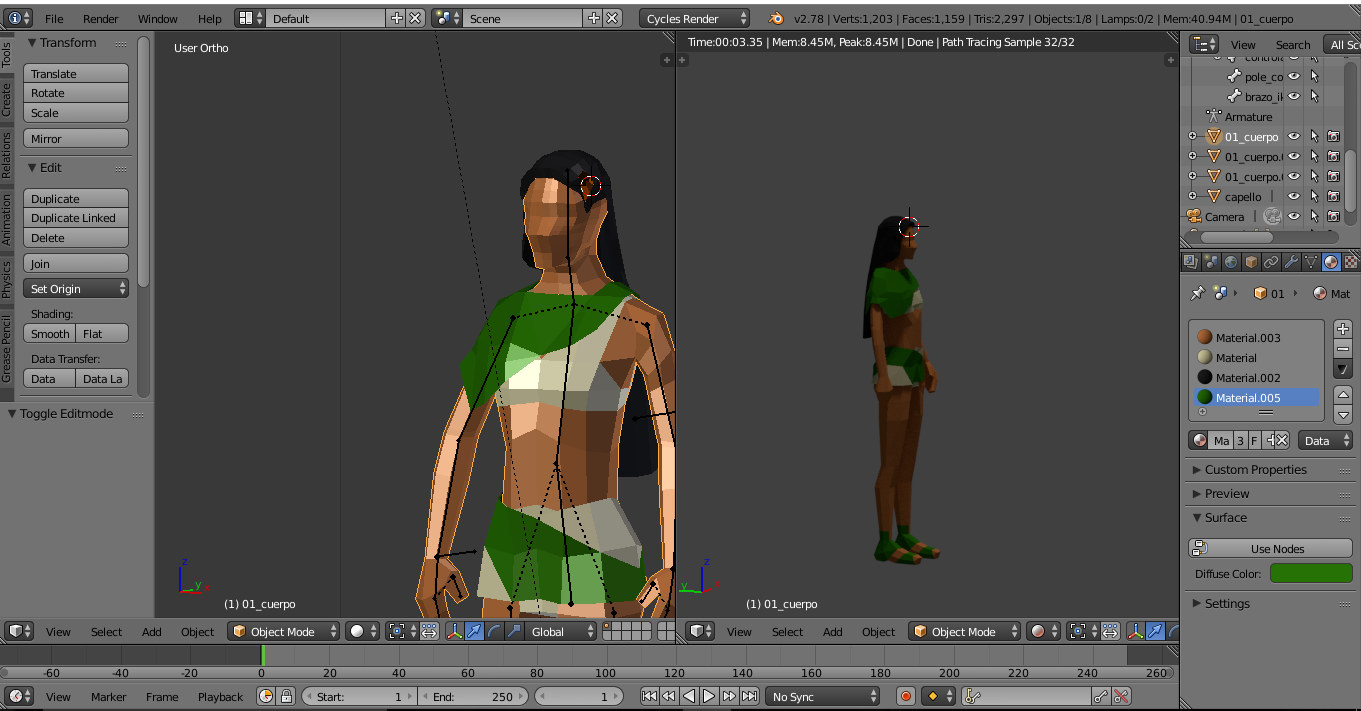
\includegraphics[width=0.3 \textwidth]{02Antecedentes/Imagenes/Malinalli_proceso.png}}
   
 		\subfigure[Modelo de \textit{Xólotl} generado en \textit{Blender}.]{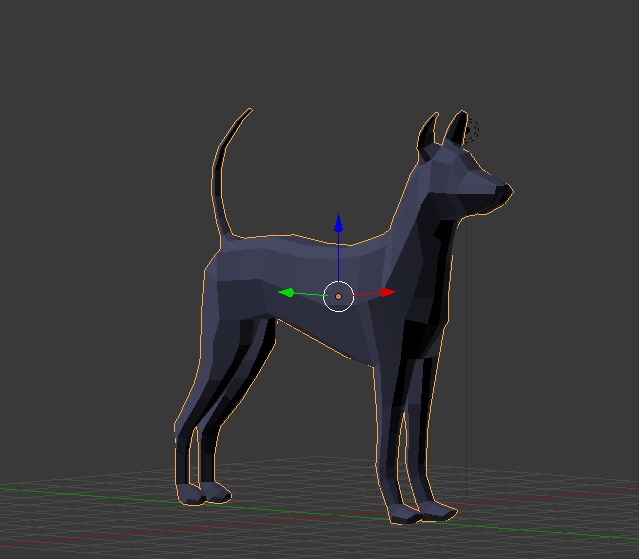
\includegraphics[width=0.3 \textwidth]{02Antecedentes/Imagenes/xolo.jpg}}
 	
		\subfigure[Modelo de un templo generado en \textit{Blender}.] {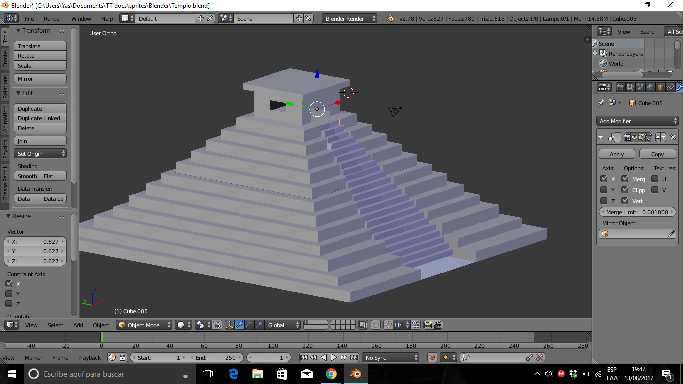
\includegraphics[width=0.3 \textwidth]{02Antecedentes/Imagenes/templo.png}}
		
		\subfigure[Modelo de una mujer comerciante generado en \textit{Blender}.] {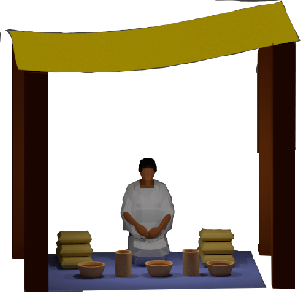
\includegraphics[width=0.3 \textwidth]{02Antecedentes/Imagenes/Mujer04_game.png}}
		
  		\caption{Modelos de personajes y objetos crados en \textit{Blender} (Autoria propia).}
  		\label{fig:Modelos3D}
\end{figure}

\subsubsection{Segundo Sprint Huddle de Producción.}
En este \textit{sprint} se inicia el desarrollo de los \textit{sprites} 
con \textit{Adobe Photoshop} y \textit{Corel Draw}. A la par se inicia la 
maquetación de la etapa de selva del nivel uno. En este sprint se logran 
terminar todos los \textit{sprites} referentes al primer nivel del juego 
tales como: 

\begin{itemize}
        \item Objetos de fondo: Arbustos, árboles, jarrones y cajas. 
        \item Imagen de fondo: Fondo de la selva, la ciudad y el menú principal. 
        \item Ciudadanos del mercado: Comerciantes, nobles y esclavos. 
        \item \textit{Xólotl} en su forma \textit{xoloitzcuintle}: Bloques de 
        animacion para correr y normal.
        \item \textit{Malinalli} sin la caracola: Bloques de animación correr, 
        saltar y normal.
\end{itemize}
Una vez terminados los \textit{sprites} referentes al nivel uno estos se integran al código 
permitiendo tener un segundo prototipo con la siguiente funcionalidad:
\begin{itemize}
        \item Control de personaje por medio de la GUI.
        \item Transiciones entre interfaces.
        \item Personaje seguible que aparece en el primer nivel funcional.
        \item Funcionamiento básico del controlador de diálogos.
\end{itemize}


	\chapter{Trabajo realizado} \label{TrabajoTT2}
En este capítulo se habla de los \textit{sprints} de la etapa de producción que
abarcan el trabajo terminal 2, es decir los \textit{sprints} del tres al diez. El
onceavo \textit{sprint} no es abarcado en este capítulo ya que de él se habla en la
sección correspondiente a la pruebas. Cada \textit{sprint} es abordado mencionando
primeramente su objetivo, después se describe todo lo realizado durante el
\textit{sprint} y se finaliza mencionando si se completo el \textit{sprint} y que
se obtuvo al final del mismo. Es importante recalcar que los \textit{sprints} se
abordan en este capítulo de manera secuencial, sin embargo los \textit{sprints}
impares corresponden al desarrollo de los niveles impares, mientras que los pares
corresponden al desarrollo de los niveles pares; esto debido a la nueva asignación
de trabajo, ver sección \ref{Sec:AsignacionTrabajo}.

%\subsection{Detalles del proyecto}
Aquí se mostrará del proyecto el título, estudio, género, plataforma, fecha de inicio, fecha de término, lo planeado, en desarrollo, sin planear y terminado.
\\
\subsubsection{Título}
Yolotl

\subsubsection{Estudio}
ESCOM - IPN

\subsubsection{Plataforma}
Dispositivos móviles android

\subsubsection{Fecha de inicio}
1 Agosto 2017

\subsubsection{Fecha de término}
1 Junio 2018
\subsubsection{Planeado}
El 80\%
\subsubsection{Desarrollo}
El 10\%
\subsubsection{Planear}
El 20\%
\subsubsection{Terminado}
El 0\%



\subsection{Sprint plan 1}
\subsubsection{SprintID}
01
\subsubsection{Inicio}
1 Agosto 2017
\subsubsection{Fin}
31 Agosto 2017
\subsubsection{Meta}
Nivel 1
\subsubsection{Porcentaje}
El 16\% 


\subsubsection{FeatureID}
01
\subsubsection{Nombre}
N1
\subsubsection{Estado}
Planeado

\subsubsection{SprintID}
01
\subsubsection{Comentarios}
-


\subsection{Sprint backlog 1}
\subsubsection{Sprint backlog}
01

\subsubsection{Tareas}
6
\subsubsection{Tendencia}
0
\subsubsection{Esfuerzo restante}
56
\subsubsection{Tendencia actual}
-
\subsubsection{Progreso ideal}
10
\subsubsection{Tareas restantes}
10
\subsubsection{Nombre de la tarea}
n1
\subsubsection{FeatureID}
01
\subsubsection{Miembro}
Rocío
\subsubsection{Rol}
Desarrollo
\subsubsection{Estado}
Planeado
\subsubsection{Esfuerzo}
10
\subsection{Buglist}
\subsubsection{BugID}
01
\subsubsection{Descripción}
Doble salto infinito
\subsubsection{Descripción técnica}
El gameobject no realiza la función detectar colisión de el "piso" 
\subsubsection{Autor}
Velez
\subsubsection{Estado}
Revisión
\subsubsection{FeatureID}
01


\subsection{Task Slips 1}


\subsubsection{FeatureID}1
\subsubsection{Nombre}Maqueta
\subsubsection{Tarea}Realizar maqueta del nivel completo
\subsubsection{Miembro}Rocío
\subsubsection{Esfuerzo estimado}1
\subsubsection{Terminado}si
\subsubsection{Restante}0


\subsubsection{FeatureID} 1
\subsubsection{Nombre} Enemigos
\subsubsection{Tarea} Realizar el comportamiento de los enemigos o cualquier otra acción necesaria dentro del nivel
\subsubsection{Miembro} Rocio
\subsubsection{Esfuerzo estimado} 3
\subsubsection{Terminado} sí
\subsubsection{Restante} 0


\subsubsection{FeatureID} 1
\subsubsection{Nombre} Arte 1
\subsubsection{Tarea} Crear vista de los personajes
\subsubsection{Miembro} Rocío
\subsubsection{Esfuerzo estimado} 2
\subsubsection{Terminado} sí
\subsubsection{Restante} 0



\subsubsection{FeatureID} 1
\subsubsection{Nombre} Arte 2
\subsubsection{Tarea} Crear el diseño de los obstáculos
\subsubsection{Miembro} Rocío
\subsubsection{Esfuerzo estimado} 2
\subsubsection{Terminado} sí
\subsubsection{Restante} 0


\subsubsection{FeatureID} 1
\subsubsection{Nombre} Arte 3
\subsubsection{Tarea} Crear el diseño de los items
\subsubsection{Miembro} Rocio
\subsubsection{Esfuerzo estimado} 2
\subsubsection{Terminado} sí
\subsubsection{Restante} 0


\section{Tercer sprint de producción}
Esta etapa contiene el desarrollo del nivel tres del juego. El panorama general abarca un nivel de manera ascendente en un terreno rocoso. Después se llega al jefe que tiene forma de jaguar Tepeyóllotl.

Primero se empieza con el maquetado del nivel, para establecer el tamaño del nivel, pues esta vez será de manera vertical el diseño, y la cámara solo se moverá en esa dirección. Se establece también donde debe ir cada objeto o enemigo junto con anotaciones necesarias para la comprensión posterior, como son direcciones de movimiento o acciones que deben realizarse. Aquí se debe tomar muy en cuenta el tamaño del personaje a jugar si no, no se podrá avanzar en el nivel ya que se da la situación a atorarse debido al tamaño, incluido el espacio para saltar. Lo anterior se puede ver en la figura \ref{fig:n01}.
\begin{figure}[htbp]
	\centering
	\subfigure[Primera parte del nivel]{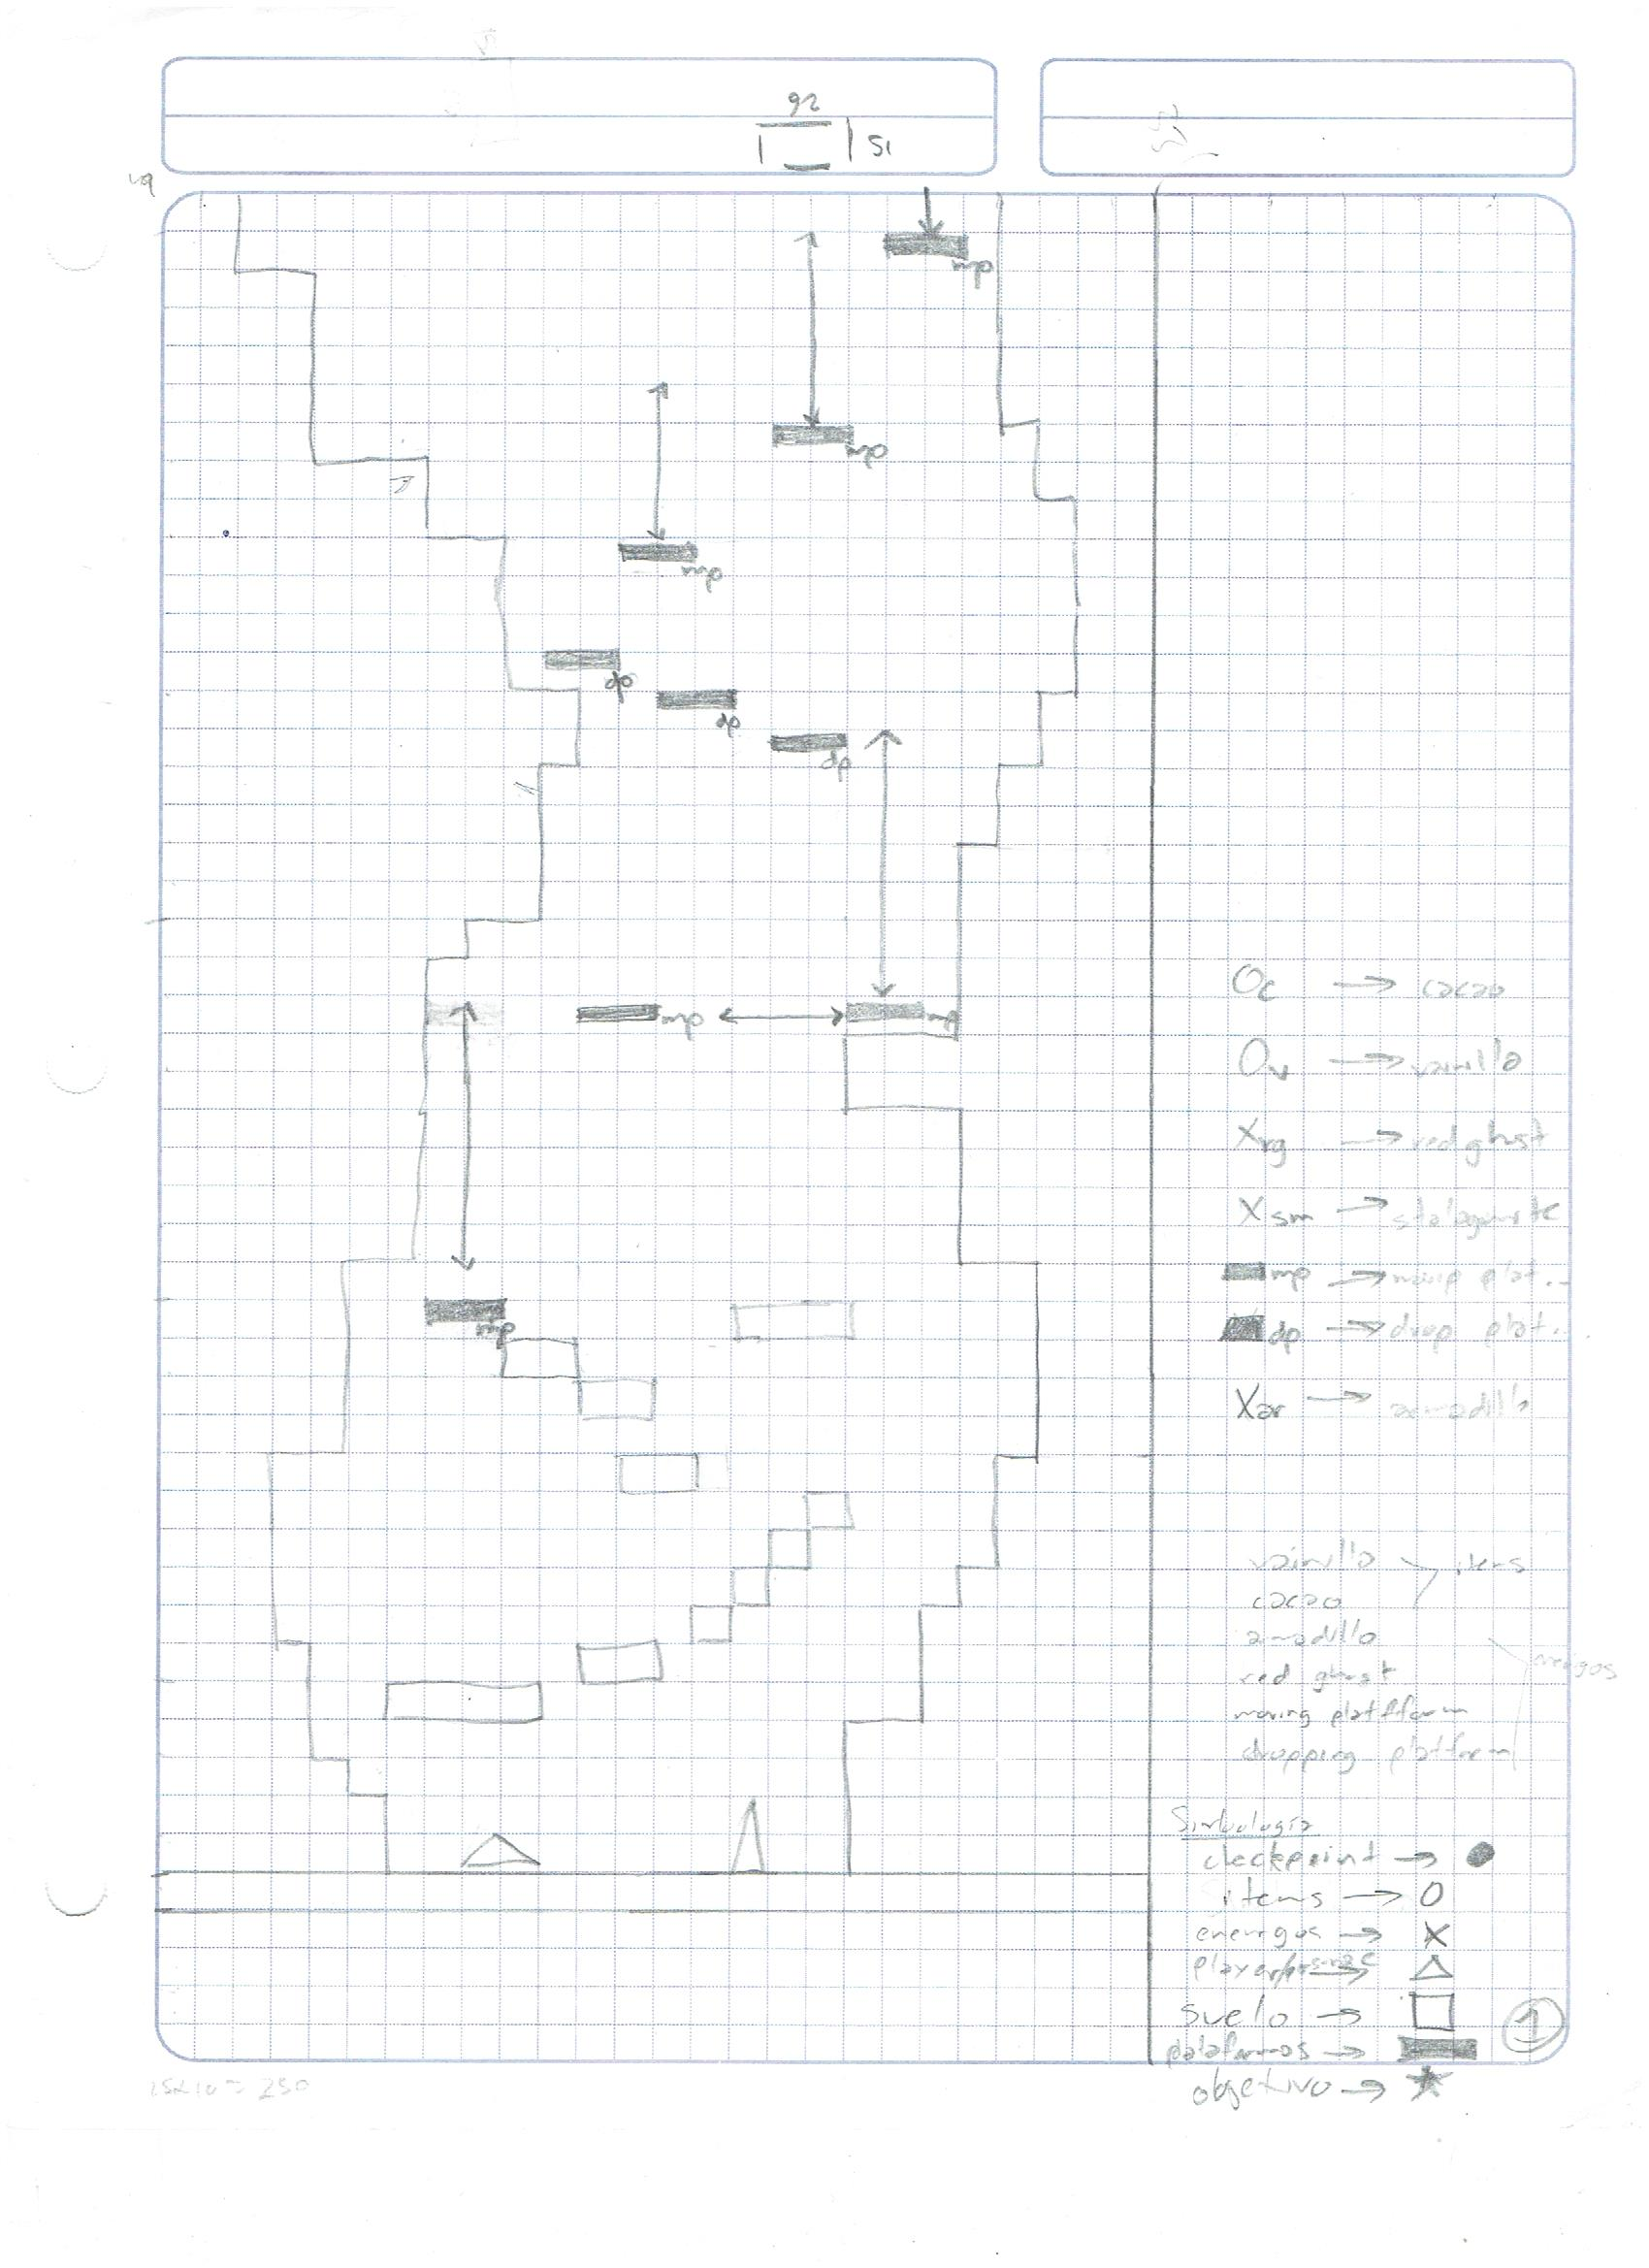
\includegraphics[width=5cm]{03TrabajoRealizado/DocProduccionR/imagenes/n3/01.jpg}}
	\subfigure[Segunda parte del nivel]{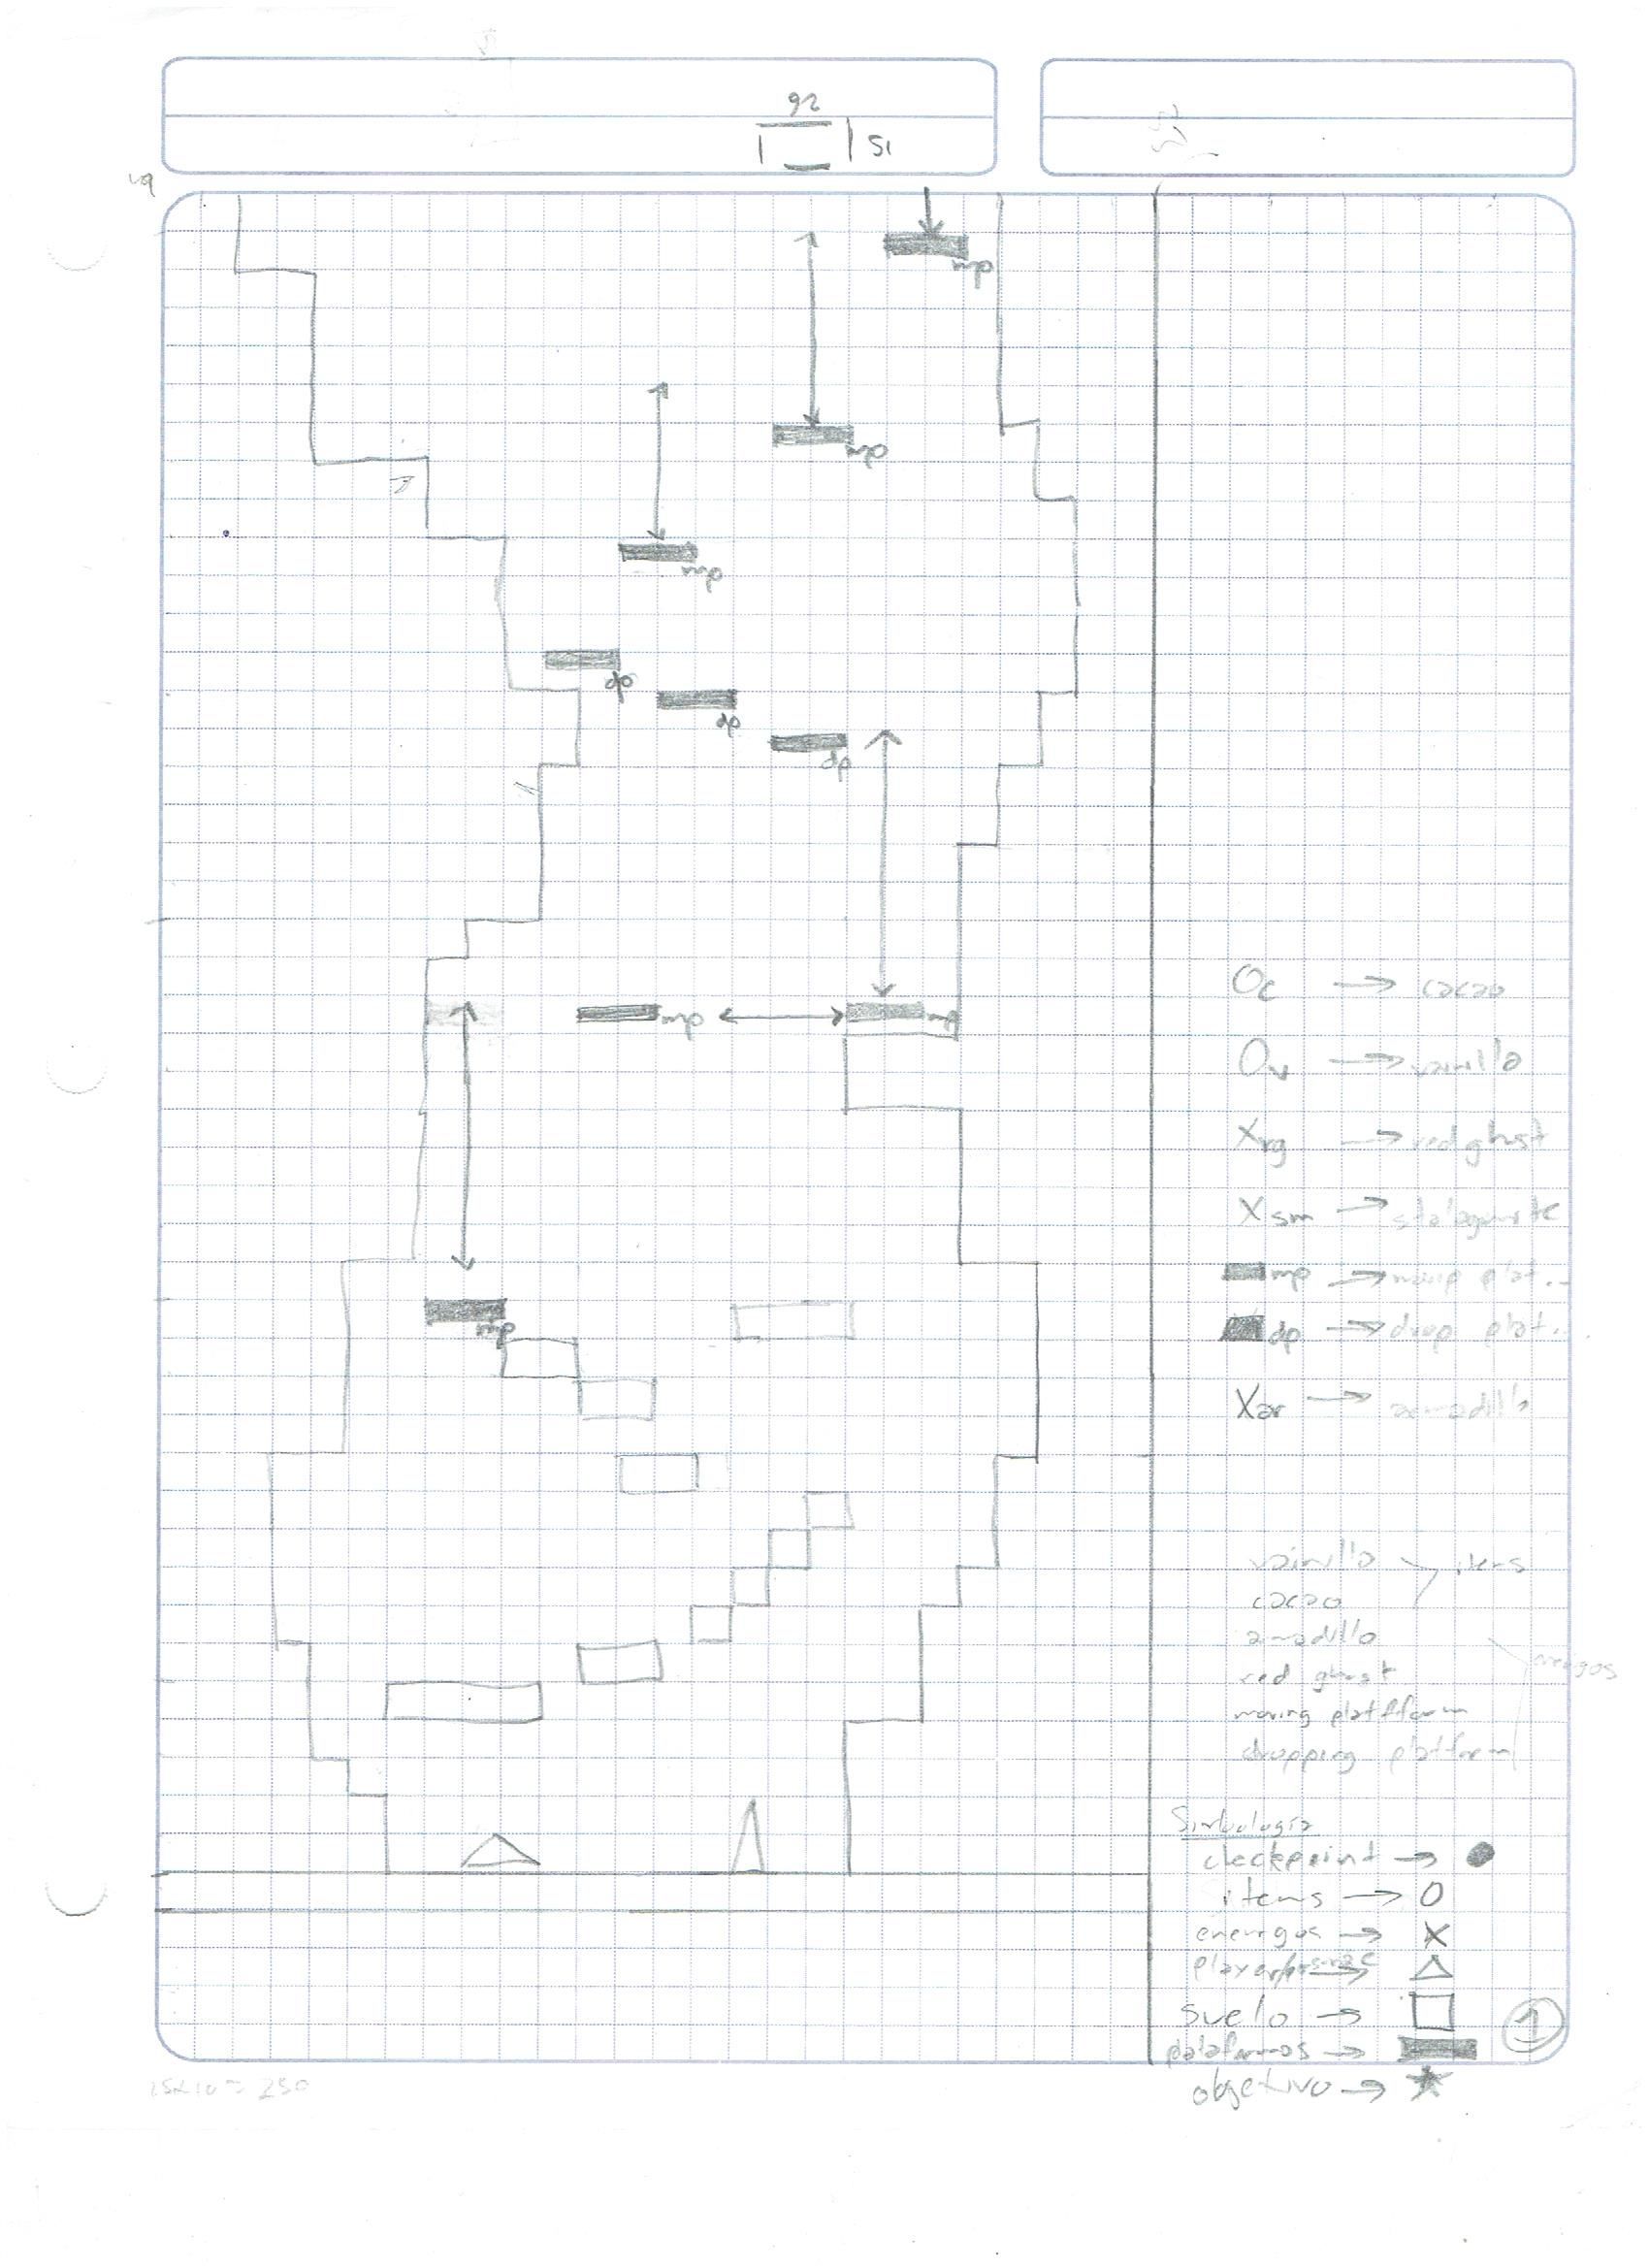
\includegraphics[width=5cm]{03TrabajoRealizado/DocProduccionR/imagenes/n3/02.jpg}}
	\subfigure[Tercera parte del nivel]{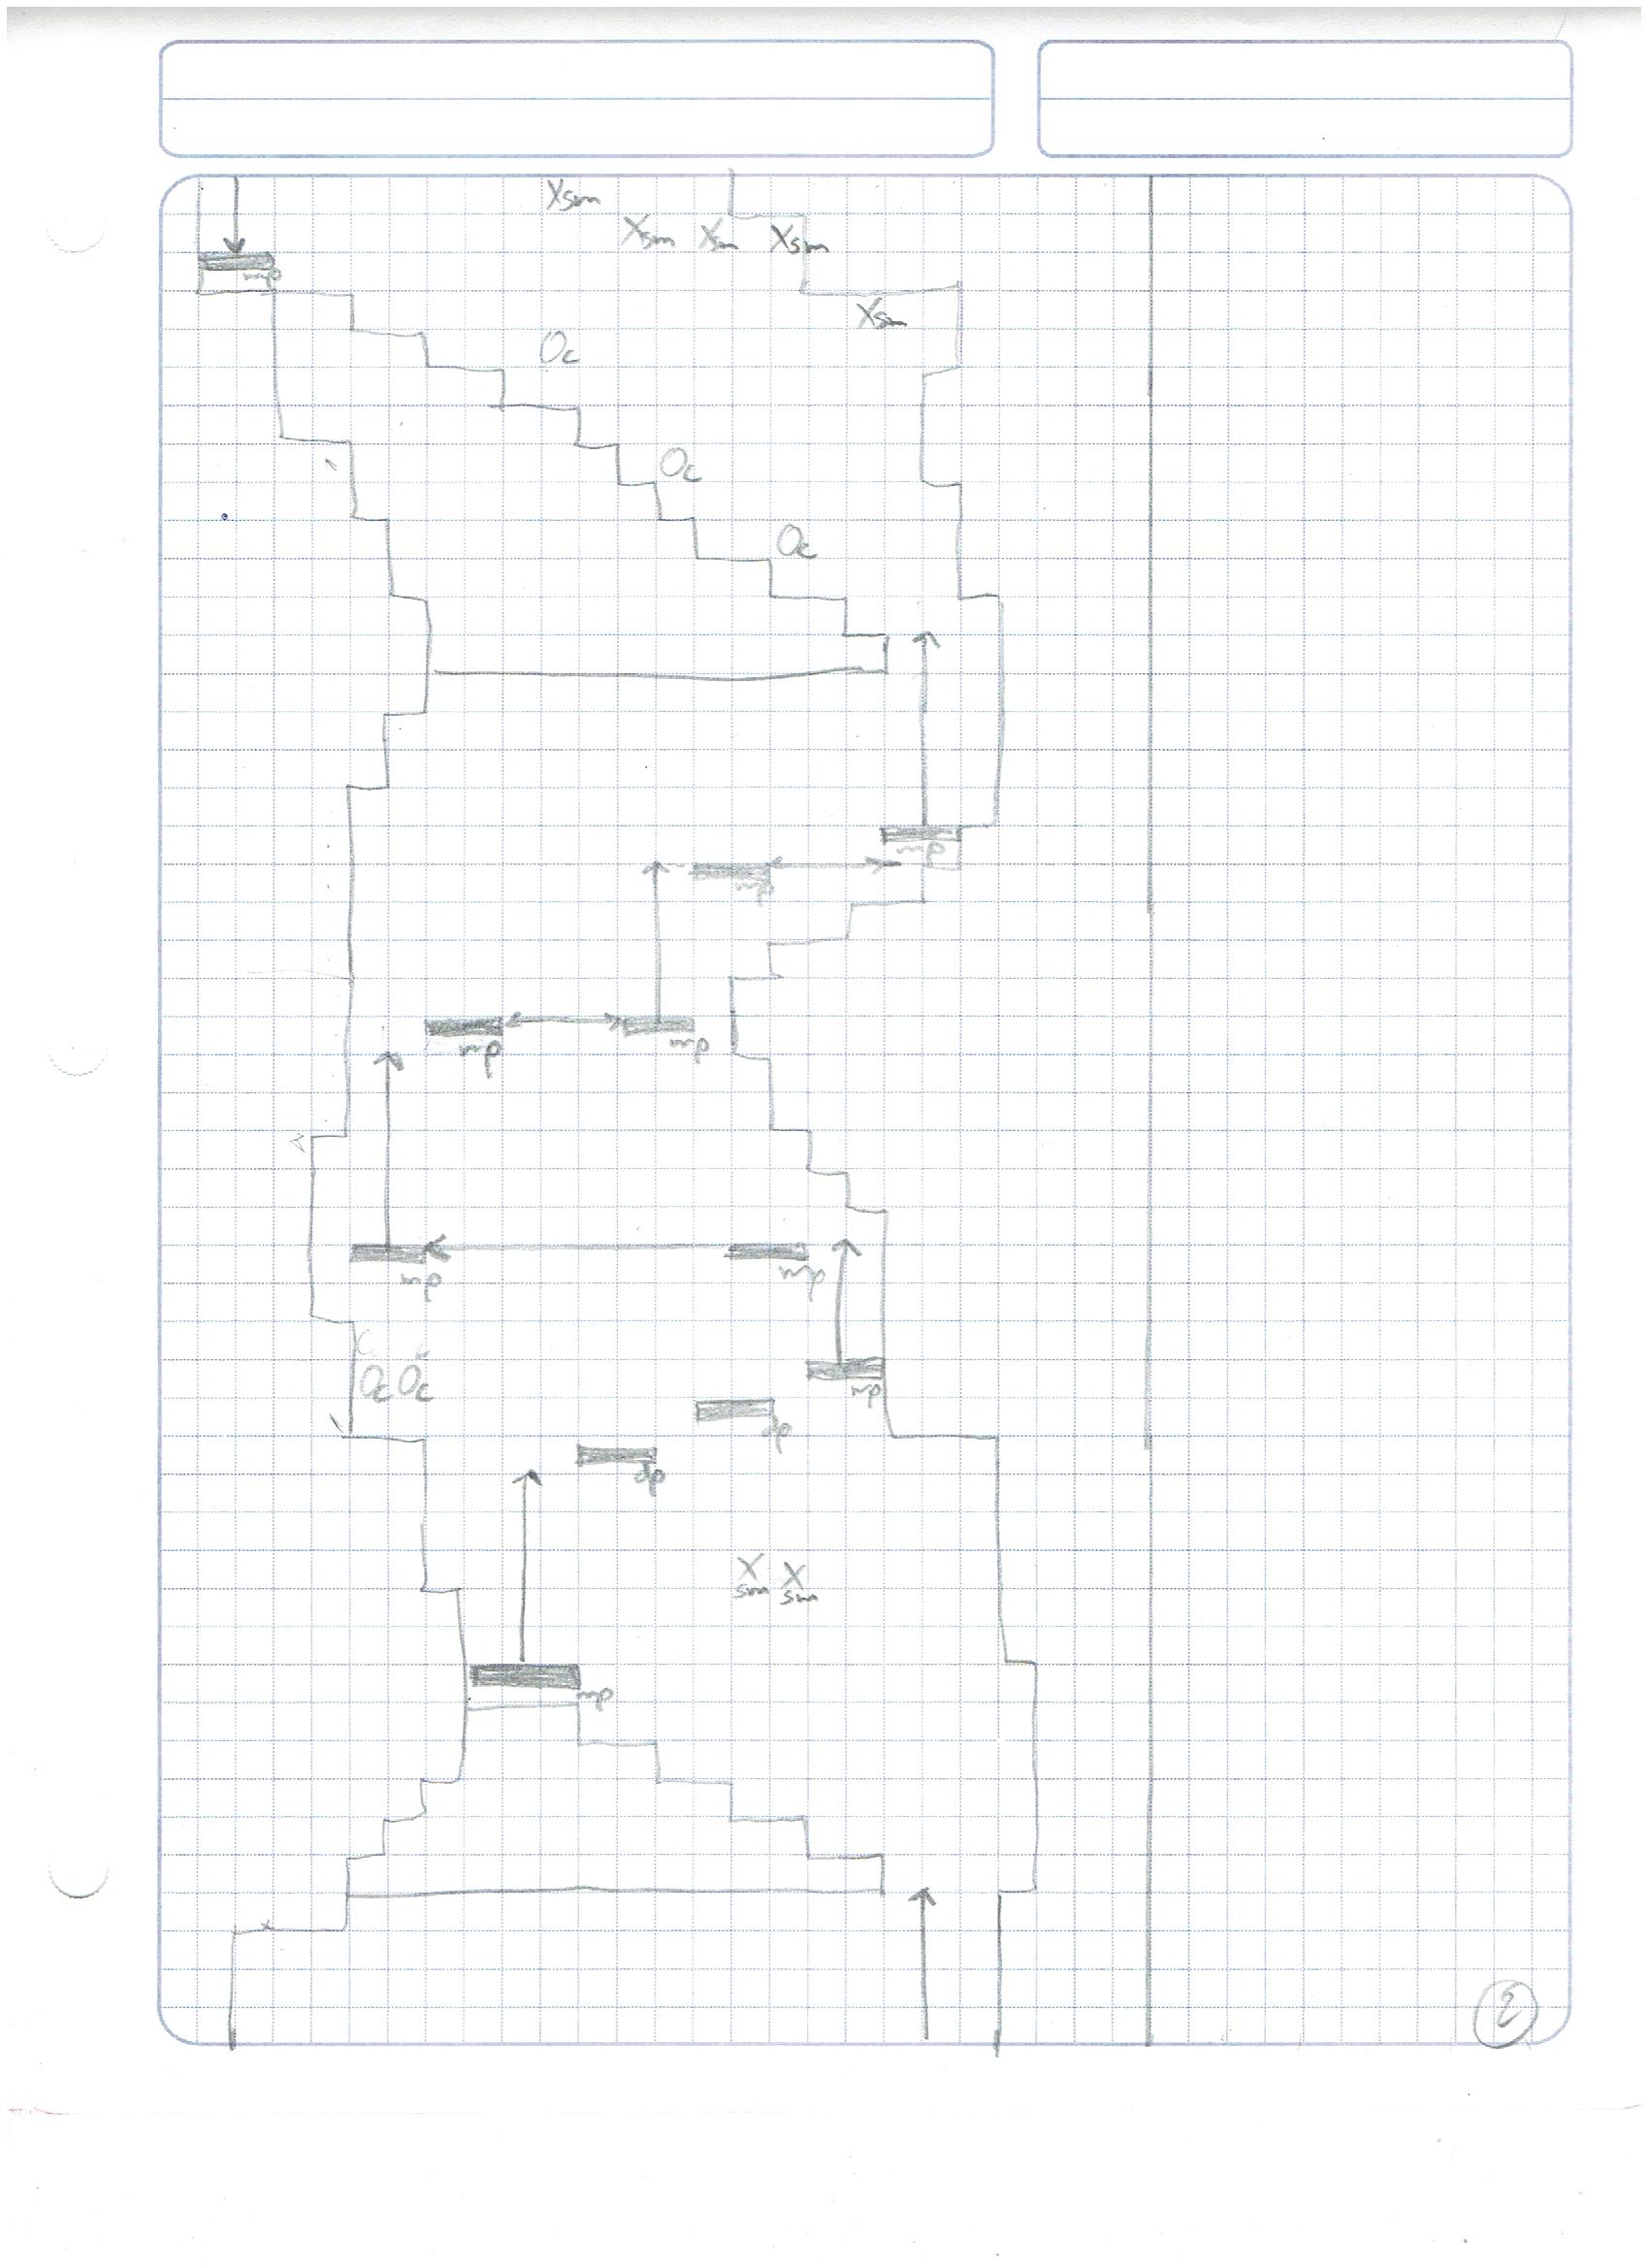
\includegraphics[width=5cm]{03TrabajoRealizado/DocProduccionR/imagenes/n3/03.jpeg}}
	\subfigure[Cuarta parte del nivel]{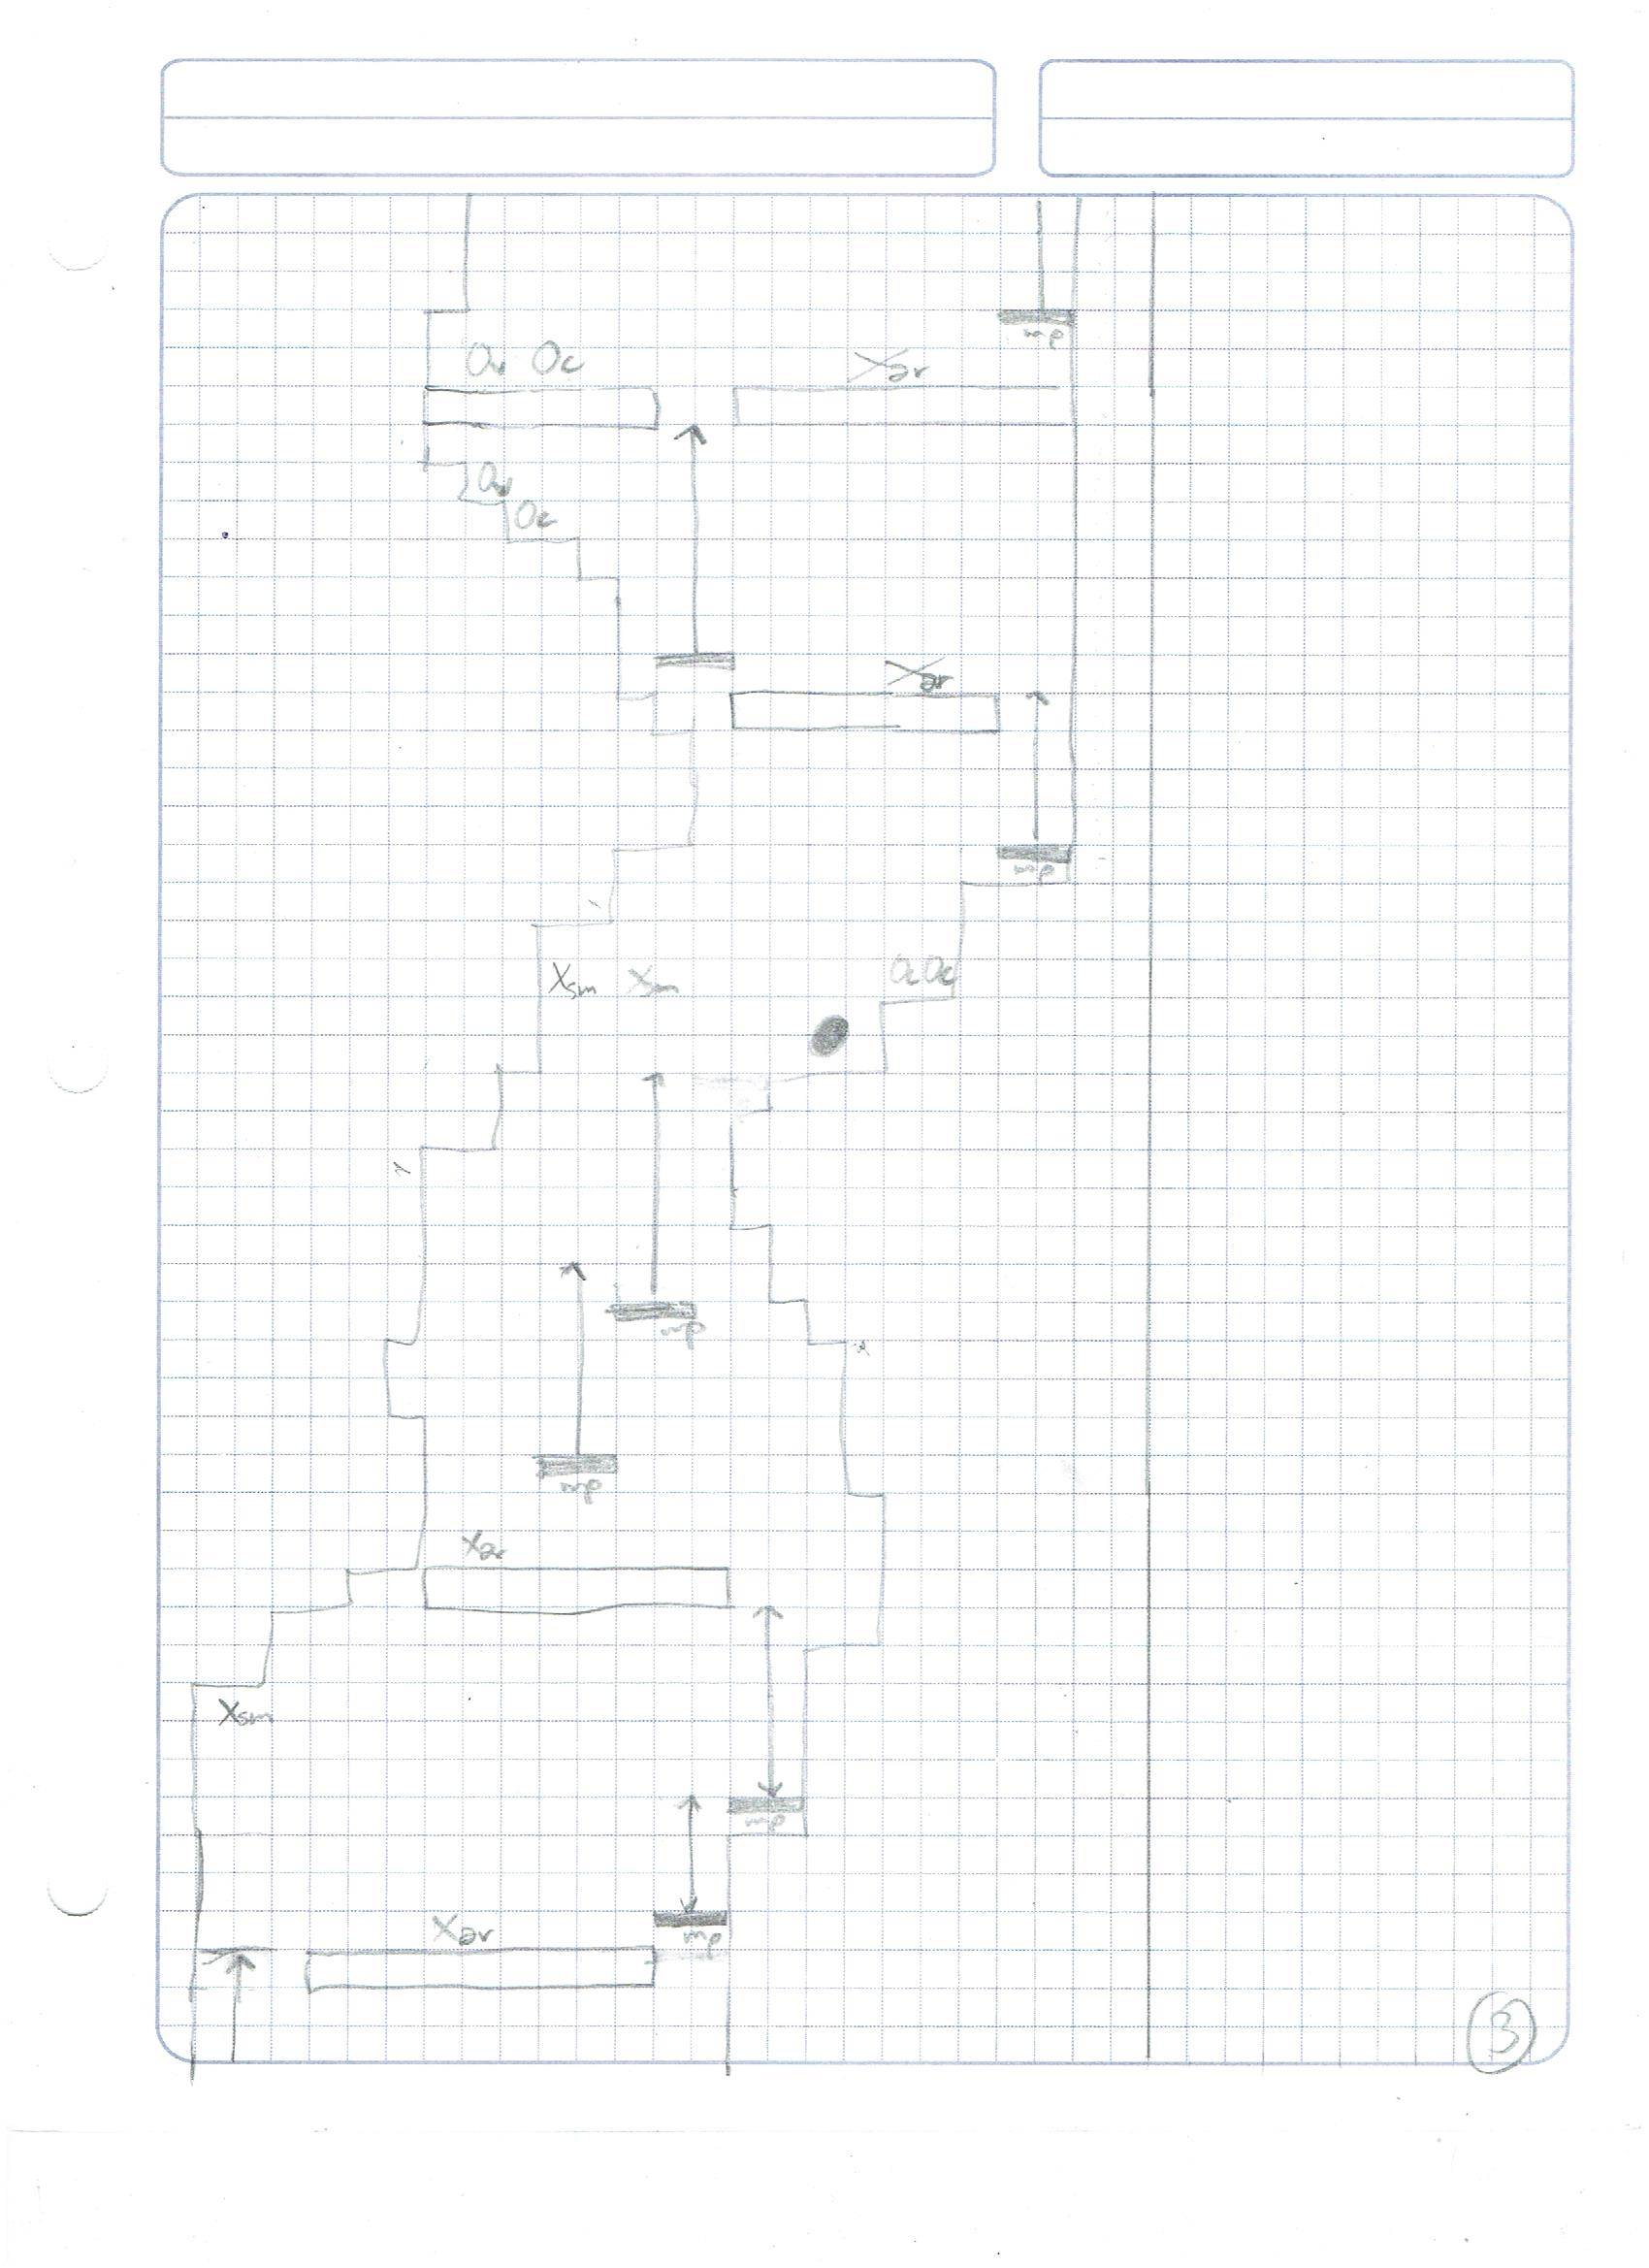
\includegraphics[width=5cm]{03TrabajoRealizado/DocProduccionR/imagenes/n3/04.jpg}}
	\caption{Maquetado de nivel tres} \label{fig:n01}
\end{figure}  

Después se lleva la tarea de tomar todos los componentes solo de manera visual y adecuar el tamaño necesario, tomando en cuenta las medidas de los componentes anteriores. Dichas imágenes se pueden ver en la \ref{fig:n02}.
\begin{figure}[htbp]
	\centering
	\subfigure[Imagen de cacao para recuperar vida]{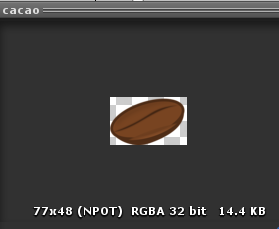
\includegraphics[width=5cm]{03TrabajoRealizado/DocProduccionR/imagenes/n3/n302.png}}
	\subfigure[Imagen de enemigo fantasma rojo]{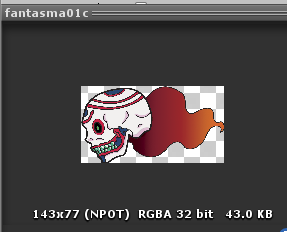
\includegraphics[width=5cm]{03TrabajoRealizado/DocProduccionR/imagenes/n3/n303.png}}
	\subfigure[Imagen de rugido de jefe enemigo]{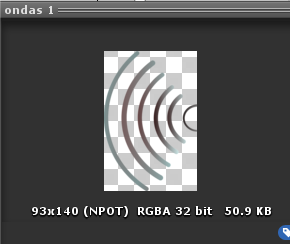
\includegraphics[width=5cm]{03TrabajoRealizado/DocProduccionR/imagenes/n3/n304.png}}
	\subfigure[Imagen de roca utilizada para daño]{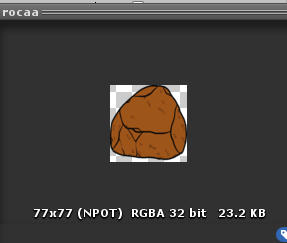
\includegraphics[width=5cm]{03TrabajoRealizado/DocProduccionR/imagenes/n3/n305.png}}
	\subfigure[Imagen de jefe enemigo jaguar Tepeyóllotl]{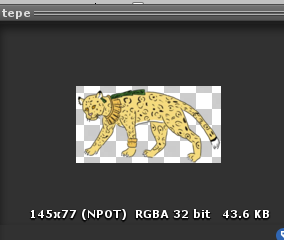
\includegraphics[width=5cm]{03TrabajoRealizado/DocProduccionR/imagenes/n3/n306.png}}
	\subfigure[Imagen de indicador de cambio de escena]{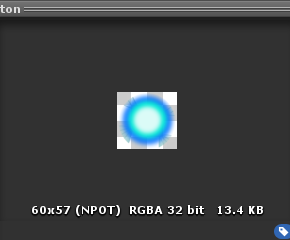
\includegraphics[width=5cm]{03TrabajoRealizado/DocProduccionR/imagenes/n3/n307.png}}
	\subfigure[Imagen de cara de jefe enemigo jaguar como indicador]{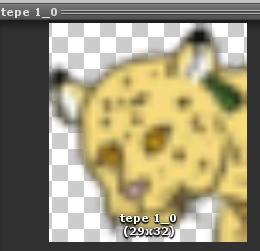
\includegraphics[width=5cm]{03TrabajoRealizado/DocProduccionR/imagenes/n3/n308.png}}
	\subfigure[Imagen de flor de vainilla para recuperar tonalli]{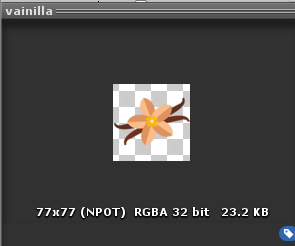
\includegraphics[width=5cm]{03TrabajoRealizado/DocProduccionR/imagenes/n3/n309.png}}
	\subfigure[Imagen de enemigo armadillo]{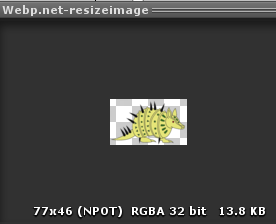
\includegraphics[width=5cm]{03TrabajoRealizado/DocProduccionR/imagenes/n3/n310.png}}
	\subfigure[Imagen de terreno rocoso]{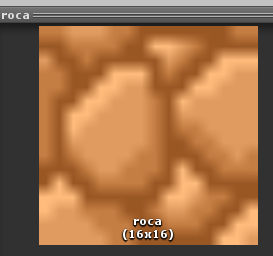
\includegraphics[width=5cm]{03TrabajoRealizado/DocProduccionR/imagenes/n3/n311.png}}
	\subfigure[Imagen de terreno con pasto]{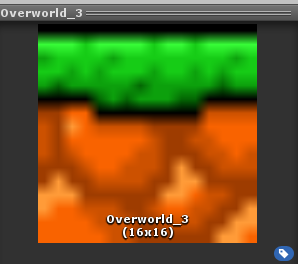
\includegraphics[width=5cm]{03TrabajoRealizado/DocProduccionR/imagenes/n3/n312.png}}
	\subfigure[Imagen de roca gigante]{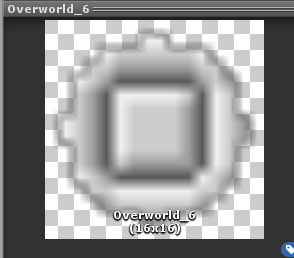
\includegraphics[width=5cm]{03TrabajoRealizado/DocProduccionR/imagenes/n3/n313.png}}
	\caption{Imágenes utilizadas para el nivel} \label{fig:n02}
\end{figure}

Después de reunir los componentes se da a la tarea de dar las acciones que realizarían descritas dentro de la figura \ref{fig:n03}. Se omite en esta parte los fantasmas enemigos que ya han sido realizados en niveles anteriores.
\begin{figure}[htbp]
	\centering
	\subfigure[Establecer que los picos tengan detección por debajo de ellos y despues caer para realizar daño.]{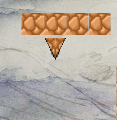
\includegraphics[width=5cm]{03TrabajoRealizado/DocProduccionR/imagenes/n3/lo0.png}}
	\subfigure[Establecer que la roca gigante detecte en una zona establecida el pase del jugador y después caiga rodando para estorbar el paso.]{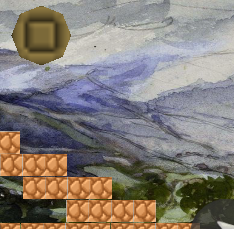
\includegraphics[width=5cm]{03TrabajoRealizado/DocProduccionR/imagenes/n3/lo1.png}}
	\subfigure[Ejemplo muestra de las plataformas que se mueven en dirección horizontal, la del lado izquierdo y vertical, la del lado derecho.]{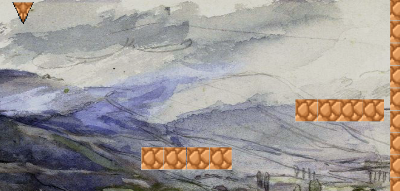
\includegraphics[width=5cm]{03TrabajoRealizado/DocProduccionR/imagenes/n3/lo2.png}}
	\subfigure[Piso que al tener contacto con el jugador este toma otra posición más abajo.]{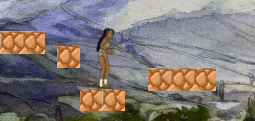
\includegraphics[width=5cm]{03TrabajoRealizado/DocProduccionR/imagenes/n3/lo3.png}}
	\subfigure[Ejemplo de como una vez que el jugador se quita de la posición sobre el piso, este vuelve a su lugar.]{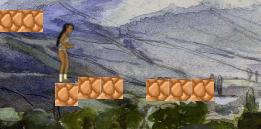
\includegraphics[width=5cm]{03TrabajoRealizado/DocProduccionR/imagenes/n3/lo4.png}}
	\caption{Muestra de comportamiento de objetos} \label{fig:n03}
\end{figure}

Ya que se tiene los objetos con los comportamientos deseados se procede a ubicarlos según correspondan como se ve en la \ref{fig:n04}.
\begin{figure}
	\centering
	\caption{Maquetado llevado al motor de juego Unity.}
	\label{fig:n04}
	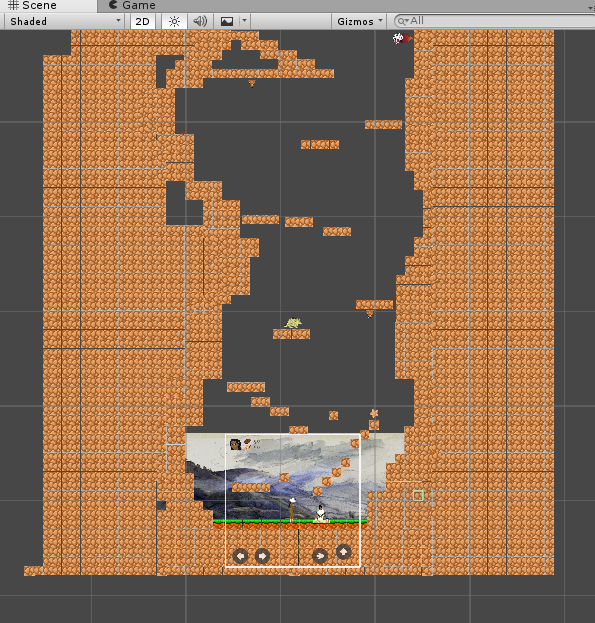
\includegraphics[width=0.5\textwidth]{03TrabajoRealizado/DocProduccionR/imagenes/n3/n301.png}
\end{figure}

Por último se establece las acciones que realiza el jefe enemigo Tepeyóllotl descritas en la siguiente figura \ref{fig:n05}.
\begin{figure}[htbp]
	\centering
	\subfigure[El enemigo se lanza en dirección al jugador con otro color.]{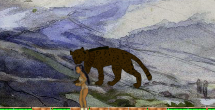
\includegraphics[width=5cm]{03TrabajoRealizado/DocProduccionR/imagenes/n3/n314.png}}
	\subfigure[El enemigo aparece rocas que van cayendo desde la parte superior.]{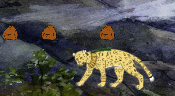
\includegraphics[width=5cm]{03TrabajoRealizado/DocProduccionR/imagenes/n3/n315.png}}
	\subfigure[El enemigo realiza un rugido.]{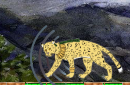
\includegraphics[width=5cm]{03TrabajoRealizado/DocProduccionR/imagenes/n3/n316.png}}
	\subfigure[El enemigo realiza un azote contra el piso apareciendo rocas a sus lados.]{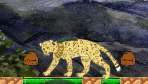
\includegraphics[width=5cm]{03TrabajoRealizado/DocProduccionR/imagenes/n3/n317.png}}
	\caption{Muestra de acciones de el jefe enemigo jaguar} \label{fig:n05}
\end{figure}

\section{Cuarto \textit{sprint} de producción}
Una vez definidas las nuevas estrategias de trabajo y que se atendieron 
las observaciones de los sinodales se procedió a realizar la maquetación de los 
niveles pares restantes y los \textit{sprites} faltantes. Al termino de este 
\textit{sprint} se obtienen más de 100 \textit{sprites} y las maquetas de los 
niveles pares.

\subsection{Creación de las maquetas de los niveles pares restantes}
Para la generación de las maquetas se sigue usando la plantilla creada durante 
la creación del primer demo del juego (ver figura \ref{fig:MaquetaPlantilla}). 
Para la creación de la maqueta también se crea un documento con todos los 
componentes de un nivel como son los enemigos, los ítems, los puntos de guardado, 
las plataformas y los obstáculos. Este documento se imprime y los objetos se 
recortan para ser pegados como estampas en las plantillas de diseño de las 
maquetas. En promedio la maqueta de cada nivel no excede de las 15 plantillas, 
sin embargo hay algunas que exceden este numero como la maqueta del cuarto nivel, 
la cual por su naturaleza de laberinto termino por ser más extensa que el 
resto. Por su parte los niveles correspondientes a los jefes de los niveles no 
sobrepasan de las tres plantillas, siendo la maqueta del jefe del sexto nivel 
la más pequeña de todas. 

%%
\begin{figure}[h]
	\centering
	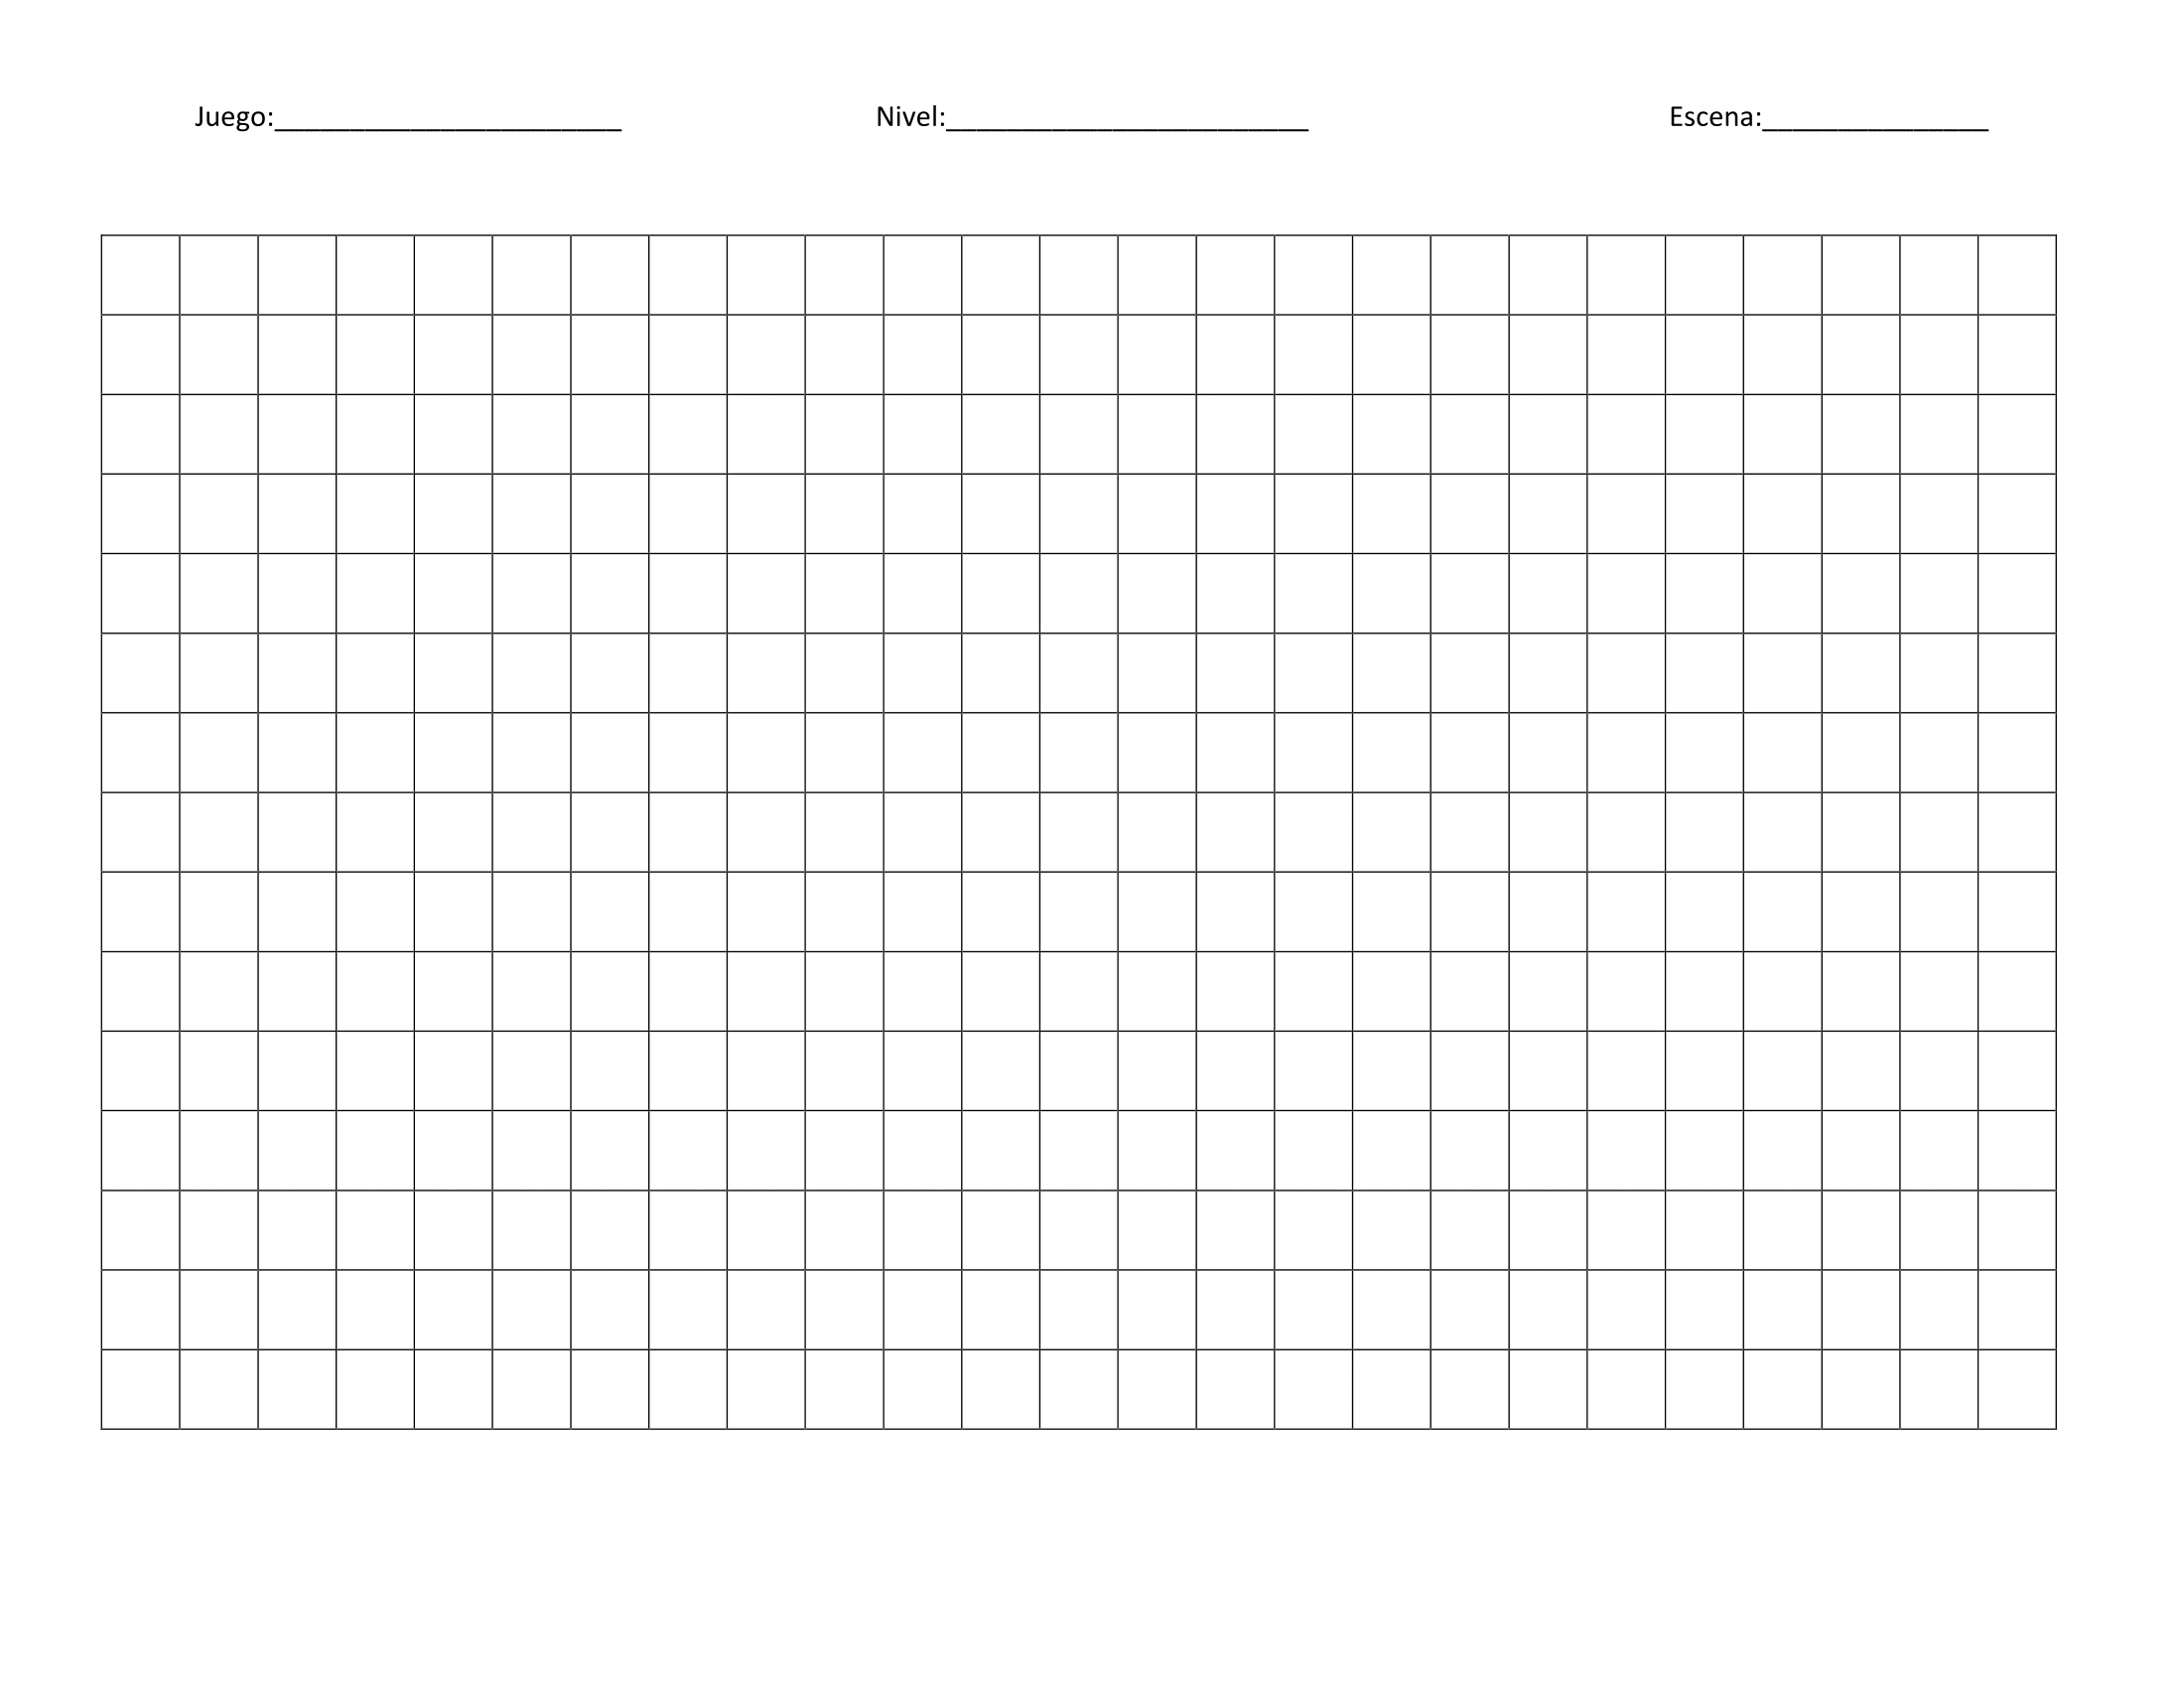
\includegraphics[width=0.6\textwidth]{03TrabajoRealizado/imagenes/maqueta-1.png}
 	\caption{Plantilla para la crecaión de niveles.}
	\label{fig:MaquetaPlantilla}		
\end{figure}

\subsection{Creación de los \textit{sprites} faltantes}
Lo siguiente a realizarse durante el cuarto \textit{sprint} fueron los \textit{sprites}, 
durante las modificaciones que se definieron en Trabajo Terminal 1 fue la 
utilización de un \textit{software} de animación en dos dimensiones para generar 
los \textit{sprites} restantes; sin embargo, el cambio de \textit{software} para 
generar los sprites fue descartado, esto debido a que se adquirió una nueva 
tableta digitalizadora que agilizó la creación de \textit{sprites}. Para Trabajo 
Terminal 2 se dibujaron y digitalizaron más de 100 \textit{sprites}. Para mejorar 
la experiencia visual del jugador se animaron \textit{sprites} que en los primeros 
demos eran estáticos como es el caso de los fantasmas del segundo nivel de la 
sección de plataformas (ver figura \ref{fig:FantasmaAnimacion}). 

%%
\begin{figure}[h]
	\centering
	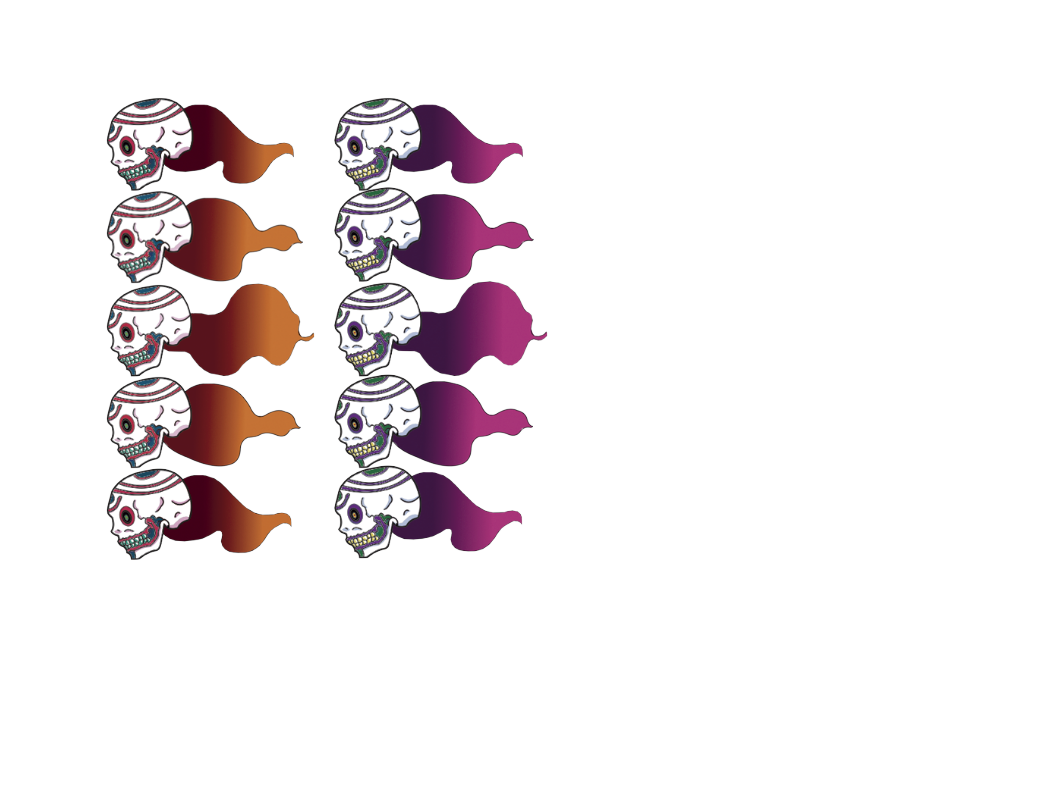
\includegraphics[width=0.6\textwidth]{03TrabajoRealizado/imagenes/fantasmas.png}
 	\caption{Bloques de animación para el enemigo de tipo fantasma.}
	\label{fig:FantasmaAnimacion}		
\end{figure}

Otros cambios en cuanto el aspecto visual del juego fue la integración de nuevos 
\textit{sprites} para el personaje jugable, los nuevos sprites incluyen la 
caracola que \textit{Malinalli} (ver figura \ref{fig:MalinalliCaracola}) emplea 
para atacar y que se obtiene al final del primer nivel de la sección de selva, 
estos \textit{sprites} para \textit{Malinalli} son utilizados únicamente en los 
niveles posteriores al primer nivel para darle sentido a la narrativa; para el 
segundo nivel se hizo algo parecido, los \textit{sprites} del personaje jugable 
fueron sustituidos por \textit{Malinalli} montando un ajolote (ver figura 
\ref{fig:MalinalliAjolote}), este cambio se hizo para que lo que el jugador vea 
dentro del nivel sea coherente con la narrativa propuesta y se mejore la inmersión del juego. 

\begin{figure}[h]
	\centering
	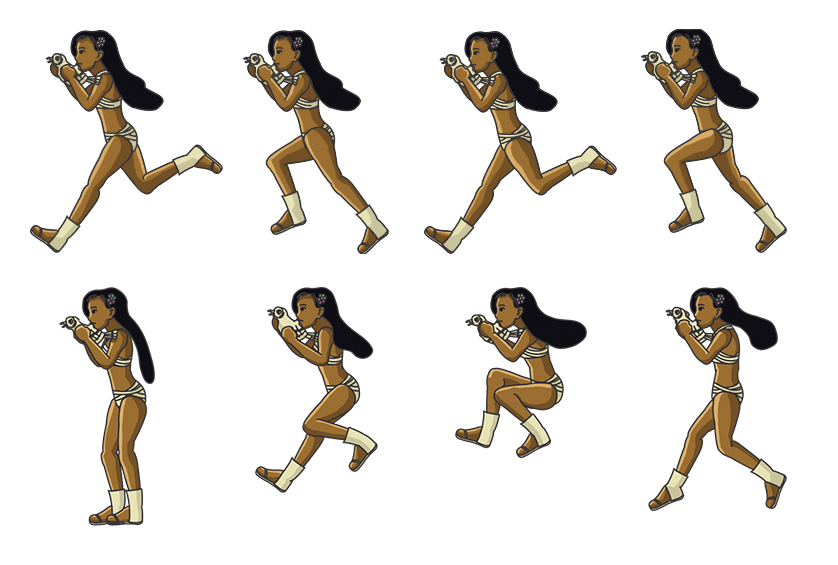
\includegraphics[width=0.4\textwidth]{03TrabajoRealizado/imagenes/MalinalliArma.png}
 	\caption{Bloques de animación para \textit{Malinalli} posterior a que ella obtiene la caracola.}
	\label{fig:MalinalliCaracola}		
\end{figure}

\begin{figure}[h]
	\centering
	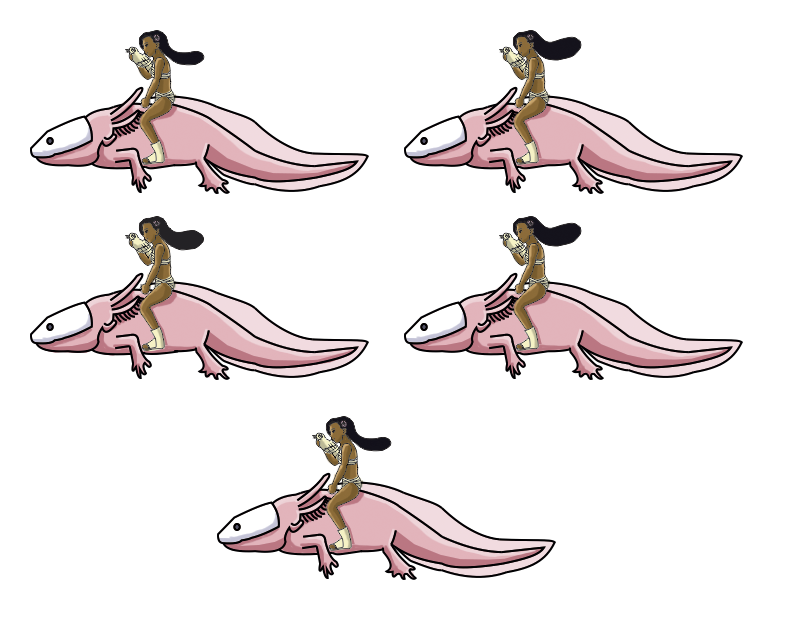
\includegraphics[width=0.5\textwidth]{03TrabajoRealizado/imagenes/MalinaliAjolote.png}
 	\caption{Bloques de animación para \textit{Malinalli} montando al ajolote del segundo nivel del juego.}
	\label{fig:MalinalliAjolote}		
\end{figure}

En lo que se refiere a los Jefes de cada nivel, no solo se crearon sus 
respectivos \textit{sprites}, también fue necesario la creación de los 
\textit{sprites} referentes a sus ataques, para el caso particular de 
\textit{Mictlantecuhtli} se dibujaron 30 \textit{sprites} tanto para la animación 
del personaje como para la animación de sus respectivos ataque (ver figura 
\ref{fig:Mictlantecutli}). Para el diseño de la interfaz gráfica de usuario
(\textit{GUI} por sus siglas en íngles) se emplearon \textit{sprites} de las 
paginas \textit{Kenney.nl} y \textit{Game Art 2D}. Es importante aclarar que la 
creación de \textit{sprites} pudo haber sido sustituida utilizando paquetes de 
\textit{sprites} que existen en la red y que son de licencia libre; sin embargo, 
con la creación de \textit{sprites} propios para el juego se consigue crearle una 
identidad visual propia al juego, esto permite que el jugador se identifique con 
mayor facilidad con el personaje y tenga una mejor asociación con el mundo y la 
historia que se le presenta dentro del juego [cita]. Si se desea ver a profundidad 
los {sprites} que se crearon se puede consultar el anexo \ref{Anexo:Personajes}. 


\begin{figure}[h]
	\centering
	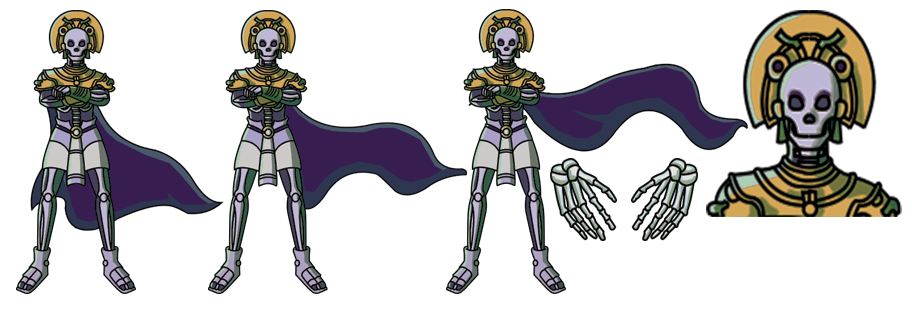
\includegraphics[width=0.6\textwidth]{03TrabajoRealizado/imagenes/Mictlantecuhtli.png}
 	\caption{Bloques de animación para \textit{Mictlantecuhtli}, jefe final del juego.}
	\label{fig:Mictlantecutli}		
\end{figure}

\subsection{Cierre del sprint}
Al terminar este \textit{sprint} se obtienen todas las maquetas de los niveles 
pares y los \textit{sprites} a utilizar de los mismos. Este \textit{sprint} se 
considera completado ya que se generaron todos los elementos que se tenían 
planeado. Como ultimo paso para este \textit{sprint}, se realiza el empaquetado 
de todos los \textit{sprites} creados durante el \textit{sprint}. 
\subsection{Detalles del proyecto}
Aquí se mostrará del proyecto el título, estudio, género, plataforma, fecha de inicio, fecha de término, lo planeado, en desarrollo, sin planear y terminado.
\\
\subsubsection{Título}
Yolotl

\subsubsection{Estudio}
ESCOM - IPN

\subsubsection{Plataforma}
Dispositivos móviles android

\subsubsection{Fecha de inicio}
26 febrero 2018
\subsubsection{Fecha de término}
1 Abril 2018
\subsubsection{Planeado}
El 48\%
\subsubsection{Desarrollo}
El 42\%
\subsubsection{Planear}
El 20\%
\subsubsection{Terminado}
El 32\%



\subsection{Sprint plan}
\subsubsection{SprintID}
05
\subsubsection{Inicio}
12 Marzo 2018
\subsubsection{Días}
7
\subsubsection{Fin}
18 Marzo 2018
\subsubsection{Meta}
Nivel 5
\subsubsection{Porcentaje}
El 16\% 


\subsection{Project chart}



\subsection{Feature log}

\subsubsection{FeatureID}
05
\subsubsection{Nombre}
N5
\subsubsection{Estado}
Planeado
\subsubsection{Días}
7
\subsubsection{SprintID}
05
\subsubsection{Comentarios}
-


\subsection{Sprint backlog}
\subsubsection{Sprint # backlog}
05
\subsubsection{Días}
7
\subsubsection{Tareas}
14
\subsubsection{Tendencia}
0
\subsubsection{Esfuerzo restante}
56
\subsubsection{Tendencia actual}
-
\subsubsection{Progreso ideal}
14
\subsubsection{Tareas restantes}
14
\subsubsection{Nombre de la tarea}
n5
\subsubsection{FeatureID}
05
\subsubsection{Miembro}
Rocío
\subsubsection{Rol}
Desarrollo
\subsubsection{Estado}
Planeado
\subsubsection{Esfuerzo}
14
\subsubsection{Números}



\subsection{Task chart - sprint "ggrafica"}



\subsection{Burn-down chart "grafica"}


\subsection{Task Slips}


\subsubsection{FeatureID}5
\subsubsection{Nombre}Maqueta
\subsubsection{Tarea}Realizar maqueta del nivel completo
\subsubsection{Miembro}Rocío
\subsubsection{Esfuerzo estimado}1
\subsubsection{Terminado}si
\subsubsection{Restante}0


\subsubsection{FeatureID} 5
\subsubsection{Nombre} Enemigos
\subsubsection{Tarea} Realizar el comportamiento de los enemigos o cualquier otra acción necesaria dentro del nivel
\subsubsection{Miembro} Rocio
\subsubsection{Esfuerzo estimado} 5
\subsubsection{Terminado} sí
\subsubsection{Restante} 0


\subsubsection{FeatureID} 5
\subsubsection{Nombre} Arte 1
\subsubsection{Tarea} Crear vista de los personajes
\subsubsection{Miembro} Rocío
\subsubsection{Esfuerzo estimado} 2
\subsubsection{Terminado} sí
\subsubsection{Restante} 0



\subsubsection{FeatureID} 5
\subsubsection{Nombre} Arte 2
\subsubsection{Tarea} Crear el diseño de los obstáculos
\subsubsection{Miembro} Rocío
\subsubsection{Esfuerzo estimado} 2
\subsubsection{Terminado} sí
\subsubsection{Restante} 0


\subsubsection{FeatureID} 5
\subsubsection{Nombre} Arte 3
\subsubsection{Tarea} Crear el diseño de los items
\subsubsection{Miembro} Rocio
\subsubsection{Esfuerzo estimado} 2
\subsubsection{Terminado} sí
\subsubsection{Restante} 0

\subsubsection{FeatureID} 5
\subsubsection{Nombre} Boss 1
\subsubsection{Tarea} Diseñar la máquina de estados del enemigo principal del nivel
\subsubsection{Miembro} Rocio
\subsubsection{Esfuerzo estimado} 2
\subsubsection{Terminado} sí
\subsubsection{Restante} 0

\subsubsection{FeatureID} 5
\subsubsection{Nombre} Boss 2
\subsubsection{Tarea} Crear la máquina de estados del enemigo principal del nivel
\subsubsection{Miembro} Rocio
\subsubsection{Esfuerzo estimado} 2
\subsubsection{Terminado} sí
\subsubsection{Restante} 0

\section{Sexto \textit{sprint} de producción}
En este \textit{sprint} se tiene como objetivo la implementación de todos los
actores del juego tanto a nivel de código como en la creación de los
\textit{GameObjects} para generar su posterior \textit{Assets}. En esta sección
no se hablan de aquellos actores que se hayan implementado desde Trabajo terminal
1 a no ser que su funcionalidad se haya rediseñado.

\subsection{Implementando los enemigos normales del juego}
Las primeras clases actoras en ser programadas fueron las correspondientes a los
enemigos normales, estas clases se programaron a la par que la clase \textit{Player}.
Si bien la clase \textit{Player} ya estaba programada desde los primeros prototipos,
esta clase no contaba con toda su funcionalidad implementada y la funcionalidad
faltante tuvo que ser implementada a la par que otras clases para verificar el
correcto funcionamiento en la interacción de clases como la de los enemigos y los
\textit{ítems}.
\\
\par
Al igual que con la clase \textit{Player},  existían enemigos desde los primeros prototipos; no obstante,
su funcionalidad tuvo que volver a ser implementada a fin de ofrecer un desempeño que
optimice recursos y agregue nuevas funcionalidades. A continuación, se listan los
cambios que presentan los enemigos de séptimo \textit{sprint} en relación de los
enemigos del primer prototipo:

    \begin{itemize}
         \item \textbf{Áreas de acción}: En el primer prototipo los enemigos ejecutaban
         sus patrones de movimiento y ataque sin importar que éstos se encontraran
         visibles para el jugador o no. Los enemigos del sexto \textit{sprint}
         cuentan con áreas de acción definida, lo que hace que sus patrones de
         movimientos y ataques solo se ejecuten si el jugador entra a estas áreas
         activas. Esto permite que el dispositivo no gaste recursos en objetos que no se
         encuentran visibles para el jugador (ver figura ).
        
             \begin{figure}[h]
                    \centering
                    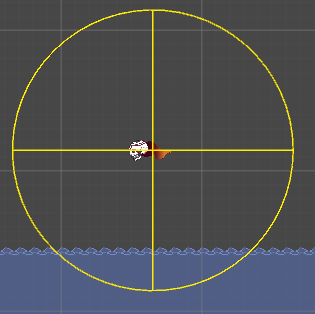
\includegraphics[width=0.4\textwidth]{03TrabajoRealizado/imagenes/EnemyRaycasting.png}
                    \caption{Ejemplo del área de acción del enemigo \textit{RedGhost}}
                    \label{fig:EnemyArea}
                \end{figure}
           
         \item \textbf{Cantidad de vida}: En el primer prototipo todos los enemigos
         eran derrotados por un único disparo, esto limitaba el factor de reto del
         juego al no ofrecer enemigos más resistentes al ataque del jugador. En el
         fin de ofrecer una nueva capa de complejidad a los enemigos se agrega a la
         clase \textit{Enemy} el atributo \textit{maxHealth} y \textit{healthAmount},
         estos atributos son los encargados de almacenar la máxima cantidad de vida
         que un enemigo puede tener y la vida actual de dicho enemigo (ver figura
         \ref{fig:EnemyAtributes}). La cantidad de
         vida sólo se actualiza cuando el enemigo es atacado por el jugador o cuando
         se reinicia el nivel. Para la actualización de la vida del enemigo se utiliza
         el comando \textit{Clamp} de la clase \textit{Math}, este comando permite
         especificar rangos con valores máximos y mínimos del resultado de operaciones,
         esto con la finalidad de que la vida actual del enemigo nunca sea cero y nunca
         sobrepase a su máximo de vida (ver figura \ref{fig:EnemyHealth}).
        
             \begin{figure}[h]
                    \centering
                    \includegraphics[width=0.6\textwidth]{03TrabajoRealizado/imagenes/EnemyClass.png}
                    \caption{Nuevos atributos para la clase \textit{Enemy}.}
                    \label{fig:EnemyAtributes}
            \end{figure}
            
            \begin{figure}[h]
                    \centering
                    \includegraphics[width=0.6\textwidth]{03TrabajoRealizado/imagenes/EnemyClassMethodHealth.png}
                    \caption{Actualización de la cantidad de vida de la clase
                    \textit{Enemy}.}
                    \label{fig:EnemyHealth}
            \end{figure}
            
         \item \textbf{Cantidad de daño}: Al igual que con la cantidad de vida, los
         enemigos del primer prototipo infringen la misma cantidad de daño sin
         importar su tipo; por lo que para tener enemigos más y menos fuertes se agrega
         el atributo \textit{damageAmount}. Un enemigo puede infringir daño al jugador
         cada vez que toca al jugador o cuando dispara un ataque. Cada vez que un
         enemigo o un disparo enemigo choca con el jugador, el objeto enemigo manda
         a llamar el método \textit{SetHealth} del \textit{Player} y le envía como
         parámetro el valor de su atributo \textit{damageAmount}, seguido de un segundo 
         método
         de la clase \textit{Player} llamado \textit{EnemyNockBack}, este método es
         el encargado de la animación que indica que el jugador ha recibido daño (ver
         figura \ref{fig:PlayerGetsDamage}).
            
            \begin{figure}[h]
                \centering
                \includegraphics[width=0.4\textwidth]{03TrabajoRealizado/imagenes/EnemyRaycasting02.png}
                \caption{Ejecución de los métodos \textit{SetHealth} y \textit{EnemyNockBack} de la clase \textit{Player}, los cuales actualizan la cantidad de vida del jugador y muestran la animación de que el jugador ha recibido daño.}
                \label{fig:PlayerGetsDamage}
            \end{figure}
            
         \item \textbf{Girar horizontalmente}: En el primer prototipo el enemigo era
         incapaz de girar sus \textit{Sprite} y su ataque una vez que el jugador lo sobrepasaba como se ve en la figura \ref{fig:EnemyBack}. Utilizando la posición del enemigo y la posición del jugador dentro del área activa, el enemigo puede voltear su sprite y su ataque con base al valor de la distancia entre éste y el jugador:
         \begin{itemize}
             \item Si la posición del enemigo es mayor que las del jugador, el enemigo
             mantiene su orientación inicial.
             \item Si la posición del jugador es mayor que la del enemigo, el enemigo
             se voltea.
         \end{itemize}          

         Voltear un \textit{Sprite} no representa mayor problema en código; sin 
         embargo, el
         voltear un \textit{sprite} cuyo colisionador no es simétrico como el de 
         la figura
         \ref{fig:FixerCollider}. Esto puede representar un problema cuando se tiene
         que detectar colisiones, tal y como ocurre con los enemigos de tipo 
         \textit{RedGost} y
         \textit{PulpleGost}; para evitar alterar la detección de colisiones se 
         crea una nueva
         clase auxiliar llamada \textit{FixerCollider},  cuyo objetivo es ajustar 
         la posición
         del colisionador una vez que el personaje se gira como se puede observar en
         la figura \ref{fig:FixerCollider}.
        
         \begin{figure}[h]
                \centering
                \includegraphics[width=0.4\textwidth]{03TrabajoRealizado/imagenes/voltearEnemigo01.png}
                \caption{En los primeros prototipos el enemigo es incapaz de girar su sprite y su ataque una vez que el jugador se coloca tras de éste.}
                \label{fig:EnemyBack}
        \end{figure}
        
        \begin{figure}[h]
              \centering
               \subfigure[ Ejemplo de un colisionador no simétrico respecto al \textit{sprite}.] {\includegraphics[width=0.3 \textwidth]{03TrabajoRealizado/imagenes/voltearEnemigo02.png}}
       
             \subfigure[Al girar el sprite de manera horizontal la posición del colisionador no se modifica]{\includegraphics[width=0.3 \textwidth]{03TrabajoRealizado/imagenes/voltearEnemigo04.png}}
         
            \subfigure[Posición del colisionador modificada al emplear la clase \textit{FixerCollider}.] {\includegraphics[width=0.3 \textwidth]{03TrabajoRealizado/imagenes/voltearEnemigo03.png}}
            
              \caption{Comportamiento del colisionador antes y después de la implementación de la clase \textit{FixerCollider}.}
              \label{fig:FixerCollider}
        \end{figure}
        
         \item \textbf{Trigger Collider}: En el primer prototipo el colisionador del
         enemigo tenía una configuración del tipo sólido lo que ocasionaba que cuando
         el enemigo chocaba con otro enemigo o con algún ataque enemigo este se
         estancara o fuera empujado por el objeto contra el que chocaba.
         Para corregir este comportamiento se configura el colisionador como uno de tipo
         trigger (ver figura \ref{fig:EnemyColliderTri}).  
            
            \begin{figure}[h]
                \centering
                \includegraphics[width=0.3\textwidth]{03TrabajoRealizado/imagenes/Colisonador01.png}
                \caption{Configuración actual del colisionador de los enemigos.}
                \label{fig:EnemyColliderTri}
            \end{figure}    
        
         \item \textbf{Rigidbody2D}: Para evitar el comportamiento mencionado en el
         \textit{Trigger Collider} también fue necesario modificar la configuración
         del componente \textit{Rigidbody2D}, este componente pasa de estar en modo
         \textit{Dynamic} a modo \textit{Kinematic} lo que permite evitar que el objeto
         de juego reaccione conforme a las leyes físicas comunes.   
             
             \begin{figure}[h]
                \centering
                \includegraphics[width=0.3\textwidth]{03TrabajoRealizado/imagenes/Colisonador02.png}
                \caption{Configuración actual del componente \textit{Rigidbody2D} de
                los enemigos.}
                \label{fig:EnemyRigidBody}
            \end{figure}
    \end{itemize}

Para implementar cada uno de los patrones de movimiento de los enemigos es necesario
utilizar posiciones auxiliares que indiquen el límite del movimiento del personaje,
salvo en la clase Vulture ya que este explota al hacer contacto con el jugador. En la figura \ref{fig:JaguarCode} se puede observar el patrón de movimiento del enemigo de tipo jaguar expresado en código. Este comportamiento consiste en un movimiento recto horizontal de un punto A a un punto B y de regreso, haciendo una pausa en el movimiento cada vez que el jaguar ha alcanzado cualquiera de los puntos A o B (ver figura ).
\\
\par
            \begin{figure}[h]
                \centering
                \includegraphics[width=0.3\textwidth]{03TrabajoRealizado/imagenes/PatronJaguar.png}
                \caption{Patrón de movimiento del enemigo tipo Jaguar expresado en
                código.}
                \label{fig:JaguarCode}
            \end{figure}
            
            \begin{figure}[h]
                \centering
                \includegraphics[width=0.3\textwidth]{03TrabajoRealizado/imagenes/saltoFelino.jpg}
                \caption{Patrón de movimiento del enemigo tipo Jaguar expresado en
                su comportamiento visual.}
                \label{fig:JaguarBeha}
            \end{figure}


Para resaltar la muerte de un enemigo se agrega un efecto especial de explosión
acompañado de un efecto de sonido para la explosión del personaje. Para esta
funcionalidad se implementa la clase \textit{SFXCtrl} y \textit{AudioCtrl} para 
manejar los efectos
de especiales y el sonido respectivamente, siendo estos los primeros controladores
en ser implementados.

\subsection{Implementando los enemigos jefes del juego}
Para la implementación de los enemigos jefes se reutilizan las configuraciones de los enemigos
normales referentes a las componentes \textit{Rigidbody2D} y \textit{Colisionador}, así como 
a la clase \textit{Enemy} para el manejo de vida y el uso de los efectos
de sonido y de explosiones para la muerte del jefe.
\\
\par
La lógica teórica tras los jefes del juego está inspirada por el jefe
\textit{Roxas} (ver figura \ref{fig:Roxas}) del juego \textit{Kingdom Hearts 2
Final Mix}. Dentro de \textit{Kingdom Hearts 2 Final Mix}, \textit{Roxas} es uno
de los jefes que requiere mayor habilidad de juego para ser derrotado, ya que a
diferencia del resto de los jefes de \textit{Kingdom Hearts 2 Final Mix}, el
patrón de ataque de \textit{Roxas} es totalmente aleatorio. Es decir, el jugador
puede saber en qué consiste cada uno de los ataques de este jefe, pero desconoce
el orden en el que estos serán ejecutados, salvo por algunos ataques que están
condicionados a una secuencia de ataque anterior.  Con los jefes del juego
\textit{Yolotl} sucede algo parecido, el jugador puede llegar a conocer lo tipos
de ataque que posee un jefe determinado pero la secuencia de ejecución de los
ataques está programada para que sea aleatoria, lo que puede generar experiencias
de juego muy sencillas o bastante retadoras para el jugador. El anterior
comportamiento se logra simulando una máquina de estados[referencia] 
con un arreglo de tipo booleano llamado \textit{whatCanDo}, en el cual solo un índice puede tener el
valor verdadero cada vez que se actualiza el estado y dependiendo del valor del
índice del valor verdadero será el ataque que ejecutará el enemigo. Después de
cada ataque el enemigo espera un tiempo determinado antes de asignar el siguiente
y ejecutarlo. Para ayudar al lector a comprender el funcionamiento de los jefes se
explica nuevamente usando como ejemplo al jefe \textit{Itzpapálotl} del nivel
cuatro. El jefe \textit{Iztpapálotl} cuenta con cuatro acciones:
    \begin{itemize}
        \item \textbf{\textit{WaitForAction:}} Espera un tiempo determinado y asigna
        un nuevo índice valor verdadero del arreglo de valores booleanos. Se activa
        si \textit{whatCanDo}[0] es verdadero.
        \item \textbf{\textit{shotFire}}: Dispara cuatro esferas de fuego que siguen
        al jugador y en caso de no chocar con este después de un tiempo se destruyen.
        Se activa si \textit{whatCanDo}[1] es verdadero.
        \item \textbf{\textit{useShell}}: Invoca un círculo de fuego que protege a
        \textit{Itzpapálotl} de cualquier daño, el escudo de fuego también puede
        infringir daño al jugador si hace contacto con éste. Se activa si
        \textit{whatCanDo}[2] es verdadero.
        \item \textbf{\textit{CreateButterflies}}: Invoca mariposas en tres puntos
        del campo, las mariposas también infringen daño al jugador y desaparecen
        después de un tiempo. Se activa si \textit{whatCanDo}[3] es verdadero.
    \end{itemize}
Al inicializarse el jefe \textit{Itzpapálotl whatCanDo}[0] es igual a cero. Por
lo que \textit{Itzpapálotl} ejecuta \textit{waitForAction}, al terminar la
ejecución de \textit{waitForAction}, \textit{whatCanDo}[0] es igual a falso y un nuevo
índice tiene ahora el valor verdadero. Supóngase ahora \textit{whatCanDo}[2] es
verdadero. \textit{Itzpapálotl} ejecuta \textit{useShell}, al terminar su
ejecución asigna \textit{whatCanDo}[2] como falso y asigna a \textit{whatCanDo}[0]
como verdadero. Nuevamente \textit{Itzpapálotl} espera unos segundos y actualiza
\textit{whatCanDo}. Por la naturaleza aleatoria de la actualización,
\textit{whatCanDo}[2] puede ser nuevamente verdadero o lo puede ser cualquier
otro índice exceptuando al 0 o a un número mayor que el índice máximo del
arreglo. En la figura se muestra la verificación de los valores de
\textit{whatCanDo} antes de la ejecución de cualquiera de los ataques que
tienen asignados. En la figura \ref{fig:EnemyMaquina} se muestra un ejemplo en
código de la maquina de estados del jefe \textit{Itzpapálotl}.
\\
\par
Por la forma en la que fue diseñado el comportamiento de la máquina de estados,
el nivel de dificultad que presente el jefe está dado en función de dos variables:
\textit{damageAmount} y \textit{timeBetweenAttacks}, correspondientes a la
cantidad de daño que el jefe puede infringir en el jugador y al tiempo que se
espera para actualizar los valores de \textit{waitForAction}. A mayor cantidad
de daño y menor tiempo de espera entre ataques, mayor será la dificultad para
derrotar al enemigo.

            \begin{figure}[h]
                \centering
                \includegraphics[width=0.5\textwidth]{03TrabajoRealizado/imagenes/RoxasBoss.jpg}
                \caption{\textit{Roxas} es el jefe más retador de \textit{Kingdom Hearts 2 Final Mix}. $ [Imagen] (2014)$ Recuperado de: \url{https://images.khinsider.com/2014\%20Uploads/05/Screenshots\%205-30/KHII_battle_03_EN\%20copy_1401446206.jpg}}
                \label{fig:Roxas}
            \end{figure}04R

            \begin{figure}[h]
                \centering
                \includegraphics[width=0.5\textwidth]{03TrabajoRealizado/imagenes/ActualMaquinaJefe.png}
                \caption{Ejemplo de la máquina de estados del enemigo jefe.}
                \label{fig:EnemyMaquina}
            \end{figure}

\subsection{Implementando los ataques enemigos del juego}
Dentro del juego existen seis tipos de ataques enemigos:
    \begin{itemize}
        \item \textbf{Disparos con una trayectoria definida:} Este tipo de
        disparo sigue una trayectoria recta horizontal como se ve en la figura         
        \ref{fig:Enemyshot}.
        Para evitar la saturación de objetos dentro del juego, todos los disparos de
        este tipo se destruyen después de un tiempo. Para implementar este tipo de
        ataque se crea un \textit{GameObject} y se le agregan los siguientes
        componentes:
            \begin{itemize}
                \item \textbf{Collisionador:} El colisionador permite detectar si este
                ataque hace contacto con el \textit{Player} o con el suelo del nivel,
                en el primer caso se infringe daño al \textit{Player} y se destruye el
                \textit{GameObject}, en el segundo el \textit{GameObject} solo se
                destruye.
                \item \textbf{\textit{Rigidbody2D}}: El \textit{rigidbody2D} se
                configura
                con la opción \textit{kinematic} para evitar que el movimiento del
                disparo se vea afectado por la gravedad. Este componente permite en el
                código agregarle una velocidad al objeto.
                \item \textbf{\textit{DestryWithDelay}}: Componente creado por medio de
                la clase del mismo nombre, esta clase destruye al \textit{GameObject}
                que la contiene después de una cantidad determinada de tiempo.
                \item \textbf{\textit{EnemyBullet}}: Esta clase controla en la velocidad
                y dirección del movimiento del disparo, también tiene como atributo el
                daño que causa la bala y gestiona las colisiones del objeto.
            \end{itemize}
        Este tipo de disparo es empleado por los enemigos de tipo \textit{RedGost,
        Tepeyóllotl} y por \textit{Mictlantecuhtli}.
            
            \begin{figure}[h]
                \centering
                \includegraphics[width=0.5\textwidth]{03TrabajoRealizado/imagenes/disparoTrayectoria.png}
                \caption{Ejemplo de un disparo de una trayectoria definida.}
                \label{fig:Enemyshot}
            \end{figure}
            
        \item \textbf{Disparos que siguen al jugador}: Este tipo de disparo sigue un
        comportamiento y configuración parecida al anterior con la diferencia que en
        este tipo el disparo seguirá al jugador hasta impactarse contra éste o
        destruirse después de un tiempo si no colisiona contra el jugador. Este
        comportamiento requiere que el disparo tenga una referencia a la posición del
        jugador para moverse hacia él, en la figura \ref{fig:FollowedShot}se puede ver
        la implementación de disco comportamiento en código. Este ataque es utilizado
        por los enemigos de tipo \textit{Mictlantecuhtli}, \textit{Tepeyóllotl},
        \textit{Itzpapálotl, Xochitonal} y \textit{Tlazolteolt}. Para todos estos
        enemigos el disparo tiene el mismo efecto que es el de infringir
        daño en el jugador; sin embargo, en el tipo de \textit{Tlazolteolt} este tipo de
        disparo también puede disminuir la cantidad de \textit{Tonalli} del Player.
            
            \begin{figure}[h]
                \centering
                \includegraphics[width=0.5\textwidth]{03TrabajoRealizado/imagenes/disparoSigue.png}
                \caption{Implementación en código del comportamiento del disparo que sigue al jugador.}
                \label{fig:FollowedShot}
            \end{figure}        
        
        \item \textbf{Escudo de defensa que desaparece después de un tiempo}: Este
        ataque es efectuado por \textit{Itzpapálotl}. Al invocarse este escudo el
        enemigo no se ve afectado por los ataques del jugador. Este escudo no puede ser
        destruido y desaparece después de un tiempo que se invocó; este comportamiento
        se logra utilizando el método \textit{Invoke}, este método permite ejecutar
        métodos después de una cantidad de segundos; por lo que la desactivación se
        consigue mandando a llamar al método responsable de esto con \textit{Invoke}
        y asignando una cantidad determinada de segundos de espera.
        Inflige daño al jugador al hacer contacto con él.

        \item \textbf{Escudo de defensa que debe de ser destruido para desaparecer}:
        Ataque utilizado por \textit{Tlazolteolt}. Este escudo puede ser destruido
        por disparos del jugador y no desaparece al cabo de un tiempo. Al igual que el
        anterior protege al enemigo de los ataques del jugador e inflige daño si el
        jugador hace contacto con éste. Este tipo de escudo no cuenta con un método
        que lo desactive, en su lugar tiene una cantidad de vida determinada y que
        al llegar a cero, por efecto de los ataques del jugador, desaparece y reaparece
        hasta que el enemigo jefe lo vuelva a convocar.

        \item \textbf{Objetos que aparecen en posiciones cuya aparición tiene un tiempo
        de duración}: Este ataque es empleado por \textit{Itzpapálotl} y
        \textit{Mictlantecuhtli}. Cuando se activa provoca que se creen instancias del
        \textit{GameObject} que contiene la clase \textit{Butterfly}. Esta clase genera
        un movimiento vertical ascendente e inflige daño al jugador al hacer contacto
        con esta. La creación de estos \textit{GameObjects} se mantiene activa por un
        periodo de tiempo y después desactiva.Este funcionamiento se logra de una
        manera similar al comportamiento del escudo de defensa que desaparece después
        de un tiempo utilizando el método \textit{Invoke}. En la figura se puede
        observar la implementación en código de este tipo de ataque.  

        \item \textbf{Objetos que aparecen en posiciones de manera periódica}: Este
        ataque genera una lluvia de huesos o de piedras que le infringen daño al
        jugador una vez hacen contacto con este de lo contrario se destruyen al hacer
        contacto con el suelo. Para la creación de los objetos se utiliza el método
        \textit{Invoke} el cual controla la cantidad de \textit{GameObject} que se
        crean. Este ataque es utilizado por \textit{Mictlantecuhtli} y
        \textit{Tepeyóllotl}.
    \end{itemize}
 
\subsection{Implementando los obstáculos}
Una de las características de un juego de plataformas es la existencia de diferentes
obstáculos que el jugador debe de superar por medio de saltos\cite{Ref_JuegoDisenio}.
En \textit{Yolotl} se diseñaron e implementaron diferentes tipos de obstáculos
para ofrecer una variedad de retos al jugador, a continuación, se describe cada
uno de ellos y cómo fue que fueron implementados en el juego:
    \begin{itemize}
        \item \textbf{Plataforma que se mueve:} Es uno de los elementos más comunes de
        los juegos de plataforma, este   obstáculo consiste en una superficie de que
        se mueve de una posición a otra, ver figura \ref{fig:MovingPlatform}. dentro
        del juego se creó la clase \textit{MovingPlatform} para este tipo de obstáculo.
        \textit{MovingPlatform} tiene por atributos las posiciones a las que se moverá,
        velocidad a la que se moverá. Para su movimiento la clase hace uso de cuatro
        vectores de posiciones \textit{pos01, pos02, startPos} y \textit{nextPos}.
        \textit{Pos01} y \textit{pos02} son las posiciones límite que alcanzará la
        plataforma, \textit{startPos} es la posición hacia la que la plataforma inicie
        su movimiento inicial y \textit{nextPos} es la siguiente posición a la que se
        ira la plataforma una vez que haya alcanzado un límite. Manejar el
        comportamiento de las plataformas móviles con este sistema de posiciones
        permite que la plataforma pueda tener movimiento horizontal, vertical o diagonal
        sin la necesidad de reescribir código. Al igual que con los enemigos las
        plataformas de este tipo tienen un radio de área activa para evitar que su
        comportamiento se ejecute si no están visibles al jugador. Asignar el movimiento
        de la plataforma no es suficiente para su correcto funcionamiento, ya que
        cuando el movimiento de la plataforma es horizontal, ésta se desplaza sin el
        personaje ya que por sí misma no es capaz de asignarle un movimiento al jugador,
        por tal motivo fue necesario crear una nueva etiqueta para las plataformas
        llamada \textit{Platform} y asignar dos nuevos parámetros en las colisiones
        al jugador
        una para cuando entra en contacto con el colisionador de la plataforma y otra
        cuando sale. Cuando el jugador entra en contacto con el colisionador de la
        plataforma se le asigna un parentesco con la posición de la plataforma, lo
        que le permite seguir el movimiento de la plataforma, este parentesco se
        rompe cuando el jugador sale de la plataforma, en la figura
        \ref{fig:MovingPlatformCol} se puede ver esto en código. Adicionalmente,
        se utilizó el comando \textit{OnDrawGizmos} para dibujar la trayectoria de la
        plataforma a fin de facilitar la configuración de las plataformas móviles en la
        construcción de los niveles, ver figura \ref{fig:MovingPlatformWay}.
            
            \begin{figure}[h]
                \centering
                \includegraphics[width=0.5\textwidth]{03TrabajoRealizado/imagenes/plataformaMovil.jpg}
                \caption{Comportamiento de la plataforma que se mueve de manera visual.}
                \label{fig:MovingPlatform}
            \end{figure}
            
            \begin{figure}[h]
                \centering
                \includegraphics[width=0.5\textwidth]{03TrabajoRealizado/imagenes/plataformaColisiones.png}
                \caption{Gestión de la respuesta ante diferentes colisiones para
                garantizar el comportamiento de una plataforma que se mueve de manera
                horizontal.}
                \label{fig:MovingPlatformCol}
            \end{figure}
            
            \begin{figure}[h]
                \centering
                \includegraphics[width=0.5\textwidth]{03TrabajoRealizado/imagenes/plataformaConfig.png}
                \caption{Uso del método \textit{OnDrawGizmos} para visualizar la
                trayectoria de una plataforma que se mueve.}
                \label{fig:MovingPlatformWay}
            \end{figure}

        \item \textbf{Plataforma que cae}: Este tipo de plataforma se cae después de
        que el jugador se posiciona sobre ella. Para evitar que la plataforma caiga
        instantáneamente una vez que el jugador ha caído sobre ella, un tiempo de
        retraso se le asigna a la caída.

        \item \textbf{Plataforma con más de dos posiciones de control}: esta plataforma
        puede seguir patrones complejos movimiento como círculos, rectángulos o
        cuadrados. Su funcionamiento es similar a la plataforma que se mueve con la
        diferencia de que soporta más de dos posiciones de control; para esto se vale
        de un arreglo de posiciones en donde el atributo de \textit{nextPos} recorre
        todo el arreglo de posiciones y al llegar al último elemento del arreglo se
        le asigna el valor del primer elemento reiniciando el recorrido, ver figura .

        \item \textbf{Viento}: Ese obstáculo crea una corriente de viento que empuja
        al jugador hacia el vacío, ver figura . Para crear este obstáculo se crean
        tres clases: \textit{PushingObstacle}, \textit{WindCreator} y
        \textit{WindHelper}. La primera controla el movimiento del viento a crear.
        La segunda crea el viento por periodos de tiempo dejando un tiempo de
        inactividad para que el jugador pueda pasar y la tercera activa al creador
        de viento cuando el jugador entra en el área activa del obstáculo, cada clase
        está instanciada en un \textit{GameObject} diferente. En un principio solo
        existían las clases \textit{PushingObstacle} y \textit{WindCreator}, lo que
        provoca que el creador de viento cree viento aun cuando el obstáculo no es
        visible para el jugador; esto ocasiona la creación de muchos
        \textit{GameObjects} innecesarios para el viento, por tal motivo se crea la
        clase \textit{WindHelper} para controlar la activación del
        creador de viento.  Para definir los periodos de creación de viento y de pausa
        de viento es necesario probar diferentes valores para asignar los tiempos de
        creación y de pausa del viento. Luego de varias pruebas se definen los
        siguientes tres valores: 4 para el tiempo activo de creación, 8 para el tiempo
        de pausa de viento y 0.4 para la pausa entre creación de instancias de viento.

        \item \textbf{Estalagmitas}: Este obstáculo se cae e inflige daño en el
        jugador cuando éste pasa por debajo del obstáculo, ver figura .  Para
        implementar este obstáculo se crean dos clases: \textit{Stalagmite} y
        \textit{StalagmiteCtrl}. La primera clase gestiona la caída del objeto y el
        daño que le infringe al jugador si choca con este o la destrucción del objeto
        en caso de que choque con el suelo. La segunda clase se encarga de indicarle
        a la clase \textit{Stalagmite} que el jugador va a pasar bajo de ella para que
        inicie su caída. En la figura \ref{fig:StalagmiteConf} se puede ver la
        configuración de ambos objetos dentro de un nivel.
        
            \begin{figure}[h]
                \centering
                \includegraphics[width=0.3\textwidth]{03TrabajoRealizado/imagenes/StalagmiteConfig.png}
                \caption{Configuración de los diferentes \textit{GameObjects} que
                conforman el obstáculo estalagmita.}
                \label{fig:StalagmiteConf}
            \end{figure}
        
        \item \textbf{Obstáculo que hace daño}: este obstáculo infringe daño al jugador
        cuando éste hace contacto con él y no puede ser destruido por el mismo. Este
        tipo de obstáculo se puede encontrar en el segundo nivel en la etapa de
        plataforma. Para su implementación se crea la clase \textit{DamageObstacle} y 
        esta
        gestiona el daño que infringe el obstáculo pudiendo generar obstáculos que
        causen más o menos daños que otros.

        \item \textbf{Xólotl en su forma Colibrí}: Este obstáculo tiene un
        comportamiento parecido a la plataforma con más de dos posiciones de
        control anteriormente descrita, con la diferencia de que su movimiento
        describe una línea y no un circuito cerrado; por otro lado, al morir el
        jugador este obstáculo regresa a su posición inicial. Este obstáculo aparece
        únicamente en el nivel 6, donde el jugador deberá cruzar distintos segmentos
        del mapa sobre este obstáculo y tendrá que vencer a los enemigos que vayan
        apareciendo para avanzar, ver figura .
    \end{itemize}

\subsection{Implementando los ítems y los objetos coleccionables}
Las últimas clases actoras en ser implementadas fueron los ítems, los objetos
coleccionables y los puntos de guardado, ya que en el caso de los ítems y los
puntos de guardado se necesitaba que el jugador sufriera daño, gastara
\textit{tonalli} o muriera ya fuera a causa de enemigos u obstáculos.
\\
\par
Dentro del juego existen dos tipos de ítems: Los que recuperan cantidad de vida y
los que recuperan cantidad de tonalli. Ambos tienen un funcionamiento similar: como
atributos sus respectivas clases tienen una cantidad de lo que van a restaurar
(sea \textit{tonalli} o vitalidad), al hacer contacto con el jugador le incrementan
dicho atributo en la cantidad que tienen asignada y se destruyen mostrando un
efecto de brillos y un efecto de sonido.
\\
\par
En lo que se refiere a los objetos coleccionables dentro del juego se crea la
clase CollectableObjects, clase encargada de destruir los objetos coleccionables
una vez que el jugador los ha tocado, dejando la tarea de actualizar el marcador
al jugador. Para poder lograr la actualización del atributo \textit{score} del
\textit{Player} se asignaron etiquetas para los objetos coleccionables y dependiendo
de dichas etiquetas se gestiona la actualización de los marcadores, esto debido a que
la función de los objetos coleccionables depende directamente del nivel en el que
se encuentre el jugador; por ejemplo, para los perros que aparecen en el segundo
nivel, hacer contacto con uno de ellos no solo actualiza el marcador sino también
incrementa el poder que tendrá el Jefe de este nivel, por lo tanto
la actualización visual del marcador deberá incluir cuantos perros se han tocado
y en cuanto se ha incrementado el poder del jefe(ver figura
\ref{fig:CollectableObjects}); mientras que en el nivel 4, los coleccionables
son llaves y su función es la de desbloquear la transición al siguiente nivel
solo si se han juntado todas las llaves; visualmente esta actualización solo
requiere de la actualización de un elemento en pantalla (ver figura 
\ref{fig:CollectableObjects}). Para solucionar esto se crearon dos etiquetas 
para cada tipo de coleccionable: \textit{CollectableDog} y 
\textit{CollectableKey}.  Dejando al gestor de colisiones de la clase 
\textit{Player} verificar por medio de la etiqueta de qué tipo de coleccionable 
se trata e invoca al controlador de la interfaz gráfica de los marcadores del 
juego o \textit{HUB}.
            
            \begin{figure}[h]
              \centering
               \subfigure[El marcador referente a los perros se encuentra en cero, ya
               que el jugador no ha tocado ninguno de estos.] {\includegraphics[width=0.3 \textwidth]{03TrabajoRealizado/imagenes/InterfazJuego06.png}}
       
             \subfigure[Al tocar un perro el marcador referente al conteo de ellos se actualiza junto al del poder del jefe.]{\includegraphics[width=0.3 \textwidth]{03TrabajoRealizado/imagenes/InterfazJuego07.png}}
            
              \caption{Interacción entre el jugador y los objetos coleccionables del nivel.}
              \label{fig:CollectableObjects}
        \end{figure}

\subsection{Implementación de los puntos de guardado}
Los puntos de guardado o \textit{checkpoints} son los actores encargados de
hacer aparecer al jugador en una posición del nivel una vez que éste haya muerto,
evitando que el jugador pierda su progreso dentro del nivel. Un
\textit{checkpoint} se activa cuando el jugador hace contacto con éste. La
funcionalidad de este actor está dada por la clase \textit{CheckPoint}, esta clase
tiene como atributos(ver figura \ref{fig:CheckAtri}):

\begin{itemize}
    \item \textit{\textbf{isActive}}: Atributo booleano. Cuando es verdadero indica
    que el jugador  ha pasado por el checkpoint. Solo puede haber un único checkpoint
    activo.
    \item \textit{\textbf{CheckPointsList}}: Arreglo de GameObjects que instancian
    la clase CheckPoint.
\end{itemize}

Cuando el jugador entra en contacto con el \textit{checkPoint}, éste manda a
llamar el método \textit{ActivateCheckPoint}, este método toma todos los
elementos que hay en  \textit{CheckPointsList} y vuelve su atributo
\textit{isActive} falso, después vuelve verdadero el atributo \textit{isActive}
del \textit{checkPoint} que fue tocado por el jugador. Cuando el jugador muere
se manda a llamar el  método \textit{GetActivePosition}, este método busca el
\textit{checkPoint} activo y revive al jugador en esa posición. En la figura
\ref{fig:CheckMethod} se muestran los métodos de esta clase.

Existen dos tipos de \textit{checkPoints}:
    \begin{itemize}
        \item \textbf{\textit{CheckPoint} vacío}: este \textit{checkPoint} no 
        tiene ningún
        \textit{sprite} asignado y se encuentra al inicio del nivel. Está activo 
        por defecto
        y si el jugador muere sin antes tocar algún otro \textit{checkPoint}, la
        posición de este \textit{checkPoint} es donde aparecerá al revivir.
        \item \textbf{\textit{CheckPoint} normal}: Este \textit{checkPoint} tiene un
        búho como \textit{sprite} y una animación para cuando el jugador interactúa con
        él.
    \end{itemize}
    
\begin{figure}[h]
                \centering
                \includegraphics[width=0.3\textwidth]{03TrabajoRealizado/imagenes/checkpoint.png}
                \caption{Atributos de la clase \textit{CheckPoint}}
                \label{fig:CheckAtri}    
\end{figure}

\begin{figure}[h]
                \centering
                \includegraphics[width=0.3\textwidth]{03TrabajoRealizado/imagenes/checkpointmethods.png}
                \caption{Métodos de la clase \textit{CheckPoint}}
                \label{fig:CheckMethod}    
\end{figure}

\subsection{Cierre del sprint}
Al término de este \textit{sprint} se cuenta con todos los \textit{Assets} de
los actores organizados en diferentes carpetas como \textit{Player, Obstacles, Enemies},
etc. Este \textit{sprint} se cierra con éxito y deja todos los elementos listos
para la construcción de las clases controladoras.


\subsection{Sprint plan 7}
\subsubsection{SprintID}
07
\subsubsection{Inicio}
29 Enero 2018
\subsubsection{Fin}
18 Febrero 2018
\subsubsection{Meta}
Nivel 7
\subsubsection{Porcentaje}
El 16\% 


\subsubsection{FeatureID}
07
\subsubsection{Nombre}
N7
\subsubsection{Estado}
Planeado
\subsubsection{SprintID}
07
\subsubsection{Comentarios}
-


\subsection{Sprint backlog 7}
\subsubsection{Sprint # backlog}
07
\subsubsection{Tareas}
14
\subsubsection{Tendencia}
0
\subsubsection{Esfuerzo restante}
56
\subsubsection{Tendencia actual}
-
\subsubsection{Progreso ideal}
14
\subsubsection{Tareas restantes}
14
\subsubsection{Nombre de la tarea}
n7
\subsubsection{FeatureID}
07
\subsubsection{Miembro}
Rocío
\subsubsection{Rol}
Desarrollo
\subsubsection{Estado}
Planeado
\subsubsection{Esfuerzo}
14



\subsection{Task Slips 9}


\subsubsection{FeatureID}7
\subsubsection{Nombre}Maqueta
\subsubsection{Tarea}Realizar maqueta del nivel completo
\subsubsection{Miembro}Rocío
\subsubsection{Esfuerzo estimado}1
\subsubsection{Terminado}si
\subsubsection{Restante}0


\subsubsection{FeatureID} 7
\subsubsection{Nombre} Enemigos
\subsubsection{Tarea} Realizar el comportamiento de los enemigos o cualquier otra acción necesaria dentro del nivel
\subsubsection{Miembro} Rocio
\subsubsection{Esfuerzo estimado} 5
\subsubsection{Terminado} sí
\subsubsection{Restante} 0


\subsubsection{FeatureID} 7
\subsubsection{Nombre} Arte 1
\subsubsection{Tarea} Crear vista de los personajes
\subsubsection{Miembro} Rocío
\subsubsection{Esfuerzo estimado} 2
\subsubsection{Terminado} sí
\subsubsection{Restante} 0



\subsubsection{FeatureID} 7
\subsubsection{Nombre} Arte 2
\subsubsection{Tarea} Crear el diseño de los obstáculos
\subsubsection{Miembro} Rocío
\subsubsection{Esfuerzo estimado} 2
\subsubsection{Terminado} sí
\subsubsection{Restante} 0


\subsubsection{FeatureID} 7
\subsubsection{Nombre} Arte 3
\subsubsection{Tarea} Crear el diseño de los items
\subsubsection{Miembro} Rocio
\subsubsection{Esfuerzo estimado} 2
\subsubsection{Terminado} sí
\subsubsection{Restante} 0

\subsubsection{FeatureID} 7
\subsubsection{Nombre} Boss 1
\subsubsection{Tarea} Diseñar la máquina de estados del enemigo principal del nivel
\subsubsection{Miembro} Rocio
\subsubsection{Esfuerzo estimado} 2
\subsubsection{Terminado} sí
\subsubsection{Restante} 0

\subsubsection{FeatureID} 7
\subsubsection{Nombre} Boss 2
\subsubsection{Tarea} Crear la máquina de estados del enemigo principal del nivel
\subsubsection{Miembro} Rocio
\subsubsection{Esfuerzo estimado} 2
\subsubsection{Terminado} sí
\subsubsection{Restante} 0

\subsection{Octavo \textit{sprint} de producción}
En este \textit{sprint} se implementa en código la funcionalidad de todos los 
elementos controladores del juego y sus auxiliares, exceptuando a los 
controladores de los niveles ya que éstos se desarrollarán en el décimo 
\textit{sprint} dado que se requieren los niveles terminados para comprobar su 
funcionalidad.

\subsubsection{Controlador de Audio}
Este controlador es el encargado de gestionar los efectos de sonido del 
juego. Logra su funcionamiento con ayuda de la clase controladora 
\textit{AudioCtrl} y de la clase auxiliar \textit{PlayerAudio}. 
\\
\par
La clase \textit{PlayerAudio} está compuesta de los atributos del tipo 
\textit{AudioClip}. Por convención los archivos de audio que \textit{Unity} 
soporta pueden ser del tipo \textit{MP3}, \textit{OGG}, \textit{WAV}, entre 
otros, en relación a tamaño del archivo y calidad de audio se opta por utilizar 
los archivos de tipo \textit{OGG}. Para la importación de los archivos de audio 
se elige la configuración que se muestra en la figura \ref{fig:AudioClipConfi}, 
ya que ésta se disminuye el tiempo de carga de los audios y el espacio en 
memoria de almacenamiento que utilizan dentro de la aplicación. 
\textit{PlayerAudio} contiene cinco pistas de audio correspondientes a los 
efectos de sonido cuando: 
	\begin{itemize}
		\item El jugador hace contacto con un objeto coleccionable, como una 
		llave o un \textit{xoloitzcuintle}.
		\item El jugador hace contacto con un ítem.
		\item El jugador dispara \textit{tonalli}.
		\item Un enemigo es destruido.
		\item El jugador muere.
	\end{itemize}	 

\textit{PlayerAudio} se vale de la serialización para su funcionamiento(ver 
figura \ref{fig:PlayerAudio}), esta clase funge como un organizador de elementos 
para su visualización en el \textit{GameInspector}, como se ve en la figura 
\ref{fig:PlayerAudioConf}.   

	\begin{figure}[h]
		\centering
		\includegraphics[height=0.15 \textheight]{03TrabajoRealizado/imagenes/playerAudioConfig.png}
		\caption{Configuración de la importación de los archivos de audio.}
		\label{fig:AudioClipConfi}
	\end{figure}

	\begin{figure}[h]
		\centering
		\includegraphics[height=0.15 \textheight]{03TrabajoRealizado/imagenes/playerAudio.png}
		\caption{Serialización de la clase \textit{PlayerAudio}}
		\label{fig:PlayerAudio}
	\end{figure}


	\begin{figure}[h]
		\centering
		\includegraphics[height=0.1 \textheight]{03TrabajoRealizado/imagenes/audioCtrlGameInsp.png}
		\caption{Atributos organizados en el \textit{GameInspector} gracias a la serialización de la clase \textit{PlayerAudio}.}
		\label{fig:PlayerAudioConf}
	\end{figure}

Por su parte la clase \textit{AudioCtrl} tiene como atributos la clase 
\textit{PlayerAudio}, un vector de tres dimensiones para la posición del 
personaje que mande a llamar los métodos que invocan los audios y una instancia 
de la misma clase \textit{PlayerAudio} para la perseverancia de datos. Los 
métodos que contiene la clase son para invocar determinado audio, para esa 
funcionalidad se utiliza el método \textit{PlayClipAtPoint}, el cual necesita 
como atributos un objeto de tipo \textit{AudioClip} y un vector de tres 
dimensiones. Cada método que invoca un efecto de audio es mandado a llamar en la 
parte del código que implementa dicha funcionalidad, por ejemplo en el método 
\textit{SetHealth} del la clase \textit{Enemy} se agrega la linea de código que 
invoca el audio para la destrucción de un Enemigo en donde se maneja la muerte 
del enemigo. En la figura se pueden ver los atributos y los métodos de la clase 
\textit{AudioCtrl}.  

	\begin{figure}[h]
		\centering
		\includegraphics[height=0.3 \textheight]{03TrabajoRealizado/imagenes/audioCtrl.png}
		\caption{Atributos y métodos de la clase \textit{AudioCtrl}.}
		\label{fig:AudioCrl}
	\end{figure}

\subsubsection{Controlador de Diálogos}\label{ControladorDialogo}
Este controlador se emplea en la cinemáticas del juego.El controlador de 
Diálogos se vale de cuatro clases para su funcionamiento: 
\textit{Dialogue}, \textit{Dialogues}, \textit{DialogueFile} y 
\textit{DialogueCtrl}. 
\\
\par
Las clases \textit{Dialogue} y \textit{Dialogues}, son clases de tipo auxiliar. Ambas clases son serializadas y el objetivo de ellas es el de organizar la información en el \textit{GameInspector}. La clase \textit{Dialogue} tiene como atributos un \textit{string} para almacenar el nombre del personaje al que pertenece el dialogo y una lista de tipo \textit{string} para los diálogos. Por su parte la clase \textit{Dialogues} tiene como atributo una lista de tipo \textit{Dialogue}. El objetivo de la clase \textit{Dialogues} es la de almacenar todos los diálogos de la cinemática. En la figura \ref{fig:Dialogues} se puede ver la definición de las clases \textit{Dialogue} y \textit{Dialogues}.
\\
\par
La clase \textit{DialogueFile} se encarga de la gestión de los diálogos, al contenerlos y activar la visualización de los mismos por medio de la clase \textit{DialogueCtrl}. 
\\
\par 
La clase \textit{DialogueCtrl} se encarga de la visualización de los diálogos 
dentro de la escena. Por tal motivo parte de sus atributos son 
\textit{GameObjects} del tipo \textit{Text} de la \textit{UI}. La clase 
\textit{DialogueCtrl} visualiza los diálogos tomando el contenido de la clase 
\textit{Dialogue} y extrayendo elemento por elemento. De cada elemento extraído 
se obtiene su lista de diálogos y se almacena esta lista en un \textit{Queue} y 
se muestra en pantalla cada dialogo. La transición entre diálogos se hace si el 
jugador oprime el botón de salto, ver figura \ref{fig:NextDialogueBottom}. Una 
vez que el controlador ha mostrado todos los diálogos de un elemento. Los 
diálogos se visualizan por medio de una animación que nuestra carácter por 
carácter, en la figura \ref{fig:DialoguesCtrl} se muestra el método encargado de 
mostrar esta animación.   

	\begin{figure}[h]
		\centering
		\includegraphics[height=0.3 \textheight]{03TrabajoRealizado/imagenes/dialogueFile.png}
		\caption{Serialización de las clases \textit{Dialogue} y \textit{Dialogues}.}
		\label{fig:Dialogues}
	\end{figure}

	\begin{figure}[h]
		\centering
		\includegraphics[height=0.2 \textheight]{03TrabajoRealizado/imagenes/DialogueOnScreen.png}
		\caption{La transición entre diálogos se hace si el jugador oprime el 
		botón de salto, este botón es el que se encuentra encerrado en rojo.}
		\label{fig:NextDialogueBottom}
	\end{figure}

	\begin{figure}[h]
		\centering
		\includegraphics[height=0.15 \textheight]{03TrabajoRealizado/imagenes/dialogueController02.png}
		\caption{El método \textit{TypeSentences} es el encargado de animar el texto de los diálogos al mostrarlos en pantalla}
		\label{fig:DialoguesCtrl}
	\end{figure}

\subsubsection{Controlador de los datos del juego}
El controlador de datos del juego es el encargado de gestionar los datos 
relacionados al progreso del jugador, es decir los niveles desbloqueados, la 
cantidad de vida, la cantidad de \textit{tonalli}, el marcador y la cantidad de 
daño que hacen los ataques del jugador. Para su funcionamiento, este controlador 
se vale de las clases \textit{GameData} y \textit{GameDataCtrl}.
\\
\par
La clase \textit{GameData}, es una clase de tipo auxiliar y su función es la de 
serializar los datos que se van a almacenar en el archivo de los datos del 
juego, ver figura \ref{fig:GameData}. Por su naturaleza esta clase solo contiene 
la definicion de los atributos y sus \textit{getters} y \textit{setters}. 
\textit{Unity} maneja un tipo de archivo binario que permite la codificación de 
los datos para evitar que estos sean modificados por el jugador.
\\
\par
La clase \textit{GameDataCtrl} es la encargada de gestionar la creación del 
archivo, el cargado de la información y de salvar el progreso del jugador. Esta 
clase se debe de encontrar presente en todas las escenas del juego, ya que de 
los datos que ésta obtiene se inicializan los valores de la clase 
\textit{Player} y se verifican de los niveles disponibles. \textit{Unity} 
destruye todos los datos de una escena una vez que sale de ésta y crea una 
nueva, por lo que en cada escena se debería crear una instancia de la clase 
\textit{GameDataCrl}. Para evitar que se desperdicien recursos en el proceso de 
creación y destrucción de las instancias de la clase \textit{GameDataCrl} se 
recurre al patrón de diseño\textbf{ \textit{Singleton}}. El patron de diseño 
\textit{Singleton} garantiza que exista solo una instancia de una clase, lo que 
para el caso particular de \textit{Unity} se traduce en persistencia de la 
información entre escenas. En la figura \ref{fig:GameDataCtrl} se puede observar 
como se logra el comportamiento de un \textit{singleton} al agregar el método 
\textit{DontDestroyOnLoad}. El uso de un \textit{sigleton} hace que se tenga una 
configuración especial para el \textit{GameObject} que contenga a esta clase y 
garantizar que se tenga una única instancia. El \textit{GameObject} que contenga 
a la clase \textit{GameDataCtrl} debe de estar únicamente en la escena del menú 
principal y no debe de encontrarse en ninguna otra. Para probar el 
funcionamiento de los niveles del juego se puede tener tener un 
\textit{GameObject} que contenga a la clase \textit{GameDataCtrl} en dichas 
escenas pero es importante que cuando se construya la \textit{apk} del juego, 
todos estos \textit{GameObjects} se desactiven o se eliminen para evitar crear 
conflictos por múltiples instancias de la clase \textit{GameDataCtrl}.  

	\begin{figure}[h]
		\centering
		\includegraphics[height=0.15 \textheight]{03TrabajoRealizado/imagenes/GameData.png}
		\caption{Los atributos de la clase \textit{GameData} corresponden a los 
		datos que se guardaran en el archivo del progreso del juego por lo que 
		estos atributos se encuentran serializados}
		\label{fig:GameData}
	\end{figure}   
	
	\begin{figure}[h]
		\centering
		\includegraphics[height=0.2 \textheight]{03TrabajoRealizado/imagenes/gameDataCtrl.png}
		\caption{Inicialización de la clase \textit{GameDataCtrl} para 
		garantizar el patrón de diseño \textit{Singleton}.}
		\label{fig:GameDataCtrl}
	\end{figure}

\subsubsection{Controlador de fin de la partida}
El controlador de fin de partida funciona a partir de la clase 
\textit{GameOverCtrl} y de un \textit{GameObject} de tipo \textit{Panel}. La 
logica detras este controlador es la siguiente, en el \textit{Panel} se 
contienen los botones que tienen la funcionalidad de la interfaz que se muestra 
cuando el jugador ha muerto dentro del juego, ver figura 
\ref{fig:GameOverInterfaz}. La interfaz de fin de partida esta compuesta de tres 
botones uno para reiniciar la partida, otro para volver al menú de selección de 
nivel y el tercero para salir de la aplicación. La clase \textit{GameOverCtrl} 
se encarga de la funcionalidad de los botones y de hacer aparecer el 
\textit{panel} cuando el jugador es derrotado. En la figura 
\ref{fig:GameOverCtrl} se pueden observar los métodos de la clase \textit{GameOverCtrl}. 

	\begin{figure}[h]
		\centering
		\includegraphics[height=0.2 \textheight]{03TrabajoRealizado/imagenes/GameOverPanel.png}
		\caption{Interfaz que aparece cuando el jugador ha muerto dentro del juego para indicar que ha perdido.}
		\label{fig:GameOverInterfaz}
	\end{figure} 
	
	\begin{figure}[h]
		\centering
		\includegraphics[height=0.2 \textheight]{03TrabajoRealizado/imagenes/GameOverCtrl.png}
		\caption{Métodos de la clase GameOverCtrl}
		\label{fig:GameOverCtrl}
	\end{figure} 

\subsubsection{Controlador de la barra de vida y de \textit{tonalli} del jugador}
Este controlador se encarga de actualizar gráficamente la cantidad de vida y 
\textit{tonalli} con la que cuenta el jugador. Para la funcionalidad de este 
controlador se implementa un \textit{Panel} \textit{GameObject} para que 
contenga las barras de vida y tonalli del jugador del jugador. Las barras de 
vida y de tonalli se crean usando \textit{UI GameObjects} de tipo 
\textit{Image}. Para la barra de vida se emplean tres \textit{UI GameObjects} de 
tipo \textit{Image}:  
	\begin{itemize}
		\item \textit{Health}: de color verde, que representa la cantidad de 
		vida del jugador.
		\item \textit{Damage}: De color rojo, representa la cantidad de daño que 
		recibe el jugador, es del mismo tamaño que \textit{Health}.
		\item \textit{BarHealth:} De color negra, es ligeramente de mayor tamaño 
		que las dos anteriores y funge como borde para la barra de vida. Ver figura  \ref{fig:HealthBar}.
	\end{itemize}
La actualización de la barra de vida se consigue redimensionando el tamaño de 
\textit{Health}, Unity cuenta con el método \textit{localScale} que permite 
ajustar la dimensión de un \textit{GameObject}. \textit{LocalScale} requiere 
como argumento un vector de dos dimensiones para indicarle si se hará un ajuste 
horizontal o vertical del objeto, este método toma el 1 como la máxima dimensión 
del objeto por lo que si se quisiera que el la barra de vida se redujera a la 
mitad, se tendría que enviar como argumento al método un vector de $(0.5, 1)$. 
Para el valor en $x$ de la escala a la que se va a redimensionar \textit{Health} 
basta con dividir la cantidad actual de vida entre la cantidad máxima, es decir 
$health/maxHealth$. Para actualizar la barra de tonalli se requiere del mismo 
método. La clase \textit{HealthBar} es la encargada de gestionar el 
redimensionamiento de las barras de vida y de tonalli. Sus métodos 
\textit{UpDateHealthBar} y \textit{UpDateTonallithBar} son llamados en la clase 
\textit{Player} en los métodos \textit{SetHealt} y \textit{SetTonalli}, métodos 
encargados de actualizar la cantidad de vida y de \textit{tonalli} 
respectivamente. 

	\begin{figure}[h]
		\centering
		\includegraphics[height=0.1 \textheight]{03TrabajoRealizado/imagenes/attributesBar.png}
		\caption{Barras de vida y \textit{tonalli}.}
		\label{fig:HealthBar}
	\end{figure} 
	
\subsubsection{Controlador del panel de marcadores}
El controlador del panel de marcadores es el encargado de actualizar gráficamente cuantos objetos coleccionables ha juntado el jugador dentro de un nivel, ya sean llaves o \textit{xoloitzcuintles}, ver figura \ref{fig:HUB}. Para implementar la actualización gráfica de los marcadores ser crea un \textit{panel} \textit{GameObject} para contener los iconos de los objetos coleccionables y el texto que proporciona la información de los mismos. La clase \textit{HUBCtrl} es encargada de actualizar el texto referente a los marcadores; para tal funcion se vale de dos métodos:

	\begin{itemize}
		\item \textit{\textbf{UpDateDogScore:}}responsable de actualizar el conteo de \textit{xoloitzcuintles} y del poder de \textit{Xochitonal} en el segundo nivel.
		 \item \textit{\textbf{UpDateKeys:}} encargado de actualizar la cantidad de llaves colectadas en el cuarto nivel.
	\end{itemize}	 
	
	Estos métodos son mandados a llamar por la clase \textit{Player} en su método \textit{OnTriggerEnter2D}, ya que este es el que gestiona las reacciones del jugador y del juego ante las colisiones del jugador.

	\begin{figure}[h]
		\centering
		\includegraphics[height=0.05 \textheight]{03TrabajoRealizado/imagenes/HUB.png}
		\caption{Panel del marcador correspondiente al nivel 4.}
		\label{fig:HUB}
	\end{figure} 
	
\subsubsection{Controlador de pausa en el juego}
Este controlador permite pausar el nivel que se esta jugando al oprimir el botón 
de pausa que se encuentra en la esquina superior derecha de la pantalla, ver 
figura \ref{fig:PausedFuctionality}. Para implementar esta funcionalidad se 
agrega el botón de \textit{pausa} al panel de marcadores y se crea un nuevo 
panel parecido al de fin de partida con la diferencia que en lugar del botón de 
reintentar partida se pone el botón de quitar pausa del juego, ver figura 
\ref{fig:PausedFuctionality}. Dado que dos de los botones tienen la misma 
funcionalidad que el panel de fin de partida, los botones para salir de la 
aplicación y para ir al menu de selección de nivel toman la funcionalidad del 
\textit{GameOverCtrl}; mientras que el botón de pausa y de botón para quitar la 
pausa del juego toman su funcionalidad de la clase \textit{PauseCtrl}. La 
funcionalidad de \textit{PauseCtrl} se basa en el flujo del tiempo de la 
partida. \textit{Unity} permite controlar la velocidad de la partida con el 
atributo \textit{timeScale} de la clase \textit{Time}, donde el valor uno es el 
flujo normal del tiempo y cero es detener la partida. \textit{PauseCtrl} utiliza 
dos métodos en donde controla la velocidad del juego y desaparece o hace visible 
el panel de juego pausado; el primer método, llamado \textit{SetGamePaused}, es 
el encargado de hacer que la velocidad del juego sea igual a cero y de hacer 
aparecer el panel de juego pausado; el segundo método, llamado 
\textit{SetGameActive} regresa el juego a su flujo de tiempo habitual al 
asignarle un valor de uno a \textit{timeScale} y desactiva el panel de juego 
pausado. En la figura \ref{fig:pauseMethods} se pueden ver ambos métodos en 
código. 

\begin{figure}
  \centering
   \subfigure[Botón de pausa ubicado en la esquina superior izquierda.] {\includegraphics[width=0.3 \textwidth]{03TrabajoRealizado/imagenes/pauseBotton}}
   
 	\subfigure[Interfaz de partida pausada.] {\includegraphics[width=0.3 \textwidth]{03TrabajoRealizado/imagenes/pauseInterface}}
 	

  \caption{Componentes en \textit{GameObject} para la funcionalidad de pausar 
  partida. La funcionalidad de los botones queda dada por : 1, Botón para salir 
  de la aplicación; 2, botón para volver al menú de selección de nivel; 3, botón 
  para quitar la pausa del juego. }
  \label{fig:PausedFuctionality}
\end{figure} 

\begin{figure}[h]
		\centering
		\includegraphics[height=0.2 \textheight]{03TrabajoRealizado/imagenes/Paused.png}
		\caption{La pausa se logra con los métodos \textit{SetGamePaused} y 
		\textit{SetGameActive} encargados de controlar el valor del atributo 
		\textit{timeScale} de la clase \textit{Time}.}
		\label{fig:pauseMethods}
	\end{figure} 
	
\subsubsection{Controlador de efectos especiales}
Este controlador muestra dos efectos especiales: una explosion cunado un enemigo o el jugador son derrotados y un destello cuando el jugador toca un ítem o un objeto colleccionable. Para generar el controlador se utilizan dos clases:

\begin{itemize}
	\item \textit{\textbf{SFX:}} Clase auxiliar que implementa la serialización para agrupar los \textit{assets} que generan los efectos, ver figura.
	\textit{\textbf{SFXCrl:}} Clase controladora encargada de instanciar los efectos dentro de la escena dado un vector de posición de tres dimensiones.
\end{itemize}

Como sucede con el controlador de efectos de sonido, los métodos que generan los efectos especiales de la clase \textit{SFXCtrl} son mandados a llamar dentro de otras clases como \textit{Player} o \textit{Enemy} cuando el jugador o el enemigo muere y el el gestor de colisiones de la clase \textit{Player}.

\subsubsection{Cierre del sprint}
Este \textit{sprint} se finaliza sin contratiempos y logrando el objetivo del 
mismo, que es generar los controladores comunes de los niveles. Por tal motivo, al 
finalizar el octavo \textit{sprit} se cuentan con los controladores y actores 
suficientes como para construir los niveles restantes. 
\\
\par
Para iniciar la construcción de los niveles se crea una escena base que contenga 
todos los controladores y al personaje jugable totalmente configurado con sus 
clases auxiliares, ver figura \ref{fig:EscenaBase}. Se decide crear esta escena 
para no invertir tiempo en la creación y configuración de los elementos comunes 
de los niveles. Con esta escena creada se dejan preparadas todas las herramientas 
para el siguiente \textit{sprint}.

\begin{figure}
  \centering
  
   \subfigure[Vista de la escena base del juego.] {\includegraphics[width=0.3 \textwidth]{03TrabajoRealizado/imagenes/escena00}}
   
 	\subfigure[Vista de los objetos que contiene la escena base del juego desde la pestaña de jerarquía.] {\includegraphics[width=0.15 \textwidth]{03TrabajoRealizado/imagenes/escena00Hierarchy}}
 	

  \caption{Vista de la escena base que contiene todos los controladores y al 
  personaje jugable configurado.}
  \label{fig:EscenaBase}
\end{figure} 




\section{Sprint plan 9}
\subsubsection{SprintID}
09
\subsubsection{Inicio}
19 Marzo 2018

\subsubsection{Fin}
16 Abril 2018
\subsubsection{Meta}
Nivel 9
\subsubsection{Porcentaje}
El 16\% 


\subsection{Feature log 9}

\subsubsection{FeatureID}
09
\subsubsection{Nombre}
N9
\subsubsection{Estado}
Planeado

\subsubsection{SprintID}
09
\subsubsection{Comentarios}
-


\subsection{Sprint backlog 9}
\subsubsection{Sprint backlog}
09

\subsubsection{Tareas}
14
\subsubsection{Tendencia}
0
\subsubsection{Esfuerzo restante}
56
\subsubsection{Tendencia actual}
-
\subsubsection{Progreso ideal}
14
\subsubsection{Tareas restantes}
14
\subsubsection{Nombre de la tarea}
n9
\subsubsection{FeatureID}
09
\subsubsection{Miembro}
Rocío
\subsubsection{Rol}
Desarrollo
\subsubsection{Estado}
Planeado
\subsubsection{Esfuerzo}
14




\subsection{Task Slips 9}


\subsubsection{FeatureID}9
\subsubsection{Nombre}Maqueta
\subsubsection{Tarea}Realizar maqueta del nivel completo
\subsubsection{Miembro}Rocío
\subsubsection{Esfuerzo estimado}1
\subsubsection{Terminado}si
\subsubsection{Restante}0


\subsubsection{FeatureID} 9
\subsubsection{Nombre} Enemigos
\subsubsection{Tarea} Realizar el comportamiento de los enemigos o cualquier otra acción necesaria dentro del nivel
\subsubsection{Miembro} Rocio
\subsubsection{Esfuerzo estimado} 5
\subsubsection{Terminado} sí
\subsubsection{Restante} 0


\subsubsection{FeatureID} 9
\subsubsection{Nombre} Arte 1
\subsubsection{Tarea} Crear vista de los personajes
\subsubsection{Miembro} Rocío
\subsubsection{Esfuerzo estimado} 2
\subsubsection{Terminado} sí
\subsubsection{Restante} 0



\subsubsection{FeatureID} 9
\subsubsection{Nombre} Arte 2
\subsubsection{Tarea} Crear el diseño de los obstáculos
\subsubsection{Miembro} Rocío
\subsubsection{Esfuerzo estimado} 2
\subsubsection{Terminado} sí
\subsubsection{Restante} 0


\subsubsection{FeatureID} 9
\subsubsection{Nombre} Arte 3
\subsubsection{Tarea} Crear el diseño de los items
\subsubsection{Miembro} Rocio
\subsubsection{Esfuerzo estimado} 2
\subsubsection{Terminado} sí
\subsubsection{Restante} 0

\subsubsection{FeatureID} 9
\subsubsection{Nombre} Boss 1
\subsubsection{Tarea} Diseñar la máquina de estados del enemigo principal del nivel
\subsubsection{Miembro} Rocio
\subsubsection{Esfuerzo estimado} 2
\subsubsection{Terminado} sí
\subsubsection{Restante} 0

\subsubsection{FeatureID} 9
\subsubsection{Nombre} Boss 2
\subsubsection{Tarea} Crear la máquina de estados del enemigo principal del nivel
\subsubsection{Miembro} Rocio
\subsubsection{Esfuerzo estimado} 2
\subsubsection{Terminado} sí
\subsubsection{Restante} 0

\section{Décimo \textit{sprint} de producción}
El objetivo del décimo sprint es integrar los actores y controladores del juego 
para la creación de niveles completos y funcionales. De igual forma se 
implementa la funcionalidad faltante del menú principal y se construye el menú 
de selección de nivel.
\\
\par
Al cierre del octavo \textit{sprint} se generó una escena base para construir el 
resto de los niveles faltantes; por lo que en las siguientes secciones de este 
\textit{sprint} se abordan los pasos generales para la construcción de un nivel 
en su totalidad. Estos pasos se repiten para la creación de los niveles pero por 
la extensión del documento y para facilitar la lectura solo se hablan de los 
pasos para un solo nivel pero es importante que se considere que fue más de un 
nivel el que se construyó en este \textit{sprint}. 
\subsection{Construcción del escenario} \label{ConstruccionNivel}
Lo primero que se hace durante la creación de un escenario es la creación del 
suelo. En los primeros prototipos se emplearon dos métodos diferentes para esta 
tarea:  
	\begin{itemize}
		\item \textbf{\textit{Lever Builder}}: esta herramienta permite maquetar 
		niveles. Cuenta con tres modos: 
		\begin{itemize}
			\item \textbf{\textit{Print Mode:}} Este modo sustituye el icono del 
			cursor por una mano y un cuadrado. Este permite agregar 
			\textit{sprites} oprimiendo el botón derecho y arrastrando el cursor 
			como si se tratara de un pincel. Para poder agregar \textit{sprites} 
			es necesario agregarlos anteriormente como componentes, ver figura 
			\ref{fig:LevelBuilder}.
			\item \textbf{\textit{Collider Mode:}}Utilizando el cursor de 
			cuadro, se seleccionan los componentes a los que se desea agregar un 
			colisonador. En este modo también se puede configurar el tipo de 
			colisionador que se desea agregar y la orientación del mismo 
			(vertical u horizontal), ver figura \ref{fig:LevelBuilder02}.
			\item \textbf{\textit{Selection Mode:}} \textit{Level Builder} 
			gestiona los \textit{sprites} a partir de generar parentescos con 
			objetos base que agrupan los \textit{sprites}; por ejemplo, los 
			\textit{sprites} referentes al suelo son hijos de un 
			\textit{GameObject} llamado \textit{Ground}. En este modo se puede 
			cambiar el objeto padre de los componentes seleccionados, 
			duplicarlos, encontrarlos en la pestaña de jerarquía, etc.  
		\end{itemize} 
		
		El principal problema que se tuvo con esta herramienta fue que no 
		agilizaba el maquetado de los niveles significativamente, llegando 
		incluso a complicar más la creación del suelo si por algún motivo se 
		debía de modificar el parentesco entre los componentes del suelo. Otro 
		inconveniente que presentaba esta herramienta es que requería de 
		configuraciones extras para generar la \textit{APK} del juego.
		
		\item \textbf{Acomodo manual de los \textit{Sprites:}} Esto consistía en 
		acomodar los \textit{sprites} de manera manual los \textit{sprites} 
		dentro de una escena. Esto no solo era tardado y laborioso sino que 
		también no proporcionaba una maquetación tan exacta ya que en teléfonos 
		de alta resolución se podían apreciar espacios entre los 
		\textit{sprites} que componen el suelo.
	\end{itemize}

La alternativa que se utiliza para estos dos métodos en la creación del 
escenario es utilizar un nuevo tipo de \textit{GameObject} llamado: 
\textit{\textbf{Tilemap}}. Este objeto crea una grilla virtual sobre la que se 
arrastraran los \textit{sprites} que se deseen agregar. El tamaño de los cuadros 
que componen la grilla puede ser configurado modificando los valores del atributo 
\textit{Tile Anchor}, para este proyecto el valor para \textit{X} y \textit{Y} 
es de $0.5$. Para poder agregar \textit{sprites} a la grilla es necesario crear 
primero un \textit{Tile Palette}. Para crear un \textit{Tile Palette} se dirige 
el cursor a la pestaña de \textit{Tile Palette} y se da click en la opción de 
\textit{Create new palette}, ver figura \ref{fig:TileMaps01}. una vez hecho esto 
se va a abrir un cuadro de dialogo en donde se le asigna un nombre al 
\textit{palette} creado, para este proyecto el \textit{palette} tiene por nombre 
\textit{Ground}, ver figura \ref{fig:TileMaps02}. Elegido el nombre, se da click 
en el botón de \textit{create} y se abre una nueva pestaña en la que se debe 
seleccionar la locación donde se va a guardar el \textit{palette}, en este caso 
se elige una carpeta llamada \textit{Tiles}. Como paso final se deben de agregar 
\textit{sprites} al \textit{palette}, esto se logra arrastrando los sprites que 
se desean agragar a la grilla de la pestaña \textit{Tile Pilette}, ver figura 
\ref{fig:TileMaps03}. Con estos pasos completados se procede a pintar el nivel. 
\textit{Unity} ofrece diferentes herramientas para rellenar la grilla, tales 
como: el pincel que permite poner un \textit{sprite} cuadro por cuadro; 
\textit{Filled Box} que permite rellenar áreas enteras; el borrador, que permite 
eliminar \textit{sprites}, etc. En la figura \ref{fig:TileMaps04} se muestra el 
uso de la herramienta \textit{Filled Box} para dibujar una zona del suelo del 
nivel. Tomando la maqueta del nivel como base, se pinta todo el suelo. 
\\
\par
Es posible asignar un colisionador como componente a un \textit{GameObject} de 
tipo \textit{Tilemap}. Primeramente se agrega el componente \textit{Rigidbody 
2D} y se configura como del tipo \textit{Kinematic}. Luego se agrega el 
componente \textit{Composite Collider 2D}. Finalmente se agrega el componente 
\textit{Tilemap Collider 2D}, en este componente se activa la casilla de 
\textit{Used By Composite}. Con esta configuración \textit{Unity} genera los 
colisionadores de manera automática según las superficies utilizadas por los 
\textit{sprites} que hayan sido puestos en la grilla de la escena; lo anterior 
permite que el colisionador se actualice y adapte según se vayan agregando o 
quitando elementos a la grilla. En la figura \ref{fig:TileMaps05} se puede observar 
el colisonador de un nivel generado con estos componentes.
\\
\par
Terminado el suelo del nivel, se agregan los actores del nivel, es decir los 
enemigos, puntos de guardado, obstáculos, ítems y objetos coleccionables, en 
caso de que el tenga. Todos estos componentes únicamente se arrastran a la escena 
ya que en los \textit{sprints} anteriores fueron configurados para ser \textit{assets}. 
Una vez agregados a la escena, lo que queda es configurar el tamaño del area activa 
para las plataformas de algunos objetos, la cantidad de daño que los enemigos y 
algunos objetos pueden infringir y la cantidad de vida y \textit{tonalli} que los 
ítems pueden restaurar. 
\\
\par
Finalmente se agregan alguno sprites que corresponden a objetos de fondo. Por ejemplo 
en el nivel cuatro en la zona de plataformas hay antorchas que son objetos meramente 
decorativos, ver figura \ref{fig:ObjetoFon}.

\begin{figure}[h]
		\centering
		\includegraphics[height=0.2 \textheight]{03TrabajoRealizado/imagenes/levelBuilder02.png}
		\caption{Pestaña del \textit{Print Mode} de la herramienta \textit{Level 
		Builder.}}
		\label{fig:LevelBuilder}
\end{figure}

\begin{figure}[h]
		\centering
		\includegraphics[height=0.2 \textheight]{03TrabajoRealizado/imagenes/levelBuilder03.png}
		\caption{Pestaña del \textit{Collider Mode} de la herramienta 
		\textit{Level 
		Builder.}}
		\label{fig:LevelBuilder02}
\end{figure}

\begin{figure}[h]
		\centering
		\includegraphics[height=0.2 \textheight]{03TrabajoRealizado/imagenes/createTilemap05.png}
		\caption{Creación de un \textit{Tile Palette}.}
		\label{fig:TileMaps01}
\end{figure}

\begin{figure}[h]
		\centering
		\includegraphics[height=0.2 \textheight]{03TrabajoRealizado/imagenes/createTilemap06.png}
		\caption{Cuadro para asignar nombre a un nuevo \textit{Tile Palette}.}
		\label{fig:TileMaps02}
\end{figure}

\begin{figure}[h]
		\centering
		\includegraphics[height=0.2 \textheight]{03TrabajoRealizado/imagenes/createTilemap08.png}
		\caption{Para agregar elementos al \textit{Tile Palette} se deben de arrastrar \textit{sprites} al cuadro que se muestra en esta figura.}
		\label{fig:TileMaps03}
\end{figure}

\begin{figure}[h]
		\centering
		\includegraphics[height=0.2 \textheight]{03TrabajoRealizado/imagenes/createTilemap04.png}
		\caption{Creación del suelo de un nivel usando la herramienta \textit{Filled 
		Box}.}
		\label{fig:TileMaps04}
\end{figure}

\begin{figure}[h]
		\centering
		\includegraphics[height=0.2 \textheight]{03TrabajoRealizado/imagenes/cronfigurationTilemap04.png}
		\caption{Colisionador creado a partir de \textit{Composite Collider 2D} y 
		\textit{Tilemap Collider 2D}.}
		\label{fig:TileMaps05}
\end{figure}


\begin{figure}[h]
		\centering
		\includegraphics[height=0.2 \textheight]{03TrabajoRealizado/imagenes/objetosFondo.png}
		\caption{Encerradas por recuadros rojos se pueden ver las antorchas que decoran el nivel cuatro en la zona de plataforma.}
		\label{fig:ObjetoFon}
\end{figure}

\subsection{Configuración de la cámara}\label{Cinemachine}
Para lograr que la cámara siga al jugador se utiliza un \textit{asset} llamado 
\textit{Cinemachine}. En los prototipos anteriores se había empleado una clase 
llamada \textit{CameraCrl}, esta clase permitía que la cámara siguiera al 
jugador pero no lograba marcar limites para el movimiento de la cámara, lo que 
provocaba que la cámara mostrara espacios vacíos. \textit{Cinemachine} permite 
solucionar ese problema de una manera bastante sencilla pero primeramente se va 
a iniciar por hablar sobre su integración en el proyecto.
\\
\par
\textit{Cinemachine} es una herramienta desarrollada por \textit{Unity}; no 
obstante, no viene por defecto con la versión 2017 del software y es necesario 
descargarla desde la tienda de \textit{assets}. Una vez que se descarga se debe 
de desempaquetar. Para verificar que se ha integrado esta herramienta al proyecto 
en la barra de tareas principal debe de aparecer la opción \textit{Cinemachine}; 
de igual forma en las carpetas del proyecto debe de mostrarse una carpeta con 
el mismo nombre. 
\\
\par
Para crear una cámara con \textit{cinemachine}, se debe dar click en la opción de \textit{cinemachine} de la barra principal de tareas y seleccionar la opción de \textit{Create 2D camera}, ver figura \ref{fig:CinemachineCreate}. Lo anterior va a crear una cámara virtual en la pestaña de jerarquía, ver figura \ref{fig:VitualCamera}. Para vincular la cámara virtual con la cámara principal se debe de agregar el componente de \textit{Cinemachine Brain} a la cámara principal. Lo que resta es configurar la cámara virtual para que siga al jugador. Se arrastra el \textit{GameObject} del jugador de la pestaña de jerarquía al atributo de \textit{Follow} de la cámara virtual; esto le indica a la cámara cual va a ser el objeto de debe de seguir. Al seleccionar la cámara virtual, se puede observar en la vista de \textit{Game} que la pantalla tiene dos zonas una azul y otra roja; la zona azul delimita el área en la que el jugador puede moverse sin que la cámara lo siga y una vez que se aproxima a la zona roja, la cámara comienza a seguirlo, ver figura \ref{fig:CameraZones}. El tamaño de estas zonas puede ser modificado con los valores de los atributos \textit{Screen X, Screen Y, Dead Zone Width} y \textit{Dead Zone Heidth}, ver figura \ref{fig:CameraAttibutes}. 
\\
\par
Para finalizar la configuración de la cámara se crea el área que contendrá la cámara, 
es decir el área de la que la cámara no puede salir. Para tener un area de 
contención, primero se debe de crear un \textit{GameObject} vació nuevo, para 
este proyecto este \textit{GameObject} se llama \textit{LimitCamera}. A 
\textit{LimitCamera} se le agrega el componente \textit{Polygon Collider}, se 
configura el colisionador como de tipo \textit{Trigger} y se modifica su forma 
para que se adapte al mapeado del nivel, en la figura se muestra un ejemplo de la 
forma que se le dio a este \textit{GameObject}. Finalmente se agrega el componente 
\textit{Cinemachine Confiner} a la cámara virtual y se arrastra a 
\textit{LimitCamera} al atributo \textit{Bounding Shape 2D}, ver figura 
\ref{fig:CameraLimit}. Con esto se logra que los limites de \textit{LimitCamera} 
sean los limites de la cámara.

\begin{figure}[h]
		\centering
		\includegraphics[height=0.2 \textheight]{03TrabajoRealizado/imagenes/cinemachine0001.png}
		\caption{Creación de una camara de tipo \textit{cinemachine}.}
		\label{fig:CinemachineCreate}
\end{figure}

\begin{figure}[h]
		\centering
		\includegraphics[height=0.2 \textheight]{03TrabajoRealizado/imagenes/cinemachine0002.png}
		\caption{Cámara virtual desde la pestaña de jerarquía.}
		\label{fig:VitualCamera}
\end{figure}

\begin{figure}[h]
		\centering
		\includegraphics[height=0.2 \textheight]{03TrabajoRealizado/imagenes/cinemachine0003.png}
		\caption{La zona azul corresponde al área que en la que el jugador puede moverse dentro del juego sin que la cámara lo siga.}
		\label{fig:CameraZones}
\end{figure}

\begin{figure}[h]
		\centering
		\includegraphics[height=0.2 \textheight]{03TrabajoRealizado/imagenes/cinemachine0004.png}
		\caption{Atributos que se pueden modificar para cambiar las dimensiones de la zona azul de la cámara virtual.}
		\label{fig:CameraAttibutes}
\end{figure}

\begin{figure}[h]
		\centering
		\includegraphics[height=0.1 \textheight]{03TrabajoRealizado/imagenes/cinemachine0005.png}
		\caption{Configuración de la forma de \textit{LimitCamera}.}
		\label{fig:CameraLimit}
\end{figure}


\subsection{Creando el controlador del nivel}
El controlador del nivel es aquel que se encarga de verificar que el jugador 
haya cumplido con el objetivo del nivel y en caso de que lo haya cumplido el 
controlador debe de desbloquear el nivel siguiente y guardar el progreso del 
jugador. En total existen cuatro tipos de controladores de nivel:
\begin{itemize}
	\item El controlador que solo verifica que el jugador haya llegado al final 
	del nivel.
	\item El controlador que verifica que el jugador haya llegado al final del 
	nivel y haya recolectado una cantidad determinada de objetos colleccionables 
	pero no guarda el marcador.
	\item El controlador que verifica que el jugador haya llegado al final del 
	nivel y guarda el valor del marcador.
	\item El controlador que verifica que el enemigo de tipo jefe haya sido 
	eliminado.
\end{itemize} 

El primer tipo de controlador es empleado en la zona de plataforma de los 
niveles seis y ocho. El segundo se emplea en la zona de plataforma del nivel 
cuatro. El tercer tipo se emplea en la zona de plataforma del segundo nivel. 
Mientras que el último controlador se utiliza para las zonas de jefe de todos 
los niveles.
\\
\par
En lo que se refiere a la progresión del personaje, es decir al aumento de la 
vida, cantidad de \textit{tonalli} y cantidad de daño de \textit{Malinalli}, en 
la figura se muestra la progresión del personaje una vez que el jugador ha 
terminado un nivel determinado.


\subsection{Creación de las cinemáticas del juego}
En este \textit{sprint} se crean las cinemáticas de los niveles pares. Las 
cinemáticas del juego son aquellas animaciones que fungen como transiciones 
entre escenas, su objetivo es el de contar la historia del juego.
\\
\par
Una escena de tipo cinemática tiene tiene la siguiente estructura visual(ver 
figura \ref{fig:Cinematica}):
	\begin{itemize}
		\item Una imagen que contiene  los diálogos.
		\item Un objeto de texto para el nombre del personaje.
		\item Un objeto de texto para el dialogo.
		\item Un objeto de texto para indicarle al jugador que debe de oprimir el 
		botón de salto para ver el siguiente dialogo.
		\item Botones que controlan al jugador en los niveles.
		\item \textit{Sprites} de los personajes que aparecen en esa escena. 
	\end{itemize}
Para la creación de la cinemáticas se emplean los diálogos del guión literario 
desarrollado durante el trabajo termina 1 y las imagenes correspondientes al 
diseño de personajes también realizadas durante trabajo terminal 1. 
\\
\par
Las clases encargada del controlar el flujo de los diálogos en la cinemática 
son las clases \textit{DialogueCtrl} y \textit{DialogueFile}. Como se menciona 
en la sección \ref{ControladorDialogo}, estas clases se encargan de la 
visualización y transición de diálogos.

\begin{figure}[h]
		\centering
		\includegraphics[height=0.3 \textheight]{03TrabajoRealizado/imagenes/cutscene.png}
		\caption{Estructura visual de una escena de tipo cinemática.}
		\label{fig:Cinematica}
\end{figure}

\subsection{Agregando la funcionalidad faltante al menú principal}
La funcionalidad faltante del menú principal es la verificación de la existencia 
del archivo que contiene los datos de la partida, en caso de que no exista el 
archivo crearlo, en caso de que exista cargar la información y la aparición de 
los mensajes de confirmación. En los primeros prototipos el menú principal 
dirigía al jugador y no permitía que el jugador guardará su progreso.
\\
\par
Para conseguir el funcionamiento ya descrito, se crea la clase \textit{MenuCrl} 
y se agrega un \textit{GameObject} de tipo \textit{Panel} como el que se ve en 
la figura \ref{fig:menuctrlPanel}, este panel tiene esa estructura a fin de ser 
utilizado tanto para el mensaje de advertencia para crear una nueva partida como 
para el mensaje que notifica que no existe una partida previamente guardada.
Cuando el jugador oprime el botón de \textit{Empezar partida}, se manda a llamar 
al método \textit{OpenWarnningWindow}, este método habilita el panel del mensaje 
y modifica el texto que se muestra en el panel por el: “Advertencia: Se 
eliminarán todos los datos previamente guardados. ¿Desea crear una nueva 
partida?". Si el jugador oprime el botón de aceptar el \textit{MenuCtrl} mandará 
a llamar el método \textit{CreateNewGameData} de la clase \textit{GameDataCtrl} 
y cargara la escena del menú de selección de partida. Si el jugador oprime el 
botón de cancelar, el \textit{panel} de advertencia se cerrará. En caso de que 
el jugador quiera cargar su partida, éste debe de oprimir el botón de 
\textit{Cargar partida}, lo que manda a llamar el método \textit{LoadGame} de la 
clase \textit{MenuCtrl}; el método \textit{LoadGame} verifica si existe el 
archivo con los datos de la partida, su existe se cargan los datos y se redirige 
a la pantalla de selección de nivel, en caso contrario se habilita el 
\textit{panel} con el aviso de que no se encontró ningún archivo con los datos 
del juego y se le pide al jugador iniciar una nueva partida. 

\begin{figure}[h]
		\centering
		\includegraphics[height=0.2 \textheight]{03TrabajoRealizado/imagenes/menuctrlPanel.png}
		\caption{\textit{Panel} agregado a la interfaz del menú principal a fin 
		de mostrar los mensajes de confirmación de crear nueva partida o para 
		notificar que no existe una partida previamente guardada.}
		\label{fig:menuctrlPanel}
\end{figure}
 
\subsection{Creación de la funcionalidad del menú de selección de nivel}
El menú de selección de nivel, es el encargado de permitirle al jugador seleccionar 
que nivel desea jugar. El jugador solamente puede acceder a los niveles que haya 
desbloqueado. 
\\
\par
Para implementar este menú se crea primeramente la intefaz grafica. Esta se logra 
con tes botones (dos para navegar y uno para confirmar que nivel se desea 
seleccionar), tres imágenes (Dos para el cuadro de texto donde se muestra la 
información del nivel y una para la imagen del nivel) y dos objetos de texto (para 
el titulo del nivel y la descripción del nivel). En la figura 
\ref{fig:menuSelectIntefaz} se muestra la interfaz del menú de selección de 
nivel. 
\\
\par
Para dar la impresión al jugador de que se encuentra ante una navegación de tipo 
carrusel, la clase \textit{SelectionManuCtrl}(encargada de la funcionalidad del 
menú de selección de nivel) se vale de recorrer tres arreglos para modificar el 
contenido de la interfaz. Los tres arreglos son los siguientes:
\begin{itemize}
	\item \textit{\textbf{LevelInformation}}: Arreglo de instancias de la clase 
	auxiliar \textit{LevelDescriptor}, \textit{LevelDescriptor} tiene como atributos 
	dos \textit{strings} correspondientes al nombre del nivel y a la descripción del 
	nivel.
	\item \textit{\textbf{levelImage}}: Arreglo de \textit{sprites}, los 
	\textit{sprites} de este arreglo corresponden a las imagenes de los niveles.
	\item \textit{\textbf{levelName}}:	Este arreglo de \textit{strings} corresponde 
	al nombre de las escenas de los niveles para ser cargadas.	
\end{itemize}  
\textit{SelectionManuCtrl} se vale de dos métodos: \textit{GoNext} y 
\textit{GoPrevious} para navegar a través de los arreglos y mostrar la información 
de los niveles si estos ha sido desbloqueados por el jugador, de lo contrario 
muestran por defecto el mensaje de “No disponible”, ver figura \ref{fig:MenuSelect}.   

\begin{figure}[h]
		\centering
		\includegraphics[height=0.2 \textheight]{03TrabajoRealizado/imagenes/menuctrlPanel04.png}
		\caption{Diseño del menú de selección de nivel}
		\label{fig:menuSelectIntefaz}
\end{figure}


\begin{figure}
  \centering
   \subfigure[Vista del menú de selección de nivel cuando el nivel no ha sido desbloqueado] {\includegraphics[width=0.5 \textwidth]{03TrabajoRealizado/imagenes/menuctrlPanel02}}
   
 	\subfigure[Vista del menú de selección de nivel cuando el nivel ha sido desbloqueado.] {\includegraphics[width=0.5 \textwidth]{03TrabajoRealizado/imagenes/menuctrlPanel03}}
 	
  \caption{Vistas del menú de selección de nivel dependiendo de si el nivel esta o no disponible.}
  \label{fig:MenuSelect}
\end{figure} 

\subsection{Cierre del sprint}
Al cierre de este \textit{sprint} se cuenta con los niveles terminado y funcionales 
así como los menús del juego. Por lo que se deja todo preparado para la realización 
de pruebas.



	\chapter{Resultados obtenidos}
\section{Prueba}


\subsection{Objetivo de la prueba}
\subsection{Herramientas utilizadas durante la prueba}
\subsection{Aplicación de la prueba}
\subsection{Conclusiones de la prueba}

%\begin{table}[prueba01]
%	\centering
%	\caption{My caption}
%	\label{my-label}
%	\begin{tabular}{ll}
%		\multicolumn{2}{l}{Prueba 01} \\
%		Objetivo                  &  asdasdasd \\
%		Herramientas utilizadas   &  asdasdasd \\
%		Aplicación                &  asdasdasd \\
%		Conclusiones              &  adasdasd
%	\end{tabular}
%\end{table}
	\chapter{Conclusiones}
En esta sección se presentan a manera de conclusiones las adiciones que se harían
sobre la metodología \textit{huddle} a fin de mejorarla y el trabajo a futuro a
realizar sobre el juego.

\section{Adiciones a la metodología \textit{huddle}}
En esta sección se muestran las adiciones a la metodología \textit{huddle} como
producto de analizar las estrategias desarrolladas durante todo el proyecto en
la etapa de postproducción. Las modificaciones que se proponen son las siguientes:

\begin{itemize}
    \item \textbf{Dos documentos de diseño}. Para mejorar el diseño del documento
    de diseño se propone realizar dos documentos de diseño: uno para los programadores
    y otro para los artistas. La necesidad de separar el documento de diseño en dos
    nace en la etapa de producción en la que se perdía de tiempo leyendo el documento
    de diseño la hora de programar los actores ya que este contenía tanto información
    de diseño de personajes como información para la programación del comportamiento
    de los actores; un documento especializado para programadores ahorraría tiempo
    en su consulta ya que incluiría únicamente información que le resulta importante
    al programador. Dividir el documento de diseño también permitiría una
    especialización del mismo; bajo este enfoque ambos documentos contendrán
    información relevante solo para los perfiles que lo leen pudiendo incluir en
    el documento de diseño del programador los diagramas de clases y parte de la
    documentación desde la etapa de la preproducción. Por otra parte, el documento
    del artista haría más énfasis en el desarrollo de la historia, los personajes,
    los escenarios, los diálogos, el diseño del lore, etc. El reto que vendría con
    la creación de dos documentos de diseño sería el lograr que ambos documentos
    se encuentren en sinfonía y ninguno tenga información que contradiga al otro,
    ya que ambos deben de hablar del mismo proyecto variando únicamente el enfoque
    desde el que se observa dicho proyecto.

    \item \textbf{Orientar el desarrollo a los componentes no a los niveles}.
    Orientar el desarrollo a componentes permite paralelizar el desarrollo del
    proyecto, haciendo que cada integrante del equipo se encargue de una cantidad
    de componentes determinada sin que se generen conflictos de código. Reuniendo
    todos los componentes hasta que se construyan los niveles. El principal reto
    de trabajo de esta reorientación del trabajo es que requiere que todos los
    integrantes del equipo de desarrollo sigan las pautas de diseño al pie de la
    letra y en caso de modificaciones, debe existir una buena comunicación para que
    se realicen los cambios sin que estos impacten significativamente en el trabajo
    ya realizado.

    \item\textbf{Mantener el modelo actores-controladores para futuros proyectos}.
    Esto debido a que dicho modelo permite tener escalabilidad dentro del proyecto.
\end{itemize}
\section{Trabajo a futuro}
Al término del presente trabajo termina y a fin de mejorar la experiencia de
los jugadores, los siguientes puntos pueden ser mejorados o agregados a fin de
enriquecer la experiencia del jugador:

\begin{itemize}
    \item Mejorar el comportamiento del salto, actualmente el salto del jugador describe una trayectoria lineal; sin embargo para que el salto resulte mejore la experiencia del usuario éste debe de describir una parábola.
    \item Aumentar el tiempo de respuesta del personaje.
    \item Aumentar indicadores numéricos a las barras de vida y de \textit{tonalli}
    para que el jugador sepa que cantidad exacta le queda de dichos atributos.
    \item Agregar mensajes de confirmación a los botones cuya funcionalidad es
    abandonar el nivel que se está jugando.
    \item Implementar nuevos bloques de animación en enemigos y objetos a fin de
    enriquecer la experiencia visual del juego.
    \item Agregar animación de personajes a las cinemáticas.
    \item Agregar audio de voces en náhuatl para los diálogos de las cinemáticas.
    \item Agregar una animación a los enemigos para indicar que han recibido daño.
    \item Agregar una barra de vida a los enemigos.
    \item Agregar música propia al juego.
    \item Implementar una de las estrategias para impedir la adicción de los usuarios.
\end{itemize}





	
	%===== Bibliografia
	\bibliographystyle{IEEEtran}
	\bibliography{00Biblio/02ProblemaA.bib,00Biblio/03MarcoMotor.bib,00Biblio/03MarcoTeoCultura.bib,00Biblio/03MarcoTeoDesarrolo.bib,00Biblio/03MarcoTeoVideo.bib,00Biblio/biblio.bib}
	
	\appendix 
En este capitulo se encuentran todos los anexos que se mencionaron en los 
capítulos anteriores.

\section{Interfaces}\label{Anexo:Intefaces}

\begin{figure}[h]
    \centering
    \includegraphics[width=0.25\textwidth]{Anexos/Interfaces/ControlCorrerDer.jpg}
    \caption{a nice plot}
    \label{fig:mesh1}
\end{figure}
\section{Diseño de Personajes} \label{Anexo:Personajes}

%	====	Mallinalli	====
\begin{figure}[h]
  		\centering
   		\subfigure[Sprites Malinalli para el primer nivel.] {\includegraphics[width=0.3 \textwidth]{Anexos/disenios/MalinalliNormal.png}}
   
 		\subfigure[Sprites Malinalli de nado para el segundo nivel.]{\includegraphics[width=0.3 \textwidth]{Anexos/disenios/MalinaliAjolote.png}}
 	
		\subfigure[Sprites Malinalli de salto para el segundo nivel.] {\includegraphics[width=0.3 \textwidth]{Anexos/disenios/MalinaliAjolotesalto.png}}
		
		\subfigure[Sprites Malinalli para los niveles posteriores al segundo nivel.] {\includegraphics[width=0.3 \textwidth]{Anexos/disenios/MalinalliArma.png}}
		
  		\caption{Sprites del personaje jugable (Autoria propia)}
  		\label{fig:Malinalli}
\end{figure} 

%	====	Xolotl	====
\begin{figure}[h]
    \centering
    \includegraphics[width=0.40\textwidth]{Anexos/disenios/Xolotl.png}
    \caption{Sprites para las diferentes formas que toma Xólotl a lo largo del juego.}
    \label{fig:Xolotl}
\end{figure}

%	====	Enemigos normales	====
\begin{figure}[h]
    \centering
    \includegraphics[width=0.40\textwidth]{Anexos/disenios/EnemigosNormales.png}
    \caption{Sprites para los enemigos normales del juego.}
    \label{fig:NorlmalEnemy}
\end{figure}

%	====	Jefes	====
\begin{figure}[h]
    \centering
    \includegraphics[width=0.40\textwidth]{Anexos/disenios/Xochitonal.png}
    \caption{Sprites de Xochitonal.}
    \label{fig:Xochitonal}
\end{figure}

\begin{figure}[h]
    \centering
    \includegraphics[width=0.40\textwidth]{Anexos/disenios/Itzpapalotl.png}
    \caption{Sprites de Itzpapálotl.}
    \label{fig:Itzpapalotl}
\end{figure}

\begin{figure}[h]
    \centering
    \includegraphics[width=0.40\textwidth]{Anexos/disenios/Tlazolteotl.png}
    \caption{Sprites de Tlazolteotl.}
    \label{fig:Tlazolteotl}
\end{figure}

\begin{figure}[h]
    \centering
    \includegraphics[width=0.50\textwidth]{Anexos/disenios/Tepeyollotl.png}
    \caption{Sprites de Tepeyollotl.}
    \label{fig:Tepeyollotl}
\end{figure}

\begin{figure}[h]
    \centering
    \includegraphics[width=0.50\textwidth]{Anexos/disenios/Mictlantecuhtli.png}
    \caption{Sprites de Mictlantecuhtli.}
    \label{fig:Mictlantecuhtli}
\end{figure}

%	====	Ataques Enemigos	====
\begin{figure}[h]
    \centering
    \includegraphics[width=0.50\textwidth]{Anexos/disenios/Ataques.png}
    \caption{Sprites de los ataques de los personajes.}
    \label{fig:Mictlantecuhtli}
\end{figure}

% Anexos citados en el sprint 05 de produccion
\section{Modelo de Datos} \label{Anexo:ModeloDatos}

\begin{figure}[H]
    \centering
    \includegraphics[width=0.75\textwidth]{Anexos/ModeloDatos/Yolotl02.png}
\end{figure}
\section{Control de adicción en el jugador} \label{Anexo:AdiccJuga}

%Anexos citados ene le sprint 06 de produccion


%Anexos pruebas
\chapter{Cuestionario de aceptación del juego} \label{Anexo:Cuestionario}
En este apéndice se muestra el cuestionario que se le presentó a las jugadores durante la etapa de pruebas de aceptación presentadas en el apartado \ref{Cuestionario}.
\\
\par
Háblanos de ti:
\\
\par
Responde según se le pide.
\begin{enumerate}
    \item Género:
        \begin{enumerate}
            \item Mujer.
            \item Hombre.
            \item Prefiero no decirlo.
        \end{enumerate}
    \item Edad:
        \begin{enumerate}
            \item De 13 a 15 años.
            \item De 16 a 18 años.
            \item De 19 a 21 años.
            \item De 22 a 24 años.
            \item Mayor de 24 años
        \end{enumerate}
    \item Marca del dispositivo móvil para la prueba:
        \begin{itemize}
            \item Sony.
            \item Samsung.
            \item Huawei.
            \item Motorola.
            \item ZTE.
            \item Xiaomi.
            \item Otro.
        \end{itemize}
    \item Versión de Android de su dispositivo
        \begin{enumerate}
            \item Alguna distribución inferior a Android 5.
            \item Alguna distribución de Android 5.
            \item Alguna distribución de Android 6.
            \item Alguna distribución de Android 7.
            \item Alguna distribución superior a Android 7.
        \end{enumerate}
    \item Usualmente cuantas horas de juego acostumbra en dispositivos móviles:
        \begin{enumerate}
            \item Menos de una hora.
            \item Más de 1 pero menos de 2 horas.
            \item Más de 2 pero menos de 3 horas.
            \item Más de 3 pero menos de 4 horas.
            \item Más de 4 horas.
        \end{enumerate}
\end{enumerate}
Háblanos del juego:
\\
\par
Responde según se le pide.
\begin{enumerate}
    \item El nivel a probar es
        \begin{enumerate}
            \item La chica y el perro (Ciudad).
            \item La chica y el perro (Selva).
            \item Nadie cruza mis dominios(Plataforma).
            \item Nadie cruza mis dominios(Jefe).
            \item La guarida del jaguar (Plataforma).
            \item La guarida del jaguar(Jefe).
            \item Alas de obsidiana (Plataforma).
            \item Alas de obsidiana (Jefe).
            \item El viento del norte (Plataforma).
            \item El viento del norte (Jefe).
            \item Sin gravedad (Plataforma).
            \item Sin gravedad (Jefe).
            \item Castigo (Plataforma).
            \item Castigo (Jefe).
            \item La última batalla del jaguar (Plataforma).
            \item La última batalla del jaguar (Jefe).
            \item El último caballero del rey (Plataforma A).
            \item El último caballero del rey (Plataforma B).
            \item El último caballero del rey (Jefe).
            \item El rey del Mictlán (Jefe 01).
            \item El rey del Mictlán (Jefe 02).
            \item El rey del Mictlán (Jefe 03).
        \end{enumerate}
    \item Del 1 al 5, considerando el 5 como excelente y el 1 como pésimo,
    ¿Cómo consideras el movimiento del personaje?
        \begin{enumerate}
            \item 1.
            \item 2.
            \item 3.
            \item 4.
            \item 5.
        \end{enumerate}
    \item En caso de que consideres ineficiente o pésimo el movimiento del
    personaje, ¿Qué es lo que hace que lo consideres de esa forma?
        \begin{enumerate}
             \item La velocidad de movimiento es muy lenta.
             \item La velocidad de movimiento es muy rápida.
             \item El salto es inestable.
             \item Otro.
        \end{enumerate}
    \item Del 1 al 5, considerando el 5 como excelente y el 1 como pésimo, ¿Cómo
    consideras la respuesta de la GUI?
        \begin{enumerate}
            \item 1.
            \item 2.
            \item 3.
            \item 4.
            \item 5.
        \end{enumerate}
    \item En caso de que consideres ineficiente o pésimo la respuesta de la GUI,
    ¿Qué es lo que hace que lo consideres de esa forma?
        \begin{enumerate}
            \item El tamaño de los botones es muy pequeño.
            \item La posición del botón del salto no es intuitiva,  debería
            estar en la posición del botón del disparo.
            \item El personaje tarda mucho en responder.
            \item Otro.
        \end{enumerate}
    \item Del 1 al 5, considerando el 5 como excelente y el 1 como pésimo, ¿Cómo
    consideras el uso de tonalli(magia)?
        \begin{enumerate}
            \item 1.
            \item 2.
            \item 3.
            \item 4.
            \item 5.
        \end{enumerate}
    \item En caso de que consideres ineficiente o pésimo el uso de Tonalli, ¿Qué
    es lo que hace que lo consideres de esa forma?
        \begin{enumerate}
            \item No hay suficiente cantidad de Tonalli.
            \item No hay forma de ver la cantidad de disparos que puedo hacer.
            \item La restricción de una cantidad específica de tonalli.
            \item Otro.
        \end{enumerate}
    \item Del 1 al 5, considerando el 5 como excelente y el 1 como pésimo, ¿Cómo     consideras la actualización de la barra de vida?
        \begin{enumerate}
            \item 1.
            \item 2.
            \item 3.
            \item 4.
            \item 5.
        \end{enumerate}
    \item En caso de que consideres ineficiente o pésima la actualización de la
    barra de vida ¿Qué es lo que hace que lo consideres de esa forma?
        \begin{enumerate}
            \item No hay un sonido que indique cuando estoy próximo a quedarme
            sin vida.
            \item No hay una animación más llamativa que indique que he recibido
            daño.
            \item No hay un indicador numérico que me permita ver cuanta vida me
            queda.
            \item Otro.
        \end{enumerate}
    \item Del 1 al 5, considerando el 5 como excelente y el 1 como pésimo, ¿Cómo
    consideras la actualización de la barra de tonalli?
        \begin{enumerate}
            \item 1.
            \item 2.
            \item 3.
            \item 4.
            \item 5.
        \end{enumerate}
    \item En caso de que consideres ineficiente o pésima la actualización de la
    barra de tonalli ¿Qué es lo que hace que lo consideres de esa forma ?
        \begin{enumerate}
            \item No hay sonido que indique cuando me he quedado sin tonalli.
            \item No hay una animación más llamativa que indique que he gastado
            tonalli.
            \item No hay un indicador numérico que me permita ver cuántos
            disparos me quedan.
            \item Otro.
        \end{enumerate}
    \item Del 1 al 5, considerando el 5 como muy fuerte y el 1 como muy débil,
    ¿Qué tan fuerte es (son) el (los) enemigo(s)?
        \begin{enumerate}
            \item 1.
            \item 2.
            \item 3.
            \item 4.
            \item 5.
        \end{enumerate}
    \item En caso de que nivel sea una plataforma, seleccione el enemigo que
    consideres más débil:
        \begin{enumerate}
            \item Fantasma morado.
            \item Fantasma rojo.
            \item Armadillo.
            \item Zopilote.
            \item Jaguar.
        \end{enumerate}
    \item ¿Qué es lo que hace que consideres a ese enemigo como el más fuerte?
        \begin{enumerate}
            \item Su patrón de movimiento.
            \item Su cantidad de daño.
            \item Su cantidad de vida.
            \item Su modo de ataque.
            \item Otro.
        \end{enumerate}
    \item En caso de que nivel sea una plataforma, seleccione el enemigo que
    consideres más fuerte:
        \begin{enumerate}
            \item Fantasma morado.
            \item Fantasma rojo.
            \item Armadillo.
            \item Zopilote.
            \item Jaguar.
        \end{enumerate}
    \item ¿Qué es lo que hace que consideres a ese enemigo como el más débil?
        \begin{enumerate}
            \item Su patrón de movimiento.
            \item Su cantidad de daño.
            \item Su cantidad de vida.
            \item Su modo de ataque.
            \item Otro.
        \end{enumerate}
    \item Cuantas veces moriste antes de completar el nivel.
        \begin{enumerate}
            \item 0 o 1 vez.
            \item 2 o 5 veces.
            \item 5 u 8 veces.
            \item Más de 8 veces.
        \end{enumerate}
    \item ¿A que se debe que haya muerto la mayoría de las veces?
        \begin{enumerate}
            \item El(los) enemigo(s) son demasiado fuertes.
            \item El(los) enemigo(s) son demasiados.
            \item Por un obstáculo (Rocas, viento, estalagmitas).
            \item El personaje tarda mucho en responder a los botones que
            oprimo.
            \item Me quede sin magia en un momento decisivo de la batalla.
            \item Falta de items para curarme.
            \item Falta de item para recuperar tonalli.
        \end{enumerate}
    \item ¿Consideras tus muertes como un factor de estrés o como un factor de reto?:
        \begin{enumerate}
            \item Es un factor de estrés.
            \item Es un factor de reto.
        \end{enumerate}
\end{enumerate}
\chapter{Resultados de la encuesta de aceptación} \label{Anexo:resultados}
En este apéndice se muestran los resultados de la encuesta de aceptación a 
manera de gráficas. Si se desea consultar el proceso de la prueba se puede 
consultar la sección \ref{Cuestionario}.

\begin{figure}[H]
    \centering
    \includegraphics[width=0.6\textwidth]{Anexos/respuestas/grafica01.png}
\end{figure}

\begin{figure}[H]
    \centering
    \includegraphics[width=0.6\textwidth]{Anexos/respuestas/grafica02.png}
\end{figure}

\begin{figure}[H]
    \centering
    \includegraphics[width=0.6\textwidth]{Anexos/respuestas/grafica03.png}
\end{figure}

\begin{figure}[H]
    \centering
    \includegraphics[width=0.6\textwidth]{Anexos/respuestas/grafica04.png}
\end{figure}

\begin{figure}[H]
    \centering
    \includegraphics[width=0.6\textwidth]{Anexos/respuestas/grafica05.png}
\end{figure}

\begin{figure}[H]
    \centering
    \includegraphics[width=0.45\textwidth]{Anexos/respuestas/grafica06.png}
\end{figure}

\begin{figure}[H]
    \centering
    \includegraphics[width=0.6\textwidth]{Anexos/respuestas/grafica07.png}
\end{figure}

\begin{figure}[H]
    \centering
    \includegraphics[width=0.6\textwidth]{Anexos/respuestas/grafica08.png}
\end{figure}

\begin{figure}[H]
    \centering
    \includegraphics[width=0.6\textwidth]{Anexos/respuestas/grafica09.png}
\end{figure}

\begin{figure}[H]
    \centering
    \includegraphics[width=0.6\textwidth]{Anexos/respuestas/grafica10.png}
\end{figure}

\begin{figure}[H]
    \centering
    \includegraphics[width=0.6\textwidth]{Anexos/respuestas/grafica11.png}
\end{figure}

\begin{figure}[H]
    \centering
    \includegraphics[width=0.6\textwidth]{Anexos/respuestas/grafica12.png}
\end{figure}

\begin{figure}[H]
    \centering
    \includegraphics[width=0.6\textwidth]{Anexos/respuestas/grafica13.png}
\end{figure}

\begin{figure}[H]
    \centering
    \includegraphics[width=0.6\textwidth]{Anexos/respuestas/grafica14.png}
\end{figure}

\begin{figure}[H]
    \centering
    \includegraphics[width=0.6\textwidth]{Anexos/respuestas/grafica15.png}
\end{figure}

\begin{figure}[H]
    \centering
    \includegraphics[width=0.6\textwidth]{Anexos/respuestas/grafica16.png}
\end{figure}

\begin{figure}[H]
    \centering
    \includegraphics[width=0.6\textwidth]{Anexos/respuestas/grafica17.png}
\end{figure}

\begin{figure}[H]
    \centering
    \includegraphics[width=0.6\textwidth]{Anexos/respuestas/grafica18.png}
\end{figure}

\begin{figure}[H]
    \centering
    \includegraphics[width=0.6\textwidth]{Anexos/respuestas/grafica19.png}
\end{figure}

\begin{figure}[H]
    \centering
    \includegraphics[width=0.6\textwidth]{Anexos/respuestas/grafica20.png}
\end{figure}

\begin{figure}[H]
    \centering
    \includegraphics[width=0.6\textwidth]{Anexos/respuestas/grafica21.png}
\end{figure}

\begin{figure}[H]
    \centering
    \includegraphics[width=0.6\textwidth]{Anexos/respuestas/grafica22.png}
\end{figure}

\begin{figure}[H]
    \centering
    \includegraphics[width=0.6\textwidth]{Anexos/respuestas/grafica23.png}
\end{figure}

\begin{figure}[H]
    \centering
    \includegraphics[width=0.6\textwidth]{Anexos/respuestas/grafica24.png}
\end{figure}


	
\end{document}